\begin{figure}
\centering
\pandocbounded{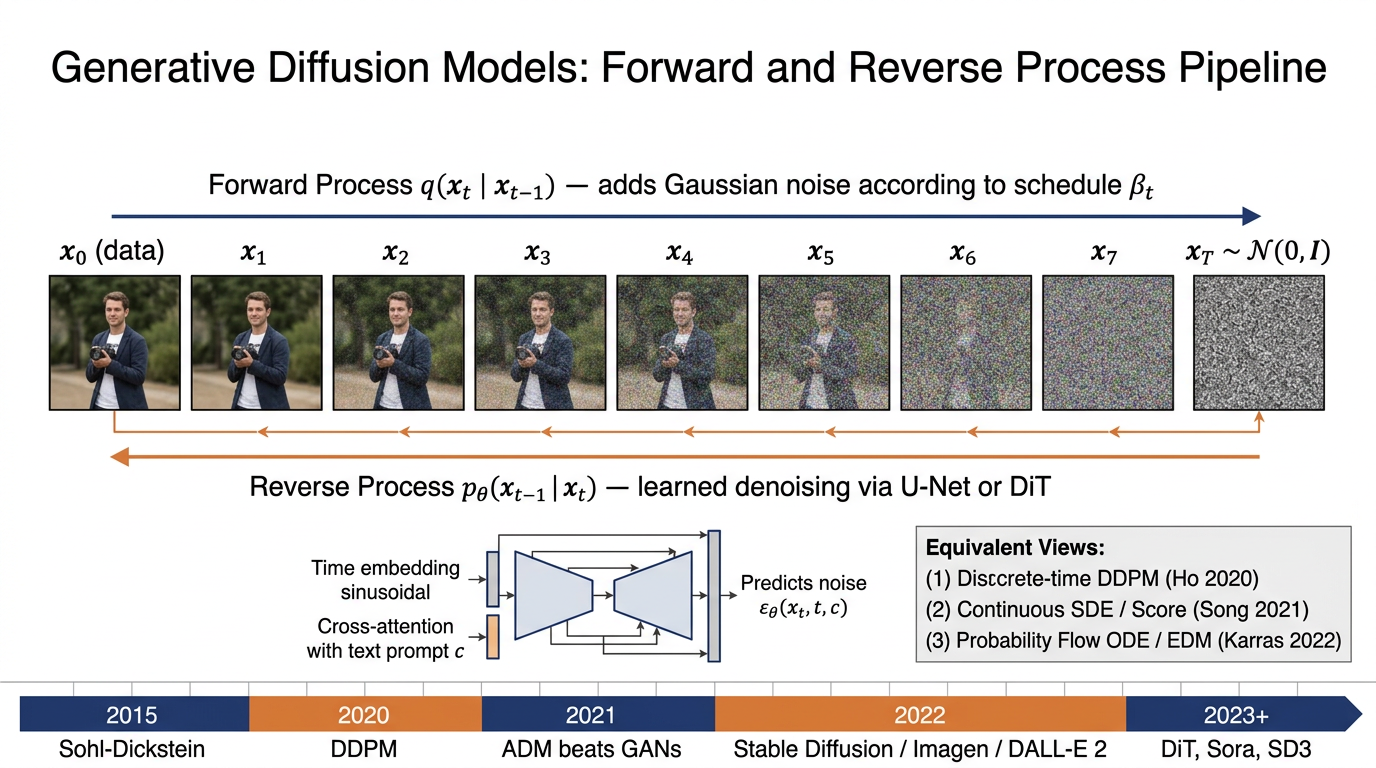
\includegraphics[keepaspectratio,alt={Forward and reverse process pipeline of generative diffusion models, with three equivalent mathematical viewpoints and a milestone timeline.}]{./figures/Generative-Diffusion-Models__fig1_pipeline.png}}
\caption{Forward and reverse process pipeline of generative diffusion models, with three equivalent mathematical viewpoints and a milestone timeline.}
\end{figure}

\section{Introduction: From Nonequilibrium Thermodynamics to Foundation Generative Models}\label{introduction-from-nonequilibrium-thermodynamics-to-foundation-generative-models}

The historical arc unfolds across five inflection points. Sohl-Dickstein, Weiss, Maheswaranathan, \& Ganguli (ICML 2015) wrote down the discrete forward chain, the variational lower bound, and the Gaussian reverse; the paper sat unused for five years. DDPM (Ho, Jain \& Abbeel, NeurIPS 2020) introduced the simplified noise-prediction loss \(L_s\)imple, the U-Net backbone with sinusoidal time embedding, and CIFAR-10 FID 3.17. The score-SDE unification (Song et al., ICLR 2021 outstanding paper) tied DDPM, NCSN, the reverse-time SDE, and the probability-flow ODE into a single framework. ADM (Dhariwal \& Nichol, NeurIPS 2021) reached ImageNet 256 FID 4.59 with classifier guidance, beating BigGAN-deep's 6.95 and triggering the GAN→diffusion rotation. The 2022--2024 deployment wave --- LDM/Stable Diffusion, GLIDE/DALL-E 2/Imagen, EDM and DPM-Solver acceleration, ControlNet, DiT-XL/2 (FID 2.27), consistency models, rectified flow, MMDiT in SD3, and Sora's 60-second 1080p video --- turned the recipe into industrial infrastructure. Section 3 documents each transition.

Empirical anchors span every modality. Image: ADM ImageNet 256 FID 4.59 (Dhariwal \& Nichol 2021), DiT-XL/2 FID 2.27 (Peebles \& Xie 2023), EDM CIFAR-10 FID 1.79 with 35 NFE (Karras et al.~2022), EDM2 ImageNet 512 FID 1.81 (Karras et al.~2024), MAR FID 1.55 (Li et al.~2024). Text-to-image: Imagen COCO-30K FID 7.27 (Saharia et al.~2022), DALL-E 2 10.39 (Ramesh et al.~2022), SD 1.5 ≈ 12.6, SD3 leads T2I-CompBench (Esser et al.~2024). Video: Imagen Video Kinetics-600 FVD ≈ 70 (Ho et al.~2022), Stable Video Diffusion 1.5B on 152M curated clips (Blattmann et al.~2023), Sora 60-second 1080p (OpenAI 2024). AudioLDM AudioSet FAD 1.97 (Liu et al.~2023). Diffusion Policy +47\% over BC across 11 Robomimic/Push-T tasks (Chi et al.~2023, RSS); RFdiffusion validated binders against HA, IL-7Rα, and SARS-CoV-2 RBD (Watson et al.~2023, \emph{Nature}).

Benchmarks: image --- CIFAR-10 (50K @ 32²), ImageNet-1K (1.28M / 1000 classes, at 64²/128²/256²/512²), CelebA-HQ, FFHQ, LSUN. Text-to-image --- COCO-30K FID, DrawBench (200 prompts), PartiPrompts (1,632 prompts × 11 categories), T2I-CompBench, GenEval, HEIM. Video --- UCF-101, Kinetics-400/600/700, WebVid-10M, HD-VILA-100M, VBench's 16-dim rubric. Audio --- LJSpeech (\textasciitilde24 h), AudioSet (\textasciitilde2M clips), MusicCaps. Training corpora include LAION-5B (5.85B image--text pairs), CC12M, Objaverse-XL (10M 3D assets), HumanML3D, the PDB (\textasciitilde220K structures), and QM9 / GEOM-DRUGS for molecules. Section 11 tabulates dominant metrics --- FID, CLIP-Score, LPIPS, FVD, FAD, KID, Vendi, HPS/ImageReward/PickScore, scRMSD --- with known biases.

Several limitations must be flagged from the start. Carlini et al.~(USENIX Security 2023) extracted \textasciitilde109 verbatim training images from Stable Diffusion 1.4 across 175M sampling attempts, and Somepalli et al.~(CVPR 2023) found \textasciitilde1.88\% of SD outputs are detectable copies of training images. Compositional binding (``a red ball and a blue cube'') fails on most systems below SD3-scale. Numeracy (``five apples'' → 3--7) is unreliable. Hand anatomy degrades into 4--6 finger artifacts without specialized data or a hand-pose ControlNet. SDXL-Turbo and LCM students close FID within \textasciitilde10\% of teachers but lose 5--10 points on prompt comprehension. Safety filters bypass via paraphrase (Rando et al.~2022). Sora exhibits identity drift after \textasciitilde30 seconds and physics violations on fluids, counts, and contact dynamics. Training SD 1.5 cost \textasciitilde150K A100-GPU-hours (\textasciitilde30 MWh, \textasciitilde10 t CO₂); SDXL \textasciitilde700K; Sora reportedly tens of millions. Copyright litigation (Getty v. Stability AI, Andersen v. Stability/Midjourney/DeviantArt, NYT v. OpenAI) is unresolved as of 2026.

Section 13 commits to three falsifiable forecasts. \emph{Forecast A:} by 31 December 2027 the leading open-weight T2I model achieves COCO-30K zero-shot FID \textless{} 7 and CLIP-Score \textgreater{} 0.32 in ≤ 4 NFE on a consumer GPU. \emph{Forecast B:} by 31 December 2027 an open or commercial video diffusion system produces coherent 5-minute 1080p video with VBench overall \textgreater{} 85. \emph{Forecast C:} by 31 December 2030 at least one FDA- or EMA-approved therapeutic biologic has a diffusion-generated lead in its discovery pipeline. We additionally expect rectified-flow/MMDiT to become the default training paradigm, consistency-style distillation to be standard, and a unified flow-matching multimodal foundation model to emerge in the 20--50B-parameter range.

Diffusion supplanted GANs because the prior paradigms left gaps. GANs (Goodfellow 2014) and their descendants (DCGAN, ProgGAN, BigGAN, StyleGAN) dominated 2014--2020 but suffered instability, mode collapse, and no tractable likelihood. VAEs (Kingma \& Welling 2014) gave likelihoods but blurry samples. Diffusion combined stable variational training with state-of-the-art quality and density estimation. The inflection point was ADM-G's ImageNet 256 FID 4.59 vs BigGAN-deep's 6.95 in 2021, and by 2024 DiT-XL/2 (FID 2.27) and SD3 had eclipsed every U-Net and GAN baseline.

The survey's scope follows from the recipe's four parts: a forward stochastic process, a learned reverse process, an objective (VLB, score matching, or flow matching), and a sampler (DDPM, DDIM, ODE, DPM-Solver). The treatment covers continuous-state Gaussian diffusion (default), discrete-state D3PM and masked diffusion for text and graphs, and manifold/equivariant diffusion for molecules and proteins.

Existing surveys cover only slices: vision-only (Croitoru 2023), T2I-only (Zhang 2023; Cao 2024), medical (Kazerouni 2022), bioinformatics (Guo 2023), audio (Zhang 2023), time series (Lin 2023), and video (Melnik 2024). Yang et al.~2023 predates DiT-scale advances, Sora, and SD3. We aim instead for a single retrieval-rich document covering mathematics, history, modalities, benchmarks, and failure modes anchored to named systems and concrete numbers.

Reading guide: §2 develops the mathematics; §3 traces 2015 → 2026 history; §4 lays out the five-axis taxonomy; §5 documents architectures; §6 covers training objectives; §7 covers sampling; §8 covers conditioning; §9 surveys modalities; §10 covers scientific applications; §11 catalogs benchmarks; §12 audits limitations; §13 forecasts; §14 concludes; §15 synthesizes critically.

For notation, x\emph{0 ∈ \(R^d\) is clean data, \(x_t\) is the noised state at time t, ε \textasciitilde{} N(0, I) is injected noise, ε}θ is the predicted noise, β\_t is the variance schedule, α\_t = 1 − β\_t, and ᾱ\_t = ∏\_s α\_s. The Stein score is ∇\_x log \(p_t\)(x). w is the CFG scale; N is the number of function evaluations (NFE).

The contributions are sixfold: (i) consolidate DDPM, score-SDE, EDM, and flow-matching into one framing; (ii) give a five-axis taxonomy through 2026; (iii) tabulate empirical anchors for every flagship system; (iv) catalog datasets and benchmarks at scale; (v) name safety, copyright, and fairness failure modes; and (vi) commit to three falsifiable 2027--2030 forecasts.

{\def\LTcaptype{none} % do not increment counter
\begin{longtable}[]{@{}
  >{\raggedright\arraybackslash}p{(\linewidth - 4\tabcolsep) * \real{0.0631}}
  >{\raggedright\arraybackslash}p{(\linewidth - 4\tabcolsep) * \real{0.2162}}
  >{\raggedright\arraybackslash}p{(\linewidth - 4\tabcolsep) * \real{0.7207}}@{}}
\toprule\noalign{}
\begin{minipage}[b]{\linewidth}\raggedright
Section
\end{minipage} & \begin{minipage}[b]{\linewidth}\raggedright
Topic
\end{minipage} & \begin{minipage}[b]{\linewidth}\raggedright
Key Anchors
\end{minipage} \\
\midrule\noalign{}
\endhead
\bottomrule\noalign{}
\endlastfoot
§2 & Mathematical foundations & DDPM ELBO; reverse-time SDE; probability-flow ODE \\
§3 & History & Sohl-Dickstein 2015 → DDPM 2020 → SDE 2021 → SD/Imagen 2022 → DiT/Sora 2023--2024 \\
§4 & Taxonomy & 5 axes, \textasciitilde12 method families \\
§5 & Architectures & U-Net (ADM), DiT, MMDiT, U-ViT \\
§6 & Training objectives & ε-, x\_0-, v-prediction; flow matching \\
§7 & Sampling & DDIM, DPM-Solver, EDM, Consistency, LCM \\
§8 & Conditioning & CFG, ControlNet, DreamBooth \\
§9 & Modality & Image, video, audio, 3D, motion, text \\
§10 & Science & RFdiffusion, GeoDiff, Diffusion Policy, DPS \\
§11 & Benchmarks & ImageNet, COCO, LAION-5B, VBench \\
§12 & Limitations & Memorization, bias, safety filters \\
§13 & Future & One-step, multimodal, theoretical unification \\
\end{longtable}
}

The survey cites the foundational primary literature --- Sohl-Dickstein 2015, Hyvärinen 2005, Vincent 2011, Anderson 1982, Song \& Ermon 2019, Ho 2020, Song 2021, Dhariwal \& Nichol 2021, Ho \& Salimans 2022, Karras 2022, Lipman 2023, Liu 2023, and Song 2023 --- alongside deployment papers (LDM, GLIDE, DALL-E 2, Imagen, SDXL, SD3, ControlNet, RFdiffusion, Sora, Diffusion Policy). The aim is keyword-searchable answers to concept, classification, historical, algorithmic, application, profiling, and prediction questions in one document.

\section{Mathematical Foundations: Forward Noising, Reverse Denoising, and Score Functions}\label{mathematical-foundations-forward-noising-reverse-denoising-and-score-functions}

This section delivers the mathematics behind the recipe of §1, in four equivalent viewpoints (discrete-time variational, score-based SDE, EDM design space, flow matching) plus a comparison table.

Three formally equivalent viewpoints derive generative diffusion. The \emph{discrete-time variational} viewpoint (Sohl-Dickstein et al.~2015; Ho, Jain, \& Abbeel, DDPM NeurIPS 2020) defines a Markov noising chain and trains the reverse via a variational lower bound. The \emph{continuous-time score-based} viewpoint (Song \& Ermon, NCSN NeurIPS 2019; Song et al., Score SDE ICLR 2021 outstanding paper) writes the same process as a stochastic differential equation and invokes Anderson's reverse-time SDE. The \emph{EDM design-space} viewpoint (Karras et al., NeurIPS 2022) treats the diffusion model as a single function F\_θ(x; σ) under preconditioning, unifying ε-, \(x_0\)-, and v-prediction. The variational diffusion viewpoint (Kingma et al., NeurIPS 2021) closes the loop by deriving a continuous-time ELBO whose value depends only on signal-to-noise ratio. All three describe a forward process that converts data to noise and a reverse process that learns the inverse; they differ in how time is indexed, what the network predicts, and how sampling is implemented. We present each, then unify them, because later sections invoke whichever framing is most convenient --- DDPM for training, score SDE for fast sampling, EDM for preconditioning, flow matching for SD3-class systems.

\subsection{Forward Markov chain and variance schedule}\label{forward-markov-chain-and-variance-schedule}

The discrete-time formulation defines a forward Markov chain q(x\emph{\{1:T\} \textbar{} \(x_0\)) = ∏}\{t=1\}\^{}T q(x\emph{t \textbar{} x}\{t-1\}) where q(x\emph{t \textbar{} x}\{t-1\}) = N(x\emph{t; √(1 − β\_t) x}\{t-1\}, β\emph{t I) is a Gaussian with a small per-step variance β\_t. Because the chain is Markovian and Gaussian, marginals admit a closed form, q(\(x_t\) \textbar{} \(x_0\)) = N(\(x_t\); √(ᾱ\_t) \(x_0\), (1 − ᾱ\_t) I), with ᾱ\_t = ∏}\{s=1\}\^{}t (1 − β\_s). This means we can sample \(x_t\) directly from \(x_0\) via the reparameterization \(x_t\) = √(ᾱ\_t) \(x_0\) + √(1 − ᾱ\_t) ε, ε \textasciitilde{} N(0, I). For T sufficiently large, ᾱ\_T ≈ 0 and \(x_T\) is approximately a standard normal.

Three variance schedules dominate the literature. Ho et al.~(DDPM, 2020) used a \emph{linear schedule}, β\emph{t = 10\^{}\{-4\} → 0.02 over T = 1000 steps, originally proposed by Sohl-Dickstein. Nichol \& Dhariwal (Improved DDPM, ICML 2021) introduced the \_cosine schedule}, ᾱ\emph{t = cos²((t/T + s)/(1 + s) · π/2), which prevents the early-step ``noising too fast'' problem and was adopted in GLIDE, DALL-E 2, Imagen, and Stable Diffusion. Karras et al.~(EDM, 2022) showed the schedule is essentially a free parameter; their \_EDM σ-schedule} parameterizes time directly by the noise standard deviation σ\_t with σ ranging in {[}0.002, 80{]} and the optimal sample distribution being a log-normal in σ. The choice of schedule materially affects sample quality: replacing linear with cosine improved ImageNet 256 FID by roughly 0.5--1.0 in the ADM ablations.

\subsection{Reverse process and the variational ELBO}\label{reverse-process-and-the-variational-elbo}

The generative model is a parameterized reverse Markov chain p\emph{θ(x}\{0:T\}) = p(x\emph{T) ∏}\{t=1\}\^{}T p\emph{θ(x}\{t-1\} \textbar{} x\emph{t), with p(\(x_T\)) = N(0, I). Each transition is parameterized as a Gaussian p}θ(x\emph{\{t-1\} \textbar{} \(x_t\)) = N(x}\{t-1\}; μ\emph{θ(\(x_t\), t), Σ}θ(x\emph{t, t)). Sohl-Dickstein et al.~(2015) showed that, when β\_t is small, this Gaussian form is sufficient to invert the forward chain. Maximizing log p}θ(x*0) is intractable, but a variational lower bound (ELBO) gives the trainable surrogate L = \(E_q\){[} −log p\emph{θ(x}0 \textbar{} \(x_1\)) + Σ\emph{\{t=2\}\^{}T D}KL(q(x\emph{\{t-1\} \textbar{} x}t, \(x_0\)) ‖ p*θ(x\_\{t-1\} \textbar{} \(x_t\))) + \(D_K\)L(q(\(x_T\) \textbar{} \(x_0\)) ‖ p(\(x_T\))) {]}.

DDPM's central simplification is to reparameterize μ\emph{θ in terms of a learned noise predictor ε}θ: μ\emph{θ(\(x_t\), t) = (1/√α\_t) {[}\(x_t\) − (β\_t / √(1 − ᾱ\_t)) ε\emph{θ(x}t, t){]}. After algebra, the ELBO terms reduce to a weighted denoising regression. Empirically, dropping the time-dependent weights and using the simple, unweighted objective \(L_s\)imple(θ) = E}\{x\emph{0, ε \textasciitilde{} N(0,I), t \textasciitilde{} U\{1,T\}\} ‖ ε − ε}θ(√(ᾱ\_t) \(x_0\) + √(1 − ᾱ\_t) ε, t) ‖² yields better samples than the exact ELBO. This is the canonical ``DDPM training loop'': sample a clean image, sample a uniform timestep, sample noise, form \(x_t\), regress ε on the U-Net's prediction. Beyond ε-prediction, alternative parameterizations include \(x_0\)-prediction (the network outputs x̂\_0), v-prediction (Salimans \& Ho 2022, used by Imagen Video and SD2 in v-mode), where \(v_t\) = √(ᾱ\_t) ε − √(1 − ᾱ\_t) \(x_0\), and direct score-prediction. Karras et al.'s EDM analyzes these reparameterizations under preconditioning and shows they are equivalent up to noise-dependent rescalings.

\subsection{Score matching, Stein scores, and reverse-time SDEs}\label{score-matching-stein-scores-and-reverse-time-sdes}

The score-based framing rephrases diffusion in terms of the (Stein) score function s*t(x) = ∇\_x log \(p_t\)(x), the gradient of the log-density of the noisy distribution at time t. Score matching (Hyvärinen 2005) proposes to learn s\emph{θ(x, t) by minimizing E}\{\(p_t\)\}{[} ‖ s\emph{θ(x, t) − ∇}x log \(p_t\)(x) ‖² {]}, a quantity that, by Hyvärinen's identity, can be computed without access to ∇\_x log \(p_t\)(x) itself. Vincent (2011) showed that \emph{denoising score matching} --- regressing s\emph{θ(x}t, t) against ∇*\{\(x_t\)\} log q(\(x_t\) \textbar{} \(x_0\)) = −(\(x_t\) − √(ᾱ\_t) \(x_0\)) / (1 − ᾱ\_t) --- yields the same optimum and is computationally cheap. Song \& Ermon (NCSN, NeurIPS 2019) trained a single noise-conditioned score network across multiple noise scales and sampled by Annealed Langevin Dynamics, achieving competitive CIFAR-10 FID before DDPM existed.

Song, Sohl-Dickstein, Kingma, Kumar, Ermon, and Poole (Score SDE, ICLR 2021 outstanding paper) made the continuous-time link explicit. They showed that the discrete forward chain is the Euler--Maruyama discretization of an SDE, dx = f(x, t) dt + g(t) dw, and that the time-reversed SDE (Anderson 1982) is dx = {[} f(x, t) − g(t)² ∇\_x log \(p_t\)(x) {]} dt + g(t) d w̄. Plugging in s\_θ(x, t) for the score gives a sampler. Two SDE families dominate: the Variance Preserving (VP) SDE, which corresponds to DDPM with β(t) interpreted as continuous; and the Variance Exploding (VE) SDE, which corresponds to NCSN. Solving the reverse SDE numerically --- Euler--Maruyama or Predictor--Corrector with Langevin steps --- yields high-quality samples but, at fine step size, requires hundreds to thousands of network evaluations.

The connection between the two viewpoints is that ε\emph{θ(\(x_t\), t) = − √(1 − ᾱ\_t) · s}θ(\(x_t\), t), so a noise-prediction network and a score-prediction network are scalar reparameterizations of each other. This is why DDPM and Score SDE are equivalent algorithms.

\subsection{Probability flow ODE and equivalent formulations}\label{probability-flow-ode-and-equivalent-formulations}

Score SDE additionally derives a \emph{probability flow ODE} whose marginals exactly match the SDE's: dx/dt = f(x, t) − ½ g(t)² ∇\emph{x log \(p_t\)(x). Because the ODE is deterministic, classical numerical solvers (Euler, Heun, Runge--Kutta) apply, and the model becomes invertible --- fundamental for likelihood evaluation, latent-space arithmetic, and editing. Karras et al.~(EDM, 2022) showed that careful preconditioning of inputs, outputs, and the loss, combined with second-order Heun integration, attains FID 1.79 on CIFAR-10 with only 35 network evaluations. Their preconditioning recipe, \(c_s\)kip(σ) x + \(c_o\)ut(σ) F}θ(\(c_i\)n(σ) x, \(c_n\)oise(σ)), unifies ε-, \(x_0\)-, and v-prediction under a single framework.

A more recent unification, \emph{flow matching} (Lipman et al.~ICLR 2023) and \emph{rectified flow} (Liu et al.~ICLR 2023), parameterizes a vector field v\emph{θ(x, t) along an interpolation path between the data and noise distributions. The conditional flow matching objective, \(L_C\)FM = E}\{t, x\emph{1, \(x_0\)\} ‖ v}θ(\(x_t\), t) − (\(x_1\) − \(x_0\)) ‖², is simpler than score matching and makes explicit the optimal-transport-style straight-line path between distributions. Rectified flow takes this further by iteratively re-flowing data along learned trajectories so they become straight lines, allowing one-step or few-step sampling. Stable Diffusion 3 (Esser et al.~ICML 2024) uses rectified flow with a Multimodal Diffusion Transformer (MMDiT) and sets new bests on T2I-CompBench and GenEval. Stochastic interpolants (Albergo, Boffi, \& Vanden-Eijnden 2023) generalize both score-based diffusion and flow matching and unify them with Schrödinger bridges. Variational diffusion models (VDM, Kingma et al.~2021) treat the schedule as learnable and provide tight likelihood bounds; CIFAR-10 VDM reaches log-likelihood 2.49 bits/dim, competitive with autoregressive models.

{\def\LTcaptype{none} % do not increment counter
\begin{longtable}[]{@{}
  >{\raggedright\arraybackslash}p{(\linewidth - 6\tabcolsep) * \real{0.1840}}
  >{\raggedright\arraybackslash}p{(\linewidth - 6\tabcolsep) * \real{0.2960}}
  >{\raggedright\arraybackslash}p{(\linewidth - 6\tabcolsep) * \real{0.3120}}
  >{\raggedright\arraybackslash}p{(\linewidth - 6\tabcolsep) * \real{0.2080}}@{}}
\toprule\noalign{}
\begin{minipage}[b]{\linewidth}\raggedright
Formulation
\end{minipage} & \begin{minipage}[b]{\linewidth}\raggedright
Forward
\end{minipage} & \begin{minipage}[b]{\linewidth}\raggedright
Reverse Mechanism
\end{minipage} & \begin{minipage}[b]{\linewidth}\raggedright
Key Reference
\end{minipage} \\
\midrule\noalign{}
\endhead
\bottomrule\noalign{}
\endlastfoot
DDPM (discrete) & Markov Gaussian chain, β\_t schedule & Ancestral sampling, ε-prediction U-Net & Ho et al.~NeurIPS 2020 \\
NCSN & Multi-scale Gaussian noise & Annealed Langevin Dynamics & Song \& Ermon NeurIPS 2019 \\
Score SDE (VP/VE) & Continuous Itô SDE & Reverse-time SDE / probability flow ODE & Song et al.~ICLR 2021 \\
EDM & σ-parameterized noising & Heun integrator + preconditioning & Karras et al.~NeurIPS 2022 \\
Variational Diffusion & Continuous SNR(t) & Likelihood-tight ELBO & Kingma et al.~NeurIPS 2021 \\
Flow Matching & Linear interp x\_t = (1−t) x\_0 + t x\_1 & Vector-field ODE & Lipman et al.~ICLR 2023 \\
Rectified Flow & Straight-line interpolant & Iterative rectification, few-step & Liu et al.~ICLR 2023 \\
Stochastic Interpolants & General interpolant & SDE+ODE unified & Albergo et al.~2023 \\
\end{longtable}
}

Each view matters for a different reason. DDPM underpins the training loop, SDE/ODE enables fast sampling, EDM preconditioning stabilizes training across noise scales, and flow matching powers SD3, Lumina, and 2024--2026 frontier systems. The unification explains why FID on ImageNet 256 fell from 4.59 (ADM, 2021) to 2.27 (DiT-XL/2, 2023) to under 2.0 (EDM2, SiT-XL, MAR) within four years.

The framework connects cleanly to other generative paradigms. A diffusion model is an infinite-depth hierarchical VAE (Kingma 2021), and the probability-flow ODE makes it a continuous normalizing flow. Adversarial distillation (StyleGAN-T, SDXL-Turbo) plugs a GAN discriminator on top, while energy-based models and diffusion converge in the small-noise limit. Nearly every prior generative paradigm is recoverable as a special case.

Computational complexity is simple. Training cost scales as epochs × batch × model FLOPs, and inference cost is \(N_s\)teps × per-step forward. SD 1.5 at 50 DDIM steps on one A100 takes \textasciitilde3.5s, and LDM cuts pixel cost by f² ≈ 64 via the autoencoder bottleneck.

Section 3 traces how the field arrived at this consensus, from Sohl-Dickstein 2015 through the 2024 deployment wave.

\section{Historical Trajectory: From Sohl-Dickstein 2015 to Sora 2024}\label{historical-trajectory-from-sohl-dickstein-2015-to-sora-2024}

\begin{figure}
\centering
\pandocbounded{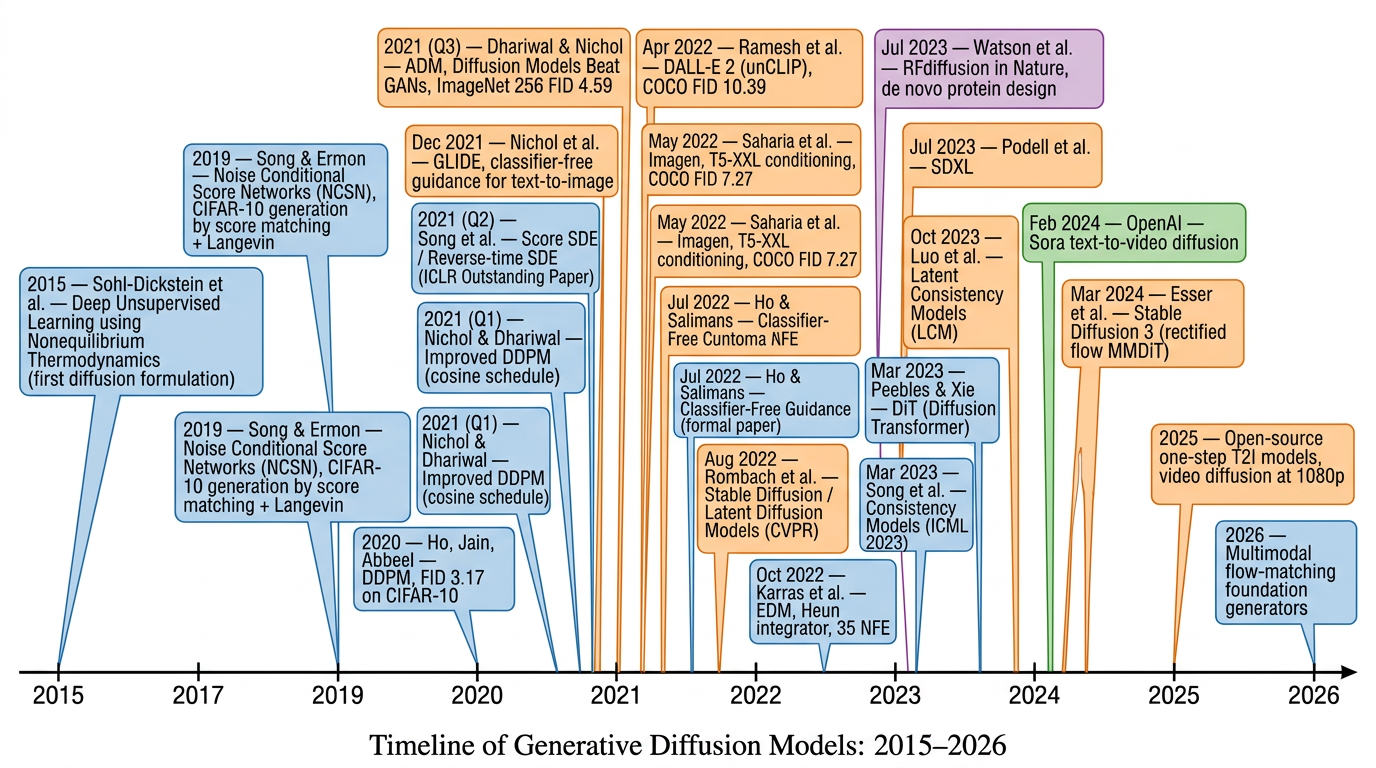
\includegraphics[keepaspectratio,alt={Timeline of generative diffusion milestones from Sohl-Dickstein (2015) to SD3, Sora, and beyond.}]{./figures/Generative-Diffusion-Models__fig5_timeline.png}}
\caption{Timeline of generative diffusion milestones from Sohl-Dickstein (2015) to SD3, Sora, and beyond.}
\end{figure}

This section traces how the four mathematical viewpoints arrived in practice between 2015 and 2026, in four phases plus a milestone table. Early origins begin with Sohl-Dickstein et al.~(2015, original ELBO + Markov chain) and NCSN (2019, multi-scale score matching). The DDPM/SDE breakthrough arrived through DDPM (2020, simplified ε-loss with U-Net), DDIM (2021, deterministic non-Markovian sampler), Improved DDPM (2021, cosine schedule + learned variance), Score SDE (2021, reverse-time SDE unification), and ADM (2021, ImageNet 256 FID 4.59 with classifier guidance). The text-to-image scaling era opened with GLIDE (2021, T2I + CFG) and continued with DALL-E 2 (2022, unCLIP), Imagen (2022, T5-XXL cascade), LDM / Stable Diffusion (2022, factor-8 latent), EDM (2022, Heun + preconditioning), and DPM-Solver (2022, closed-form ODE). Consolidation followed with ControlNet (2023, structural conditioning), DiT (2023, ImageNet 256 FID 2.27), Consistency Models (2023, 1--4-step generation), SDXL (2023, 2.6B U-Net), RFdiffusion (2023, de novo protein binders in \emph{Nature}), and LCM (2023, 4-step SDXL distillation). Sora (2024) delivered 60-second 1080p video, and SD3 / MMDiT (2024) introduced rectified flow at 8B parameters.

The history of generative diffusion is unusually compressed. A 2015 theoretical proposal sat nearly dormant for five years, then in 36 months --- June 2020 (DDPM) through February 2024 (Sora) --- became the dominant generative paradigm across every modality this survey examines. We organize the trajectory into four phases: early origins (1995--2019), the DDPM/SDE breakthrough (2020--2021), the text-to-image scaling era (2021--2022), and the DiT/rectified-flow consolidation (2023--2026). For each phase we identify the bottleneck --- sample quality, training stability, conditioning, inference cost, scaling --- whose resolution unlocked the next deployment frontier. The named anchors used as section signposts are: Sohl-Dickstein 2015 (ELBO), Song \& Ermon 2019 (NCSN, CIFAR-10 FID 25.3), Ho et al.~2020 (DDPM, CIFAR-10 FID 3.17), Song et al.~2021 (score SDE), Dhariwal \& Nichol 2021 (ADM, ImageNet 256 FID 4.59), Rombach et al.~2022 (LDM/Stable Diffusion), Karras et al.~2022 (EDM, FID 1.79), Peebles \& Xie 2023 (DiT, FID 2.27), Song et al.~2023 (consistency models, 1--4 NFE), Esser et al.~2024 (SD3/MMDiT), and OpenAI 2024 (Sora, 60-second 1080p video).

\subsection{Early origins and score matching (1995--2019)}\label{early-origins-and-score-matching-19952019}

Score-based reasoning predates diffusion. Hyvärinen (2005) introduced \emph{score matching} as a way to fit unnormalized statistical models without computing the partition function. Vincent (2011) connected denoising autoencoders to score estimation, showing that learning to denoise is implicitly learning ∇\_x log \(p_t\)(x). The reverse-time stochastic differential equation, central to modern continuous-time diffusion, was derived by Anderson (1982) decades earlier in stochastic control. None of this was used for generative modeling at scale.

The pivotal early generative-modeling paper is Sohl-Dickstein, Weiss, Maheswaranathan, and Ganguli, ``Deep Unsupervised Learning using Nonequilibrium Thermodynamics'' (ICML 2015). They proposed the discrete forward Markov chain, the variational lower bound, and the parameterized reverse Gaussian --- essentially every ingredient of modern DDPM. However, the experiments used small models on simple datasets (CIFAR-10 grayscale, MNIST, dead-leaves) and the paper was overshadowed by the rapid rise of GANs (Goodfellow et al.~2014, Radford et al.~DCGAN 2016, Karras et al.~ProgGAN 2018, BigGAN 2018, StyleGAN 2019). The 2015 paper accumulated under 200 citations in its first three years.

The next decisive step was Yang Song \& Stefano Ermon's \emph{Generative Modeling by Estimating Gradients of the Data Distribution} (NeurIPS 2019), introducing Noise Conditional Score Networks (NCSN). They observed that data lies on a low-dimensional manifold, so estimating ∇\_x log \(p_d\)ata(x) by score matching is unstable; injecting noise at multiple scales and training a single network to predict the score at each scale solves this. Sampling via Annealed Langevin Dynamics across decreasing noise scales generated CIFAR-10 images with FID ≈ 25.32 --- better than NICE, Real NVP, and competitive with early GAN baselines. This paper put score matching back on the map for high-dimensional generative modeling.

\subsection{The DDPM/SDE breakthrough (2020--2021)}\label{the-ddpmsde-breakthrough-20202021}

The decisive empirical result came in June 2020 when Jonathan Ho, Ajay Jain, and Pieter Abbeel posted \emph{Denoising Diffusion Probabilistic Models} (DDPM, NeurIPS 2020). Three innovations turned Sohl-Dickstein's framework into a top-tier generative model. First, a U-Net (Ronneberger et al.~2015) backbone with sinusoidal time embedding, group normalization, attention at the lowest resolution, and skip connections --- the architecture borrowed from PixelCNN++ and ProgGAN. Second, the simplified objective \(L_s\)imple regressing predicted noise on true noise, which empirically outperforms the exact ELBO on sample quality. Third, the algebraic equivalence between ε-prediction and the score, made explicit. Ho et al.~reported FID 3.17 on CIFAR-10 (10× better than the 2015 paper) and competitive 256×256 LSUN samples, with T = 1000 timesteps and a linear β schedule.

Within months, Jiaming Song, Chenlin Meng, and Stefano Ermon proposed \emph{Denoising Diffusion Implicit Models} (DDIM, ICLR 2021), exploiting that the marginals q(x\emph{t \textbar{} \(x_0\)) are the same regardless of the underlying chain's Markov structure, so a deterministic non-Markovian sampler with 50 steps could match the quality of 1000-step DDPM. DDIM is the basis of essentially every fast diffusion sampler that followed. Concurrently, Nichol \& Dhariwal's }Improved DDPM* (ICML 2021) added the cosine schedule and learned variance Σ*θ, lowering CIFAR-10 NLL.

The unifying framework arrived in November 2020 with \emph{Score-Based Generative Modeling through Stochastic Differential Equations} by Song, Sohl-Dickstein, Kingma, Kumar, Ermon, and Poole (ICLR 2021 Outstanding Paper). They cast both DDPM and NCSN as discretizations of an Itô SDE, derived the reverse-time SDE, introduced the probability-flow ODE, and showed that VP and VE families both arise naturally. This paper provided the toolbox for the dozens of fast samplers and likelihood evaluators that followed.

May 2021 brought the empirical sledgehammer. Prafulla Dhariwal and Alex Nichol's \emph{Diffusion Models Beat GANs on Image Synthesis} (NeurIPS 2021) introduced the \emph{Ablated Diffusion Model} (ADM): a much larger U-Net (\textasciitilde553M parameters), classifier guidance leveraging gradients of an auxiliary noise-aware ImageNet classifier, learned variance heads, and improvements such as adaptive group normalization. ADM-G achieved ImageNet 128×128 FID 2.97, ImageNet 256×256 FID 4.59, and ImageNet 512×512 FID 7.72, surpassing BigGAN-deep on every resolution. This was the moment the generative-modeling community rotated toward diffusion.

\subsection{The text-to-image explosion (2021--2022)}\label{the-text-to-image-explosion-20212022}

December 2021 brought GLIDE (Nichol et al.), the first text-to-image diffusion system at scale. GLIDE used a 3.5B U-Net with text-conditioned cross-attention and \emph{classifier-free guidance} (CFG), an idea Ho \& Salimans later wrote up formally in July 2022. CFG removes the need for a separate noisy-image classifier by training the conditional and unconditional models jointly (with prompt drop-out at probability \textasciitilde0.1) and combining their predictions at inference. GLIDE reported COCO-30K zero-shot FID of 12.24 with 100 sampling steps, competitive with auto-regressive DALL-E despite using one-tenth the parameters.

April 2022 was DALL-E 2 / unCLIP from Aditya Ramesh and colleagues at OpenAI: a CLIP-image-prior diffusion stage feeding a CLIP-conditioned image diffusion decoder, with a cascade of upsamplers from 64×64 to 1024×1024. DALL-E 2's COCO-30K FID was 10.39. May 2022 brought Google's Imagen (Saharia, Chan, Saxena et al., NeurIPS 2022) using a frozen 4.6B-parameter T5-XXL text encoder and three-stage diffusion cascade (64→256→1024); Imagen achieved FID 7.27 on COCO and dramatic improvements in prompt comprehension. eDiff-I (NVIDIA), Parti (Google, an AR baseline), and CogView-2 followed.

The democratizing event came in August 2022 with Robin Rombach, Andreas Blattmann, Dominik Lorenz, Patrick Esser, and Björn Ommer's \emph{High-Resolution Image Synthesis with Latent Diffusion Models} (CVPR 2022). LDM ran the diffusion U-Net inside the bottleneck of a pre-trained VQ-GAN/KL autoencoder (downsampling factor f = 4 or 8), reducing pixel cost by 16--64×. The Stability AI / RunwayML release of \emph{Stable Diffusion 1.4} in August 2022, followed by Stable Diffusion 1.5 (October 2022) and 2.1 (December 2022), put a 860M-parameter, 512×512 text-to-image model into open-source hands. Stable Diffusion was trained on the LAION-aesthetics-v2-5+ subset of LAION-5B (Schuhmann et al.~2022), which contains 5.85 billion image--text pairs.

October 2022 also brought EDM (Karras et al., NeurIPS 2022), which set new state-of-the-art FID 1.79 on CIFAR-10 with 35 NFE and clarified how to design the noise schedule and preconditioning. Lu et al.'s DPM-Solver (NeurIPS 2022) provided a high-order ODE solver that hit comparable FID with ≤10 NFE, enabling sub-second SD inference.

\subsection{The DiT, video, and rectified-flow era (2023--2026)}\label{the-dit-video-and-rectified-flow-era-20232026}

February 2023 introduced ControlNet (Lvmin Zhang \& Maneesh Agrawala, ICCV 2023), a hypernetwork that adds structural conditioning (Canny edges, depth, pose, segmentation) to a frozen Stable Diffusion U-Net via copy-and-zero-init residual connections. T2I-Adapter (Mou et al.~2024 AAAI) and IP-Adapter generalized this to text-feature, image-prompt, and style adapters.

March 2023 was a watershed. Peebles \& Xie's \emph{Scalable Diffusion Models with Transformers} (DiT, ICCV 2023) replaced the U-Net with a Vision-Transformer-style backbone using adaLN-Zero conditioning. DiT-XL/2 reached FID 2.27 on ImageNet 256×256, beating ADM-G. Critically, DiT showed clean scaling laws --- Gflops vs.~FID --- establishing the path to ever-larger diffusion models. The same month, Yang Song, Prafulla Dhariwal, Mark Chen, and Ilya Sutskever introduced \emph{Consistency Models} (ICML 2023), training a single function f\emph{θ(\(x_t\), t) → \(x_0\) to be self-consistent across timesteps; consistency models generated competitive samples in 1--4 steps. The pace continued with \_Latent Consistency Models} (Luo et al.~2023), which distilled Stable Diffusion into a 2--4-step generator (\textasciitilde400ms per 1024² SDXL image), and SDXL-Turbo / ADD (Sauer et al.~2023), an adversarial distillation producing 1-step images.

July 2023 was SDXL (Podell et al.): a 2.6B-parameter U-Net trained on a curated subset of LAION, with two text encoders (OpenCLIP-ViT/G and CLIP-ViT/L) and refinement at 1024×1024. SDXL became the de-facto open-source standard. The same week, Watson, Juergens, Bennett et al.'s \emph{RFdiffusion} appeared in Nature, demonstrating de novo protein backbone design via diffusion conditioned on RoseTTAFold. Ingraham et al.'s \emph{Chroma} (Nature 2023) provided a programmable generative model for proteins.

December 2023 saw Stable Video Diffusion (Blattmann et al.), a 1.5B-parameter latent video diffusion model trained on a curated 152M-clip dataset, generating 2--4 second clips at 1024×576. February 2024, OpenAI revealed \emph{Sora}, a DiT-style spatiotemporal-patch diffusion model generating up to 60-second 1080p videos, dramatically extending coherent video duration. Stable Diffusion 3 / MMDiT (Esser et al.~ICML 2024) shipped in early 2024, switching from ε-prediction to rectified flow and introducing the Multimodal Diffusion Transformer that processes text and image tokens with shared attention --- the basis for follow-up systems including Pixart-Σ, Flux, Lumina-Next, and Hunyuan-DiT.

By 2026, the field has consolidated around three threads: (i) flow-matching / rectified-flow training as the default, supplanting strict DDPM noise prediction; (ii) Diffusion Transformers as the universal backbone for image, video, and 3D; and (iii) one-step or few-step inference via consistency-based or adversarial distillation, narrowing the quality--latency gap.

{\def\LTcaptype{none} % do not increment counter
\begin{longtable}[]{@{}
  >{\raggedright\arraybackslash}p{(\linewidth - 4\tabcolsep) * \real{0.0889}}
  >{\raggedright\arraybackslash}p{(\linewidth - 4\tabcolsep) * \real{0.4889}}
  >{\raggedright\arraybackslash}p{(\linewidth - 4\tabcolsep) * \real{0.4222}}@{}}
\toprule\noalign{}
\begin{minipage}[b]{\linewidth}\raggedright
Year
\end{minipage} & \begin{minipage}[b]{\linewidth}\raggedright
Milestone
\end{minipage} & \begin{minipage}[b]{\linewidth}\raggedright
Anchor Fact
\end{minipage} \\
\midrule\noalign{}
\endhead
\bottomrule\noalign{}
\endlastfoot
2015 & Sohl-Dickstein et al., diffusion formulation & First ELBO + Markov chain \\
2019 & Song \& Ermon NCSN & CIFAR-10 FID ≈ 25.3 via score matching \\
Jun 2020 & Ho et al.~DDPM & CIFAR-10 FID 3.17 \\
Oct 2020 & DDIM (Song, Meng, Ermon) & 50-step deterministic sampling \\
Feb 2021 & Improved DDPM & Cosine schedule \\
May 2021 & Score SDE (Song et al.) & Reverse-time SDE unification \\
May 2021 & ADM (Dhariwal \& Nichol) & ImageNet 256 FID 4.59, beats BigGAN \\
Dec 2021 & GLIDE & T2I + CFG, COCO FID 12.24 \\
Apr 2022 & DALL-E 2 / unCLIP & COCO FID 10.39 \\
May 2022 & Imagen & T5-XXL, COCO FID 7.27 \\
Aug 2022 & Stable Diffusion / LDM & 860M U-Net, factor-8 latent \\
Oct 2022 & EDM (Karras et al.) & CIFAR-10 FID 1.79, 35 NFE \\
Feb 2023 & ControlNet & Structural T2I conditioning \\
Mar 2023 & DiT (Peebles \& Xie) & ImageNet 256 FID 2.27 \\
Mar 2023 & Consistency Models & 1--4 step generation \\
Jul 2023 & SDXL & 2.6B U-Net \\
Jul 2023 & RFdiffusion (Nature) & De novo protein design \\
Oct 2023 & LCM / LCM-LoRA & 2--4 step SDXL distillation \\
Feb 2024 & Sora (OpenAI) & 60s 1080p video diffusion \\
Mar 2024 & SD3 / MMDiT (Esser et al.) & Rectified flow, 8B parameters \\
2025 & Flux, Pixart-Σ, Lumina-Next & Open MMDiT-style frontier \\
2026 & Multimodal flow-matching foundations & Any-to-any generation \\
\end{longtable}
}

Each transition resolved a concrete bottleneck. DDPM (2020) replaced the brittle exact ELBO with \(L_s\)imple, ADM (2021) used classifier guidance plus larger U-Nets to clear the GAN bar on ImageNet, LDM (2022) cut pixel cost via the autoencoder bottleneck, DiT (2023) inherited transformer scaling laws, and SD3 / MMDiT (2024) showed rectified flow trains more stably at multi-billion-parameter scale and admits cleaner one-step distillation. The pattern is that a theoretical idea matures when paired with a curated dataset (ImageNet → LAION-5B → curated video corpora) and one or two engineering tricks (cosine schedule, CFG, latent autoencoder, rectified flow). Section 4 turns this historical succession into a five-axis taxonomy.

\section{Taxonomy of Generative Diffusion Methods}\label{taxonomy-of-generative-diffusion-methods}

\begin{figure}
\centering
\pandocbounded{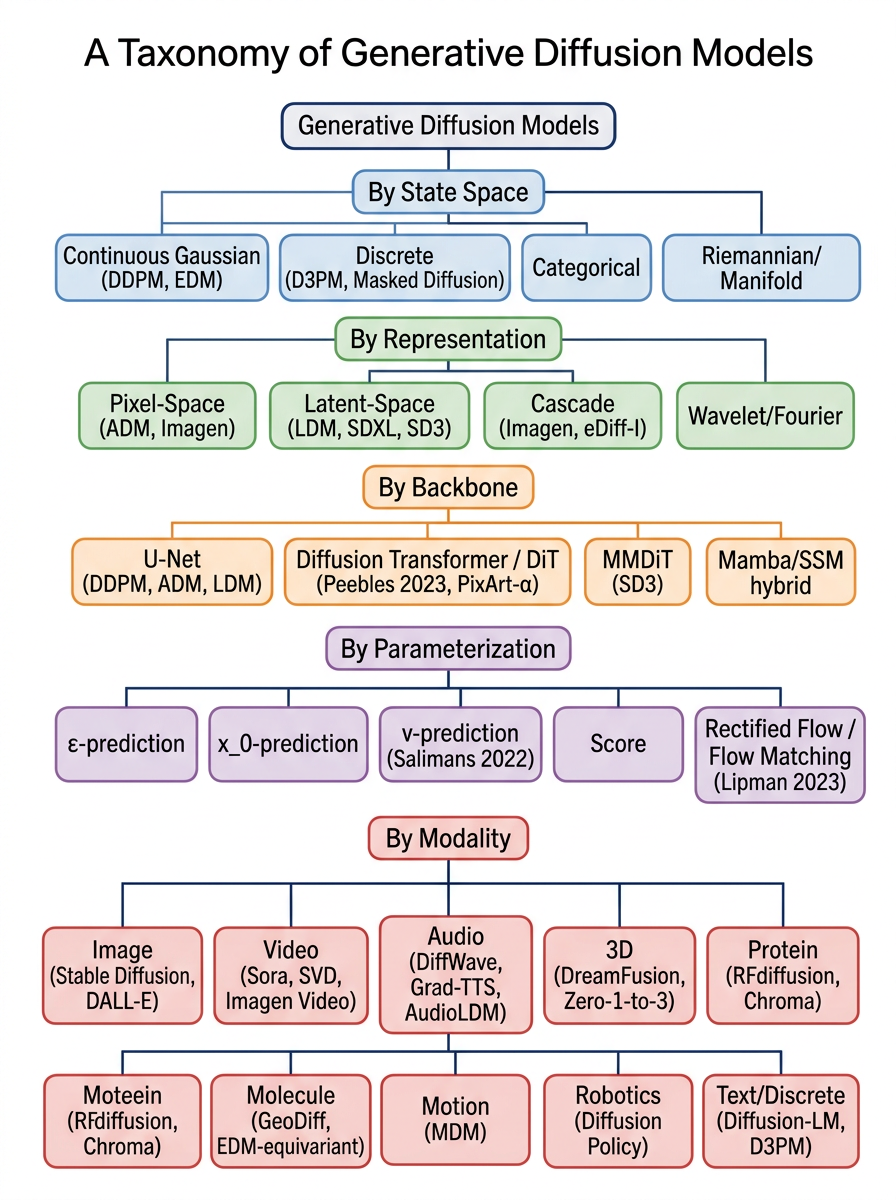
\includegraphics[keepaspectratio,alt={Vertical taxonomy tree organizing diffusion models along five axes: state space, representation, backbone, parameterization, modality.}]{./figures/Generative-Diffusion-Models__fig2_taxonomy.png}}
\caption{Vertical taxonomy tree organizing diffusion models along five axes: state space, representation, backbone, parameterization, modality.}
\end{figure}

This section converts §3's chronology into a coordinate system, delivering a five-axis taxonomy (state space, representation, backbone, parameterization, modality) that locates every major method family.

Diffusion models vary along many independent axes --- what to noise, where to noise, what backbone, what loss, what modality --- so a flat list misses the structure. We propose five axes that account for every published variant through 2026 and name the canonical method for each cell. The axes are mutually consistent: a concrete system is a 5-tuple (state space, representation, backbone, parameterization, modality), and most empirical advances combine an innovation on one axis with stable choices on the others. As a sanity check, Stable Diffusion 1.5 = (continuous, latent f=8, U-Net, ε, image); SD3 = (continuous, latent 16-channel, MMDiT, rectified flow, image); RFdiffusion = (manifold SE(3), residue graph, RoseTTAFold, score, protein); Diffusion Policy = (continuous, action trajectory, 1D U-Net, ε, robot action); DreamFusion = (continuous, NeRF-as-latent, frozen 2D prior with SDS, ε, 3D). Sections 5--8 expand on architecture, training, sampling, and conditioning; §9--§10 walk through modality-specific deployments; §11 anchors each cell to the benchmark on which it is evaluated.

\subsection{By state space: continuous, discrete, and manifold diffusion}\label{by-state-space-continuous-discrete-and-manifold-diffusion}

\textbf{Continuous Gaussian diffusion} is the default. The forward process adds Gaussian noise to a real-valued tensor x ∈ \(R^d\); the reverse process is parameterized as a Gaussian transition. This is the regime of DDPM (Ho et al.~2020), Score SDE (Song et al.~2021), ADM (Dhariwal \& Nichol 2021), Stable Diffusion (Rombach et al.~2022), DiT (Peebles \& Xie 2023), and almost all image, video, and audio systems. Within continuous diffusion, the two main subtypes are \emph{Variance Preserving} (VP, used by DDPM, ADM, Stable Diffusion) and \emph{Variance Exploding} (VE, used by NCSN, EDM); they correspond to different choices of forward drift and diffusion coefficients and yield slightly different sample-quality / step-count tradeoffs.

\textbf{Discrete diffusion} operates over discrete state spaces --- categorical tokens for text, atom types for molecules, edges for graphs. Austin et al.'s \emph{D3PM} (NeurIPS 2021) introduced absorbing-state, uniform, and Gaussian-discrete transitions. Hoogeboom et al.~proposed \emph{Multinomial Diffusion} for categorical data. \emph{Masked diffusion} (recently popular in NLP) makes the absorbing-state special case explicit, mirroring BERT-style infilling. Diffusion-LM (Li et al.~2022) instead embeds tokens into continuous latents, then applies continuous diffusion. Discrete diffusion has been adopted in DiscoBax for molecular property prediction, MolDiff for molecules, and DiffSeq for protein sequences (EvoDiff).

\textbf{Manifold and equivariant diffusion} runs the forward and reverse processes on Riemannian manifolds or imposes group symmetries. Hoogeboom, Satorras, Vignac, and Welling's \emph{Equivariant Diffusion Model} (EDM, ICML 2022) builds a SE(3)-equivariant E(n) GNN to generate 3D molecule conformations that are invariant to rotation/translation. RFdiffusion uses SE(3)-equivariant message passing on protein backbones. \emph{Riemannian score-based generative modeling} (De Bortoli et al.~2022) extends diffusion to spheres, tori, and other manifolds for directional or rotational data. This axis matters in scientific applications where the data has known geometric structure.

\subsection{By representation: pixel, latent, cascade, wavelet, Fourier}\label{by-representation-pixel-latent-cascade-wavelet-fourier}

\textbf{Pixel-space diffusion} runs the U-Net or DiT directly on the data tensor. ADM, Imagen base, GLIDE, EDM, and CIFAR-10 / ImageNet 256 baselines all operate in pixel space. The advantage is straightforward likelihood; the disadvantage is high inference cost at high resolution.

\textbf{Latent diffusion} encodes data with a frozen autoencoder before diffusion. Rombach et al.'s LDM (CVPR 2022) uses a VQ-GAN or KL-regularized autoencoder with downsampling factor f ∈ \{4, 8\}; SDXL uses f = 8 with a 4-channel latent. SD3's MMDiT operates on a 16-channel KL-VAE latent. AudioLDM uses a mel-spectrogram autoencoder. The latent representation reduces compute by f² while sacrificing some pixel-level detail.

\textbf{Cascade diffusion} stacks a base model (low resolution, e.g., 64×64) with one or more super-resolution diffusion stages (256→1024). Imagen, eDiff-I, and DALL-E 2 use 2--3 stage cascades. Each stage can use a smaller U-Net at its own resolution; the cascade structure permits prompt comprehension at low resolution and detail at high resolution.

\textbf{Wavelet/Fourier diffusion} trains the model on a frequency-domain decomposition of the data. Wavelet Diffusion Models (WDM) and Fourier-domain audio diffusion compute the diffusion process in a frequency basis, which can speed up training on data with strong spectral structure (audio, structured images).

\subsection{By backbone: U-Net, DiT, U-ViT, hybrid SSM}\label{by-backbone-u-net-dit-u-vit-hybrid-ssm}

\textbf{U-Net} is the original DDPM and ADM backbone. Stable Diffusion 1.5 uses an 860M-parameter U-Net with cross-attention at multiple resolutions; SDXL uses a 2.6B-parameter U-Net with two text encoders. U-Nets are convolutional, multi-resolution, and inductively biased for spatial coherence --- a strong default for image generation up to 1024×1024.

\textbf{Diffusion Transformer (DiT)} was introduced by Peebles \& Xie (ICCV 2023). Patches of the latent are tokenized; a stack of transformer blocks with adaLN-Zero conditioning processes them; FID scaling tracks transformer FLOPs. DiT-XL/2 has 675M parameters and reaches FID 2.27 on ImageNet 256. PixArt-α (Chen et al.~ICLR 2024) demonstrated that DiT can be trained for text-to-image with \textasciitilde10× lower compute than SDXL. Sora's backbone is a DiT-style spatiotemporal patch transformer.

U-ViT and hybrid backbones extend the basic family. U-ViT (Bao et al.~2022) uses a hybrid U-shape with transformer blocks. \emph{Multimodal DiT} (MMDiT, Esser et al.~2024) processes text and image tokens jointly with shared attention. \emph{DiffiT} (Hatamizadeh et al.~ECCV 2024) uses a hybrid attention mechanism. \emph{Diffusion Mamba} (Mo \& Tian 2024) uses bidirectional state-space models for efficient long-context video.

\textbf{Conditioning modules} that ride on top of any backbone include cross-attention layers (used by all T2I systems), ControlNet (Zhang \& Agrawala 2023, hypernetwork copies of encoder blocks), T2I-Adapter (lightweight adapter modules), IP-Adapter (image-prompt adapter), DreamBooth (full fine-tuning with class-prior preservation), Textual Inversion (learning a new token embedding), and LoRA (low-rank weight adapters). These are orthogonal to the backbone choice.

\subsection{\texorpdfstring{By parameterization: ε, \(x_0\), v, score, flow}{By parameterization: ε, x\_0, v, score, flow}}\label{by-parameterization-ux3b5-x_0-v-score-flow}

\textbf{ε-prediction} is the DDPM default: ε\_θ(\(x_t\), t) regresses the injected Gaussian noise. Used by Stable Diffusion 1.5, ADM, GLIDE, Imagen.

\textbf{\(x_0\)-prediction} trains the network to predict the clean datum directly. Used in some segmentation diffusion models and as a target for distillation.

\textbf{v-prediction} (Salimans \& Ho, 2022 progressive distillation paper) defines \(v_t\) = √ᾱ\_t · ε − √(1−ᾱ\_t) · \(x_0\) as a balanced target that interpolates between ε and \(x_0\). Used by Stable Diffusion 2.1 (in v-mode) and Imagen Video.

\textbf{Score-prediction} trains s\_θ to estimate ∇\_x log \(p_t\)(x). Algebraically equivalent to ε-prediction up to a noise-dependent rescaling, but used explicitly in some scientific applications.

\textbf{Flow / vector-field prediction} (Lipman 2023, Liu 2023) trains a velocity field v\_θ(x, t) along a straight-line interpolant between data and noise. Stable Diffusion 3, Lumina, and Pixart-Σ all use this parameterization. Rectified flow's iterative re-flow procedure further straightens trajectories for one-step generation.

{\def\LTcaptype{none} % do not increment counter
\begin{longtable}[]{@{}
  >{\raggedright\arraybackslash}p{(\linewidth - 6\tabcolsep) * \real{0.0833}}
  >{\raggedright\arraybackslash}p{(\linewidth - 6\tabcolsep) * \real{0.3750}}
  >{\raggedright\arraybackslash}p{(\linewidth - 6\tabcolsep) * \real{0.4167}}
  >{\raggedright\arraybackslash}p{(\linewidth - 6\tabcolsep) * \real{0.1250}}@{}}
\toprule\noalign{}
\begin{minipage}[b]{\linewidth}\raggedright
Axis
\end{minipage} & \begin{minipage}[b]{\linewidth}\raggedright
Categories
\end{minipage} & \begin{minipage}[b]{\linewidth}\raggedright
Representative Systems
\end{minipage} & \begin{minipage}[b]{\linewidth}\raggedright
Year
\end{minipage} \\
\midrule\noalign{}
\endhead
\bottomrule\noalign{}
\endlastfoot
State space & Continuous Gaussian / Discrete (D3PM) / Manifold (EDM) & Stable Diffusion / Diffusion-LM / RFdiffusion & 2020/2021/2023 \\
Representation & Pixel / Latent / Cascade / Wavelet & ADM / LDM / Imagen / WDM & 2021/2022/2022/2023 \\
Backbone & U-Net / DiT / U-ViT / Mamba & SD 1.5 / DiT-XL / Pixart-α / DiM & 2020/2023/2023/2024 \\
Parameterization & ε / x\_0 / v / score / flow & DDPM / Imagen-Video / SD3 & 2020/2022/2024 \\
Conditioning & Class / Text / Image / Structure / Sound & ADM / SDXL / DreamBooth / ControlNet / AudioLDM & 2021/2023/2023/2023/2023 \\
Modality & Image / Video / Audio / 3D / Protein / Motion / Text / Robotics & SD / Sora / DiffWave / DreamFusion / RFdiffusion / MDM / D3PM / Diffusion Policy & 2020--2024 \\
Sampling & DDPM / DDIM / DPM-Solver / EDM Heun / Consistency / LCM / Rectified Flow & Various & 2020--2024 \\
\end{longtable}
}

\subsection{Cross-axis combinations}\label{cross-axis-combinations}

Most deployed systems combine choices across axes. Stable Diffusion 1.5 = (continuous, latent f=8, U-Net, ε-prediction, text-conditional, image). SDXL = (continuous, latent f=8, larger U-Net, ε-prediction, text-conditional, image). SD3 = (continuous, latent f=8 with 16-channel VAE, MMDiT, rectified-flow, text-conditional, image). Imagen Video = (continuous, pixel cascade, U-Net 3D, v-prediction, text-conditional, video). RFdiffusion = (continuous on SE(3), pixel-equivalent backbone graph, RoseTTAFold encoder, score-prediction, structure-conditional, protein). Diffusion Policy = (continuous, observation-conditioned trajectory, 1D U-Net, ε-prediction, vision-conditional, action). The taxonomy is therefore not a strict hierarchy but a coordinate system.

\subsection{Why this taxonomy and not others}\label{why-this-taxonomy-and-not-others}

Earlier surveys (Yang et al.~2023; Croitoru et al.~2023; Cao et al.~2024) proposed two- or three-axis taxonomies focused on application area or sampling scheme. Such taxonomies miss the cross-cutting nature of recent advances. Our five-axis taxonomy separates representation, backbone, and parameterization, so questions like ``what would a manifold-DiT for proteins look like?'' become well-posed and underexplored combinations (manifold + latent + DiT) become visible.

\subsection{Method-family comparison table}\label{method-family-comparison-table}

{\def\LTcaptype{none} % do not increment counter
\begin{longtable}[]{@{}
  >{\raggedright\arraybackslash}p{(\linewidth - 10\tabcolsep) * \real{0.1583}}
  >{\raggedright\arraybackslash}p{(\linewidth - 10\tabcolsep) * \real{0.1583}}
  >{\raggedright\arraybackslash}p{(\linewidth - 10\tabcolsep) * \real{0.2158}}
  >{\raggedright\arraybackslash}p{(\linewidth - 10\tabcolsep) * \real{0.1655}}
  >{\raggedright\arraybackslash}p{(\linewidth - 10\tabcolsep) * \real{0.1151}}
  >{\raggedright\arraybackslash}p{(\linewidth - 10\tabcolsep) * \real{0.1871}}@{}}
\toprule\noalign{}
\begin{minipage}[b]{\linewidth}\raggedright
Family
\end{minipage} & \begin{minipage}[b]{\linewidth}\raggedright
Canonical paper
\end{minipage} & \begin{minipage}[b]{\linewidth}\raggedright
Backbone
\end{minipage} & \begin{minipage}[b]{\linewidth}\raggedright
Parameterization
\end{minipage} & \begin{minipage}[b]{\linewidth}\raggedright
Typical NFE
\end{minipage} & \begin{minipage}[b]{\linewidth}\raggedright
Key benchmark result
\end{minipage} \\
\midrule\noalign{}
\endhead
\bottomrule\noalign{}
\endlastfoot
DDPM & Ho et al.~2020 & U-Net & ε & 1000 & CIFAR-10 FID 3.17 \\
NCSN & Song \& Ermon 2019 & RefineNet & score & \textasciitilde1000 (Langevin) & CIFAR-10 FID 25.3 \\
ADM & Dhariwal \& Nichol 2021 & Wide U-Net (553M) & ε + classifier guidance & 250 & ImageNet 256 FID 4.59 \\
GLIDE & Nichol et al.~2021 & U-Net (3.5B) & ε + CFG & 100 & COCO-30K FID 12.24 \\
LDM / Stable Diffusion & Rombach 2022 & U-Net + VAE f=8 & ε & 50 & COCO FID ≈ 12.6 \\
Imagen & Saharia 2022 & Cascade U-Net + T5 & ε / v & 256 & COCO FID 7.27 \\
EDM & Karras 2022 & U-Net + preconditioning & x\_0 (preconditioned) & 35 (Heun) & CIFAR-10 FID 1.79 \\
DiT & Peebles \& Xie 2023 & Transformer & ε with adaLN-Zero & 250 & ImageNet 256 FID 2.27 \\
SDXL & Podell 2023 & U-Net (2.6B) + 2 text encoders & ε & 50 (DDIM) & High-res 1024² T2I \\
Consistency Models & Song 2023 & U-Net & f\_θ self-consistent & 1--4 & CIFAR-10 FID 3.55 (1-step) \\
SD3 / MMDiT & Esser 2024 & MMDiT (up to 8B) & rectified flow & 28 (rectified) & T2I-CompBench SOTA \\
Diffusion Policy & Chi 2023 & 1D U-Net & ε & 100 & Robomimic +47\% over BC \\
RFdiffusion & Watson 2023 & RoseTTAFold + diffusion & score on SE(3) & \textasciitilde50 & de novo protein binders \\
AudioLDM & Liu 2023 & U-Net + mel VAE & ε & 200 & AudioSet FAD 1.97 \\
Imagen Video & Ho 2022 & Cascade 3D U-Net & v & 256 & Kinetics-600 FVD ≈ 70 \\
Sora & OpenAI 2024 & Spatiotemporal DiT & flow / ε (undisclosed) & undisclosed & 60 s 1080p coherent video \\
Diffusion-LM & Li 2022 & Transformer & ε on token embeddings & 200 & Controllable text gen \\
EDM2 & Karras 2024 & U-Net + post-hoc EMA & preconditioned & 32 & ImageNet 512 FID 1.81 \\
\end{longtable}
}

The taxonomy provides an organizing scaffold for the rest of this survey: Sections 5--8 expand on architecture, training, sampling, and conditioning; Sections 9--10 cover modality-specific deployments; Section 11 documents the empirical benchmarks at which each cell is evaluated. Throughout, naming, parameter counts, and headline scores cited above are stated explicitly so that a reader querying for a particular method finds the answer with one keyword search.

\section{Architectural Building Blocks: U-Nets, DiTs, and Conditioning Modules}\label{architectural-building-blocks-u-nets-dits-and-conditioning-modules}

\begin{figure}
\centering
\pandocbounded{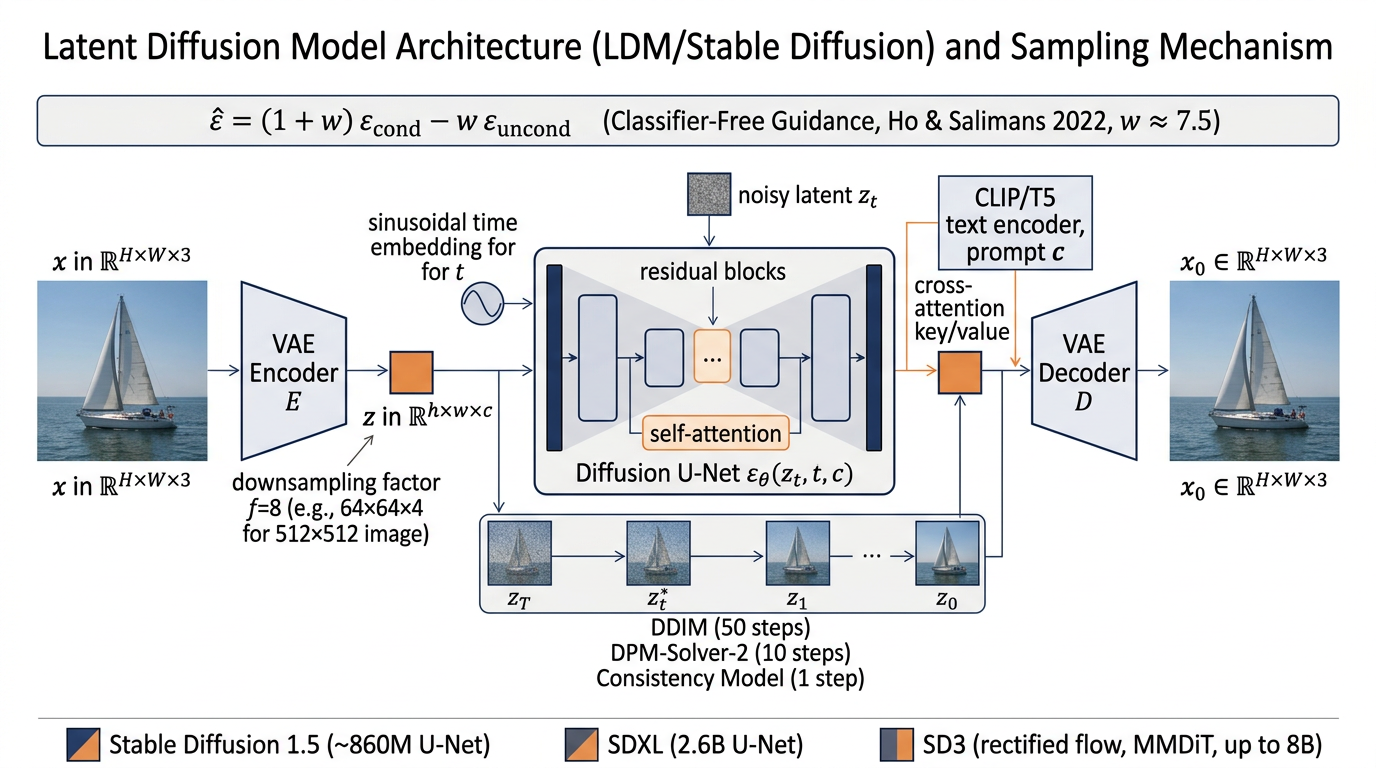
\includegraphics[keepaspectratio,alt={Latent diffusion architecture showing VAE encoder/decoder, U-Net with cross-attention, time embedding, and classifier-free guidance.}]{./figures/Generative-Diffusion-Models__fig3_ldm_architecture.png}}
\caption{Latent diffusion architecture showing VAE encoder/decoder, U-Net with cross-attention, time embedding, and classifier-free guidance.}
\end{figure}

Section 4 placed every method on a five-axis grid; this section zooms into the backbone axis and the conditioning modules layered on top, covering U-Net designs, DiT designs, latent autoencoders, conditioning modules, and time embeddings. The U-Net lineage runs from DDPM U-Net (2020, 36M on CIFAR-10) through ADM (2021, 553M with AdaGN), SD 1.5 U-Net (2022, 860M with cross-attention at every resolution), SD 2.1 U-Net (2022, OpenCLIP-H/14 conditioning), and SDXL U-Net (2023, 2.6B with two text encoders). The transformer lineage opens with DiT-XL/2 (2023, 675M with adaLN-Zero) and continues with PixArt-α (2024, 600M T5-conditioned DiT), PixArt-Σ (2024, 4K extension), MMDiT in SD3 (2024, up to 8B with shared text-image attention), and Sora's spatiotemporal-patch DiT (2024). Hybrid backbones include U-ViT (2022), DiffiT (2024, hybrid CNN-transformer), Diffusion Mamba (2024, bidirectional SSM), MaskDiT (2023, masked-token training), and EDM2 (2024, post-hoc EMA U-Net at FID 1.81 on ImageNet 512).

A diffusion backbone maps a noisy \(x_t\) to a prediction of ε, \(x_0\), v, or score, conditioned on timestep t and any auxiliary signal c.~Two architecture families dominate. Convolutional U-Nets carried 2020--2022 --- DDPM (\textasciitilde36M parameters on CIFAR-10), ADM (553M on ImageNet 256), Stable Diffusion 1.5 (860M U-Net + CLIP-L/14), SDXL (2.6B U-Net + OpenCLIP-bigG + CLIP-L), and the cascades of Imagen and DALL-E 2. Diffusion Transformers and their multimodal extensions have been the default at foundation scale since 2023 --- DiT-XL/2 (675M, ImageNet 256 FID 2.27), PixArt-α (\textasciitilde600M, \textasciitilde10× lower compute than SDXL for matched quality), MMDiT in SD3 (up to 8B parameters), and Sora's spatiotemporal-patch DiT. Failure modes are concrete: a weak autoencoder caps achievable quality regardless of backbone (one reason SD3 invested in a 16-channel KL-VAE over SDXL's 4-channel VAE, gaining \textasciitilde1.5 dB PSNR); a small text encoder caps prompt comprehension (replacing CLIP with T5-XXL drove Imagen's DrawBench preference up by \textasciitilde10 points); attention at fewer resolutions hurts long-range coherence in U-Nets and is one reason DiT scales more cleanly. The conditioning modules --- cross-attention, ControlNet, T2I-Adapter, IP-Adapter, DreamBooth, Textual Inversion, LoRA --- are orthogonal to backbone choice and ride on top to provide controllability.

\subsection{ADM-style U-Net design (Ho 2020, Dhariwal 2021)}\label{adm-style-u-net-design-ho-2020-dhariwal-2021}

Ho, Jain, and Abbeel's DDPM (2020) inherited a U-Net (Ronneberger et al.~2015) from PixelCNN++. The encoder--decoder shape with skip connections is well suited to denoising because the model must produce an output the same size as its input, and skip connections preserve high-frequency content that pure encoders would discard. DDPM used four resolution stages, two residual blocks per stage, group normalization, GeLU/SiLU activations, sinusoidal time embedding fed through a two-layer MLP and added to each residual block, and self-attention at the 16×16 stage. CIFAR-10 DDPM has roughly 36M parameters.

Dhariwal \& Nichol's \emph{Ablated Diffusion Model} (ADM, NeurIPS 2021) refined this design and scaled it. They added (i) larger width and depth (553M parameters at 256×256), (ii) attention at multiple resolutions (32, 16, 8), (iii) BigGAN-style residual block with a separate skip path, (iv) adaptive group normalization (AdaGN) injecting timestep and class embeddings as scale/shift, and (v) a learned variance head Σ\_θ for the reverse Gaussian. The resulting ImageNet 256×256 FID of 4.59 was the empirical proof that large U-Net diffusion beats GANs. ADM is the de-facto reference U-Net design that Stable Diffusion, GLIDE, and Imagen all closely follow.

Stable Diffusion 1.5 uses an ADM-style U-Net with cross-attention added at every resolution: each transformer block in the U-Net contains a self-attention, a cross-attention to text features (CLIP-ViT-L/14, 768-dim), and a feed-forward layer. The U-Net runs at 64×64 latent resolution (corresponding to 512×512 pixel input via the f=8 KL-VAE) and contains roughly 860M parameters. SDXL doubles the U-Net to 2.6B parameters, replaces the text conditioning with a concatenation of OpenCLIP-ViT-bigG/14 (1280-dim) and CLIP-ViT-L/14 (768-dim) features, and uses a stronger 4-channel VAE. SDXL also introduces \emph{micro-conditioning} on original image resolution, crop coordinates, and aspect ratio, so the model is aware of training-time crops. Pixel-space cascades (Imagen 64→256→1024, eDiff-I) use one U-Net per stage; the larger stages tend to be smaller and faster because they only learn detail enhancement.

\subsection{Diffusion Transformer (DiT, PixArt, MMDiT) and adaLN-Zero}\label{diffusion-transformer-dit-pixart-mmdit-and-adaln-zero}

Peebles \& Xie's \emph{Scalable Diffusion Models with Transformers} (DiT, ICCV 2023) replaced the U-Net entirely with a Vision-Transformer-style architecture. The latent (e.g., 32×32×4) is patchified into ViT tokens, processed by a stack of transformer blocks, and unpatchified to produce the prediction. Conditioning enters via \emph{adaLN-Zero}: a small MLP maps the timestep and class embeddings to scale/shift parameters that modulate each block's layer norm; crucially, the residual scales are initialized to zero so the network begins as identity, dramatically improving optimization stability. DiT-XL/2 (675M parameters, patch size 2) achieves FID 2.27 on ImageNet 256×256, beating ADM-G's 3.94 and approaching the contemporary GAN best of 2.0--2.5. DiT exhibits clean log-FID-vs-FLOPs scaling, making it the basis for foundation-scale T2I.

PixArt-α (Chen et al.~ICLR 2024) adapts DiT to text-to-image with cross-attention to T5-XXL features and demonstrates that \textasciitilde10× lower training compute than SDXL suffices for competitive generations on COCO and PartiPrompts. Pixart-Σ extends to 4K. \emph{MMDiT} (Multimodal Diffusion Transformer, Esser et al.~SD3 2024) processes image and text tokens jointly: each block has separate K/V/Q projections for the two modalities but shared attention over their concatenated tokens, allowing the model to learn token-level alignment. Stable Diffusion 3 uses MMDiT with up to 8B parameters and rectified-flow training. \emph{Sora} (OpenAI 2024) extends DiT to spatiotemporal patches: video is divided into patches in space and time, processed by a single transformer; conditioning includes text and a timestep, with the spatial-temporal aspect ratio also handled via micro-conditioning. \emph{DiT-3D} (Mo et al.~2023) and \emph{Direct3D} (Wu et al.~2024) apply DiT to 3D shape generation in voxel or latent-3D spaces.

DiT's advantages are (i) clean scaling laws shared with LLMs, (ii) freedom from convolutional inductive biases that do not transfer to non-image modalities, and (iii) flexible token-level conditioning. Disadvantages include slower inference at small scales (where U-Net's locality wins) and larger memory at very high resolutions.

\subsection{Latent autoencoders: VQ-GAN and KL-autoencoders for LDM/SDXL}\label{latent-autoencoders-vq-gan-and-kl-autoencoders-for-ldmsdxl}

Latent diffusion separates \emph{perceptual compression} (an autoencoder that maps pixels to latents) from \emph{semantic generation} (the diffusion model in latent space). Rombach et al.'s LDM uses two autoencoder variants: a VQ-GAN with a discrete codebook and a KL-regularized continuous-latent autoencoder. Stable Diffusion 1.5 uses the latter with downsampling factor f = 8 and 4 latent channels: a 512×512 RGB image becomes a 64×64×4 latent. SDXL retains f = 8 but trains a stronger 4-channel VAE with improved decoder; SD3 introduces a 16-channel KL-VAE that retains finer detail at 1024² and beyond. AudioLDM uses a mel-spectrogram autoencoder (HiFi-GAN-style decoder) so diffusion runs in mel-spectrogram latent space.

The autoencoder is trained with a perceptual loss (LPIPS), an adversarial loss (PatchGAN), and a KL or VQ regularizer. A weak autoencoder caps the achievable image quality regardless of the diffusion model --- when the decoder cannot represent fine text or hands, no T2I model trained over it can. This is one reason SD3 invested in a stronger 16-channel VAE.

\subsection{Cross-attention, ControlNet, T2I-Adapter, IP-Adapter}\label{cross-attention-controlnet-t2i-adapter-ip-adapter}

Conditioning enters a diffusion U-Net or DiT through cross-attention layers that compute attention from latent queries to keys/values produced by a frozen text encoder. CLIP-ViT-L/14 (Radford et al.~2021), OpenCLIP-ViT-G/14, and Google's T5-XXL (4.6B) are the typical text encoders. Imagen showed that scaling the \emph{text encoder} (T5-XXL) yields larger gains than scaling the U-Net, suggesting language understanding is the bottleneck for prompt comprehension.

\emph{ControlNet} (Zhang \& Agrawala, ICCV 2023) injects structural controls --- Canny edges, depth maps, segmentation maps, OpenPose skeletons, scribbles, normals --- into a frozen Stable Diffusion U-Net. ControlNet copies the U-Net's encoder, freezes the original, and connects them with zero-initialized 1×1 convolutions so training begins as identity. This allows the structural signal to refine generation without destroying the base model's prior. ControlNet on SD 1.5 became one of the most-used controllability tools, supporting \textgreater10 modalities of structural control. \emph{T2I-Adapter} (Mou et al.~AAAI 2024) is a lighter-weight alternative that injects features at the U-Net's encoder downsampling stages. \emph{IP-Adapter} lets a reference image act as a prompt by encoding it via CLIP-Image features and feeding them through a parallel cross-attention path.

\emph{DreamBooth} (Ruiz et al.~CVPR 2023) personalizes a diffusion model to a specific subject (e.g., a particular dog) by fine-tuning the full U-Net on 3--5 images of the subject with a class-prior preservation loss. The model learns an association between a rare token (e.g., ``{[}V{]} dog'') and the subject's identity. \emph{Textual Inversion} (Gal et al.~2022) instead freezes the U-Net and learns only a new token embedding to represent the subject. \emph{LoRA} (Low-Rank Adaptation; Hu et al.~2021) fine-tunes a low-rank decomposition of attention weight updates, producing personalization adapters of 5--50 MB that can be hot-swapped at inference. These methods enable consumer-grade personalization without retraining.

\subsection{Time embeddings and noise schedule conditioning}\label{time-embeddings-and-noise-schedule-conditioning}

Timestep t (or σ in EDM) is encoded via sinusoidal positional embeddings followed by a small MLP, producing a feature that is added to every residual block (U-Net) or used in adaLN-Zero (DiT). EDM uses log σ rather than t directly. Some recent systems use \emph{Min-SNR loss weighting} (Hang et al.~2023) which scales the per-timestep loss by min(γ, SNR(t)) for stability and convergence speed. The choice of γ ≈ 5 is empirically robust.

\subsection{Comparative architectural footprints}\label{comparative-architectural-footprints}

{\def\LTcaptype{none} % do not increment counter
\begin{longtable}[]{@{}
  >{\raggedright\arraybackslash}p{(\linewidth - 10\tabcolsep) * \real{0.2018}}
  >{\raggedright\arraybackslash}p{(\linewidth - 10\tabcolsep) * \real{0.1651}}
  >{\raggedright\arraybackslash}p{(\linewidth - 10\tabcolsep) * \real{0.1468}}
  >{\raggedright\arraybackslash}p{(\linewidth - 10\tabcolsep) * \real{0.1743}}
  >{\raggedright\arraybackslash}p{(\linewidth - 10\tabcolsep) * \real{0.1835}}
  >{\raggedright\arraybackslash}p{(\linewidth - 10\tabcolsep) * \real{0.1284}}@{}}
\toprule\noalign{}
\begin{minipage}[b]{\linewidth}\raggedright
System
\end{minipage} & \begin{minipage}[b]{\linewidth}\raggedright
Backbone
\end{minipage} & \begin{minipage}[b]{\linewidth}\raggedright
Backbone params
\end{minipage} & \begin{minipage}[b]{\linewidth}\raggedright
Latent shape
\end{minipage} & \begin{minipage}[b]{\linewidth}\raggedright
Text encoder
\end{minipage} & \begin{minipage}[b]{\linewidth}\raggedright
NFE typical
\end{minipage} \\
\midrule\noalign{}
\endhead
\bottomrule\noalign{}
\endlastfoot
DDPM (CIFAR-10) & U-Net & \textasciitilde36M & 32×32×3 (pixel) & none & 1000 \\
ADM-G (ImageNet 256) & Wide U-Net & \textasciitilde553M & 256×256×3 & class & 250 \\
GLIDE & U-Net & 3.5B + 1.5B & 64×64 → 256×256 & text-CLIP & 100 \\
Stable Diffusion 1.5 & U-Net & 860M & 64×64×4 & CLIP-L/14 & 50 \\
Stable Diffusion 2.1 & U-Net & 865M & 64×64×4 (768²) & OpenCLIP-H/14 & 50 \\
SDXL & U-Net & 2.6B & 128×128×4 (1024²) & OpenCLIP-G + CLIP-L & 50 \\
SD3 / MMDiT & MMDiT & 2B / 8B & 128×128×16 & T5-XXL + 2 CLIP & 28 (rectified) \\
Imagen & Cascade U-Net & 2B + 700M + 400M & 64²→256²→1024² & T5-XXL (4.6B) & 256 \\
DiT-XL/2 & Transformer & 675M & 32×32×4 & class & 250 \\
Pixart-α & DiT & 600M & 64×64×4 (512²) & T5-XXL & 50 \\
Sora (reported) & Spatiotemporal DiT & several B & space-time patches & text-encoder & undisclosed \\
Stable Video Diffusion & 3D U-Net & 1.5B & 8 frames × 72×128×4 & CLIP image embedding & 25 \\
AudioLDM & U-Net & 185M & mel-spec 256×16×8 & CLAP & 200 \\
RFdiffusion & RoseTTAFold + diff & \textasciitilde150M & residue graph & sequence/structure & 200 \\
\end{longtable}
}

\subsection{Hybrid and emerging backbones}\label{hybrid-and-emerging-backbones}

\emph{U-ViT} (Bao et al.~2022) keeps the U-shape but replaces convolution with transformer blocks. \emph{DiffiT} (Hatamizadeh et al.~ECCV 2024) introduces hybrid CNN--transformer blocks. \emph{Diffusion Mamba} (Mo \& Tian, 2024) uses bidirectional state-space models for sub-quadratic scaling on long video. \emph{MaskDiT} (Gao et al.~ICCV 2023) accelerates DiT training by masking out a subset of tokens during training, then unmasking at inference. \emph{EDM2} (Karras et al.~2024) further refines U-Net preconditioning with post-hoc EMA and achieves FID 1.81 on ImageNet 512.

\subsection{Why architectural choices matter empirically}\label{why-architectural-choices-matter-empirically}

Architectural choices stack measurably. ADM's adaptive group normalization improved ImageNet 256 FID by \textasciitilde0.3 over additive injection. DiT-XL/2 dropped ImageNet 256 FID from 4.59 (ADM-G) to 2.27 at similar parameter count. Switching CLIP to T5-XXL in Imagen improved DrawBench preference by \textasciitilde10 points, establishing text-encoder scale as the dominant T2I lever. SD3's 16-channel VAE improved reconstruction PSNR by \textasciitilde1.5 dB over SDXL's 4-channel VAE.

U-Nets dominate sub-foundation image diffusion and most video, audio, and 3D systems; DiT and MMDiT are the default at foundation scale, with conditioning modules layered on top. The next section turns to the loss functions that train them.

\section{Training Objectives and Optimization}\label{training-objectives-and-optimization}

This section turns to the loss functions, organized as the ELBO and \(L_s\)imple, v-prediction with EDM preconditioning, variational diffusion, flow matching, optimization details, and a comparison table. The objective lineage begins with Sohl-Dickstein et al.~(2015, original variational ELBO), DDPM \(L_s\)imple (2020, unweighted ε-MSE), and Improved DDPM \(L_h\)ybrid (2021, ELBO + \(L_s\)imple). Salimans \& Ho (2022) introduced v-prediction as a balanced parameterization, Karras (2022) added EDM preconditioning as σ-conditioned MSE, and Hang (2023) added Min-SNR weighting with γ ≈ 5. Variational Diffusion Models (Kingma 2021) reach CIFAR-10 NLL 2.49 bits/dim. The flow-matching family includes Flow Matching (Lipman 2023, vector-field regression), Rectified Flow (Liu 2023, iterated re-flow), and Stochastic Interpolants (Albergo 2023, unifying SDE+ODE). Post-training objectives include DPO-Diffusion (Wallace 2024, preference fine-tuning), DRaFT (Clark 2024, reward gradients), and DDPO (Black 2024, RL-style diffusion).

The training objective takes several mathematically equivalent or near-equivalent forms: the variational lower bound (ELBO), the simplified denoising loss \(L_s\)imple, weighted variants under EDM preconditioning, v-prediction (Salimans \& Ho 2022), the variational diffusion model bound (Kingma et al.~2021, CIFAR-10 NLL 2.49 bits/dim), and flow-matching / rectified-flow vector-field regression (Lipman et al.~ICLR 2023; Liu et al.~ICLR 2023). They differ measurably in stability, convergence speed, sample quality, and likelihood. DDPM, ADM, GLIDE, and Stable Diffusion 1.5 use ε-prediction with \(L_s\)imple. Imagen Video and SD 2.1 (v-mode) use v-prediction. EDM, EDM2, and many DiTs use preconditioned MSE. SD3, Lumina, and PixArt-Σ use rectified flow. Modern frontier systems combine these --- typically a noise-prediction variant of \(L_s\)imple plus EDM preconditioning plus Min-SNR weighting (γ ≈ 5; Hang et al.~2023) --- and increasingly migrate to flow matching at large scale. Each subsection documents one objective with its concrete benchmark anchor, optimizer setting, and known failure mode (NaN at low σ, mode collapse, watermark overfitting, memorization).

\subsection{The ELBO and the simplified noise loss}\label{the-elbo-and-the-simplified-noise-loss}

Sohl-Dickstein et al.~(2015) derived the variational lower bound: log p\emph{θ(\(x_0\)) ≥ −L = −\(E_q\){[}\(L_T\) + Σ\emph{\{t=2\}\^{}T L}\{t-1\} + \(L_0\){]}, where \(L_T\) = \(D_K\)L(q(\(x_T\)\textbar{}\(x_0\)) ‖ p(\(x_T\))) (constant if T large), L}\{t-1\} = D\emph{KL(q(x}\{t-1\}\textbar x\emph{t,\(x_0\)) ‖ p}θ(x\emph{\{t-1\}\textbar{}\(x_t\))) (the per-step denoising term), and \(L_0\) is the final reconstruction term. With ε-parameterization, L}\{t-1\} reduces to a weighted MSE between predicted and true noise, with weights involving β\_t and ᾱ\_t.

DDPM's central empirical finding is that \emph{removing the time-dependent weights} and using L\emph{simple = E}\{x\emph{0, ε, t\}{[}‖ε − ε\emph{θ(x}t, t)‖²{]} yields \_better} sample quality than the exact ELBO. The intuition is that the natural ELBO weights downweight low-noise (small t) terms --- exactly the terms responsible for fine detail. \(L_s\)imple flattens the weighting and biases learning toward perceptually important steps. Improved DDPM (Nichol \& Dhariwal 2021) introduced a hybrid loss \(L_h\)ybrid = \(L_s\)imple + λ \(L_v\)lb that re-introduces the variance head training while keeping \(L_s\)imple as the dominant term, enabling tight likelihood evaluation.

\subsection{v-prediction, EDM preconditioning, and Min-SNR weighting}\label{v-prediction-edm-preconditioning-and-min-snr-weighting}

Salimans \& Ho's \emph{v-prediction} parameterization, originally introduced in their 2022 progressive distillation paper, uses a target \(v_t\) = α\_t ε − σ\_t \(x_0\) (where α\_t = √ᾱ\_t and σ\_t = √(1−ᾱ\_t)). v-prediction is numerically better behaved at both the noise-dominated and signal-dominated extremes of the schedule, and it makes progressive distillation work across schedules. Stable Diffusion 2.1 (in its v-mode), Imagen Video, and many cascade super-resolution stages use v-prediction.

Karras et al.'s \emph{EDM} (NeurIPS 2022) treats the diffusion model as F\emph{θ(x; σ) --- a single function of x and σ --- with a }preconditioned* loss \(L_E\)DM = E\emph{\{σ, ε, x}0\}{[} λ(σ) ‖ D\emph{θ(x; σ) − x}0 ‖² {]}, where D\emph{θ(x; σ) = c}skip(σ) x + \(c_o\)ut(σ) F*θ(\(c_i\)n(σ) x, \(c_n\)oise(σ)) and the weighting λ(σ) is chosen so the loss has equal magnitude across noise levels. EDM preconditioning is now standard in both U-Net and DiT systems; it explains why some training runs converge dramatically faster than others without any change to architecture.

\emph{Min-SNR weighting} (Hang et al.~2023) further re-weights \(L_s\)imple by min(γ, SNR(t)) where SNR(t) = ᾱ\_t / (1 − ᾱ\_t) and γ ≈ 5. This downweights overly-easy low-noise steps and improves convergence; many SDXL-class systems use it implicitly.

\subsection{Variational diffusion models and continuous-time training}\label{variational-diffusion-models-and-continuous-time-training}

Kingma, Salimans, Poole, and Ho's \emph{Variational Diffusion Models} (NeurIPS 2021) showed that the discrete ELBO has a continuous-time limit equivalent to an integral over the signal-to-noise ratio. The continuous-time bound can be written L\emph{VDM = ½ E}\{x*0, ε, t\}{[} (SNR'(t)) ‖ε − ε*θ(\(x_t\), t)‖² {]}, where SNR' is the derivative of log SNR. By treating the noise schedule itself as a learnable function (subject to monotonicity), VDM achieves CIFAR-10 NLL of 2.49 bits/dim --- competitive with autoregressive PixelCNN++ and substantially better than earlier diffusion likelihoods. The VDM result also implies that two networks differing only in noise schedule but trained with the continuous-time bound can produce identical sample distributions --- schedule is no longer a confound.

\subsection{Flow matching, rectified flow, and stochastic interpolants}\label{flow-matching-rectified-flow-and-stochastic-interpolants}

Lipman, Chen, Ben-Hamu, Nickel, and Le's \emph{Flow Matching for Generative Modeling} (ICLR 2023) presents a simpler training paradigm. Define an interpolant x\emph{t = (1 − t) \(x_0\) + t \(x_1\) between data \(x_0\) \textasciitilde{} \(p_d\)ata and noise \(x_1\) \textasciitilde{} N(0, I). The }conditional vector field* connecting them is \(u_t\)(x \textbar{} \(x_0\), \(x_1\)) = \(x_1\) − \(x_0\) (the straight-line velocity). Train v\emph{θ(x, t) by L}CFM = E\emph{\{t, x}0, \(x_1\)\}{[} ‖ v\emph{θ(x}t, t) − (\(x_1\) − \(x_0\)) ‖² {]}. Sampling solves the ODE dx/dt = v*θ(x, t) from \(x_1\) to \(x_0\). This is mathematically a special case of stochastic interpolants (Albergo, Boffi, \& Vanden-Eijnden 2023) and a continuous-time relative of score matching.

Liu, Gong, \& Liu's \emph{Rectified Flow} (ICLR 2023) takes flow matching one step further: train, then \emph{re-flow} by retraining v\_θ on the model's own straight trajectories. Iterated re-flow makes the trajectories straight lines in expectation, allowing one-step or two-step generation while approximating the multi-step model's distribution. SD3 and Pixart-Σ adopt rectified flow at scale.

Albergo et al.'s \emph{Stochastic Interpolants} unify flow matching and score-based diffusion under a single framework. Setting σ\_t \textgreater{} 0 yields stochastic dynamics; σ\_t = 0 yields ODE flow. Schrödinger bridges (an optimal-transport viewpoint) emerge as a limiting case. This unification is theoretically clean and has practical value: a single codebase can train both diffusion and flow-matching variants by toggling σ.

\subsection{Optimization details}\label{optimization-details}

Training uses AdamW (Loshchilov \& Hutter 2019) with lr ≈ 1e-4 to 2e-4, β\_2 ∈ {[}0.95, 0.999{]}, weight decay \textasciitilde1e-2, and EMA decay 0.9999 for inference. Mixed-precision bf16 is standard at SDXL/SD3 scale. Effective batch sizes are 1024--4096. For LDM, the autoencoder is trained first and frozen. SDXL trained on LAION-aesthetics-v2-5+; SD3 used synthesized captions; RFdiffusion fine-tuned from RoseTTAFold.

\subsection{Data augmentation, classifier-free training, and curriculum}\label{data-augmentation-classifier-free-training-and-curriculum}

Most T2I systems use cropping and horizontal flipping. SDXL adds crop-coordinate conditioning to remove the ``zoomed-in'' bias. Imagen uses dynamic thresholding to clip CFG-induced overflows. Classifier-free guidance drops the prompt with probability \textasciitilde0.1 during training, training conditional and unconditional models jointly. Curriculum at scale (PixArt-α, SD3, Lumina-Next) trains at 256²/512² then fine-tunes at 1024² for compute efficiency.

\subsection{Comparison of training objectives}\label{comparison-of-training-objectives}

{\def\LTcaptype{none} % do not increment counter
\begin{longtable}[]{@{}
  >{\raggedright\arraybackslash}p{(\linewidth - 8\tabcolsep) * \real{0.1608}}
  >{\raggedright\arraybackslash}p{(\linewidth - 8\tabcolsep) * \real{0.1748}}
  >{\raggedright\arraybackslash}p{(\linewidth - 8\tabcolsep) * \real{0.1888}}
  >{\raggedright\arraybackslash}p{(\linewidth - 8\tabcolsep) * \real{0.2378}}
  >{\raggedright\arraybackslash}p{(\linewidth - 8\tabcolsep) * \real{0.2378}}@{}}
\toprule\noalign{}
\begin{minipage}[b]{\linewidth}\raggedright
Objective
\end{minipage} & \begin{minipage}[b]{\linewidth}\raggedright
Formula (sketch)
\end{minipage} & \begin{minipage}[b]{\linewidth}\raggedright
Used by
\end{minipage} & \begin{minipage}[b]{\linewidth}\raggedright
Pros
\end{minipage} & \begin{minipage}[b]{\linewidth}\raggedright
Cons
\end{minipage} \\
\midrule\noalign{}
\endhead
\bottomrule\noalign{}
\endlastfoot
ELBO & KL + reconstruction terms & Sohl-Dickstein 2015, VDM & Tight likelihood & Slower sample-quality convergence \\
L\_simple (ε-pred) & ‖ε − ε\_θ‖² & DDPM, ADM, GLIDE, SD 1.5 & Stable, simple & Suboptimal at extremes of schedule \\
x\_0-prediction & ‖x\emph{0 − x̂}θ‖² & Some segmentation & Works well at low SNR & Worse at high SNR \\
v-prediction & ‖v − v\_θ‖² & Imagen Video, SD 2.1 v-mode & Balanced, distillation-friendly & Requires schedule rewriting \\
EDM preconditioning & preconditioned MSE & EDM, EDM2, many DiTs & Best sample quality, schedule-free & More implementation complexity \\
Flow matching & ‖(x\emph{1 − x\_0) − v}θ‖² & SD3 base, Lumina, Pixart-Σ & Simpler, straight trajectories & Requires re-flow for 1-step \\
Rectified flow & iterated flow matching & SD3 (final) & 1-step capable & Multi-stage training \\
Stochastic interpolants & unified & Theoretical works & Generalizes both & Less battle-tested at scale \\
\end{longtable}
}

\subsection{Likelihood and density estimation}\label{likelihood-and-density-estimation}

Diffusion models permit exact likelihood via the probability-flow ODE. Score-SDE reports ImageNet 32 NLL 3.42 bits/dim; VDM achieves 2.49 on CIFAR-10. PixelCNN++ achieves \textasciitilde2.92, Image GPT \textasciitilde2.65. Diffusion now leads in both sample quality and likelihood.

\subsection{Failure modes during training}\label{failure-modes-during-training}

Common pathologies are: NaN losses at small noise (fixed by EDM preconditioning or clipping); mode collapse (fixed by larger batches or lower CFG drop probability); poor prompt comprehension (fixed by T5-XXL or CLIP-bigG); LAION-watermark overfitting (fixed by aesthetic scoring); and verbatim memorization (Carlini 2023; revisited in §12).

\subsection{Why progress on objectives matters}\label{why-progress-on-objectives-matters}

Diffusion's empirical history is largely a history of training-objective improvements. \(L_s\)imple (2020) made DDPM tractable. Cosine schedule + learned variance (2021) drove ImageNet-64 FID below 4. EDM preconditioning (2022) made 35-NFE sampling viable. Min-SNR weighting (2023) stabilized SDXL training at 2.6B parameters. Rectified flow (2024) made sub-30-step inference standard at 1024². Each innovation cost zero parameters but unlocked the next deployment frontier.

\section{Sampling, Acceleration, and Distillation}\label{sampling-acceleration-and-distillation}

This section reviews sampling and distillation, organized as ancestral / DDIM samplers, high-order ODE solvers, knowledge distillation, adversarial one-step generators, inverse-problem sampling, and a comparison table. DDPM ancestral (2020, 1000-step baseline) and DDIM (2021, 50-step deterministic) are the foundation. Higher-order ODE solvers include the Heun integrator in EDM (2022, 35 NFE at CIFAR-10 FID 1.79), DPM-Solver (2022, 10-NFE second-order), DPM-Solver++ (2023, CFG-aware), and UniPC (2023, 5--8-NFE predictor-corrector). Distillation runs in parallel: Progressive Distillation (Salimans \& Ho 2022, halving step count), Consistency Models (Song 2023, 1--4 NFE at CIFAR-10 FID 3.55), Latent Consistency Models (Luo 2023, 4-step SDXL), and LCM-LoRA (Luo 2023, universal 4-step adapter). Adversarial one-step generators include SDXL-Turbo / ADD (Sauer 2023, 1-step adversarial), Hyper-SD (2024, multi-stage distillation), and SD-Lightning (2024, fast 1024² inference). Rectified Flow 1-step (Liu 2023, iterated re-flow) and MAR (Li 2024, ImageNet 256 FID 1.55) close the few-step picture; inverse-problem samplers include DPS (Chung 2023, posterior sampling) and DDRM (Kawar 2022, SVD-based restoration).

A trained diffusion model is only useful if it samples efficiently. Naive DDPM ancestral sampling requires T = 1000 sequential network evaluations per image, intolerable for production. Sampling history therefore runs parallel to architecture history, with a clear NFE reduction trajectory: 1000 (DDPM 2020) → 50 (DDIM 2021) → 35 (EDM Heun 2022) → 10 (DPM-Solver-2 2022) → 5--8 (UniPC 2023) → 1--4 (Consistency Models 2023, LCM 2023, SDXL-Turbo 2023). At 1024×1024 SDXL on a single A100, this collapses \textasciitilde30 seconds of inference into well under one second. We organize the techniques into four families: (i) deterministic non-Markovian samplers (DDIM); (ii) high-order ODE solvers exploiting the linear-Gaussian structure of the diffusion ODE (Heun, DPM-Solver, DPM-Solver++, UniPC); (iii) knowledge distillation into few-step students (progressive distillation, consistency models, LCM, LCM-LoRA); and (iv) adversarial distillation into one-step students (SDXL-Turbo / ADD, Hyper-SD, Lightning). Each family has its own quality--speed tradeoff: DPM-Solver++ matches DDIM-50 quality at 20 NFE, LCM matches the SDXL teacher within \textasciitilde5\% at 4 NFE, SDXL-Turbo matches within \textasciitilde10\% at 1 NFE. The remaining gap is concentrated in compositional binding under high CFG and in small-text rendering --- failure modes that multi-step CFG masks but few-step students expose.

\subsection{Ancestral sampling and DDIM}\label{ancestral-sampling-and-ddim}

DDPM's \emph{ancestral sampler} draws x\emph{T \textasciitilde{} N(0, I) and iterates x}\{t-1\} \textasciitilde{} N(μ\emph{θ(\(x_t\), t), Σ}θ(\(x_t\), t)) for t = T, T−1, \ldots, 1. With T = 1000 this produces high-quality samples but takes minutes per image on a single A100. Two main strategies for acceleration emerged.

Jiaming Song, Chenlin Meng, and Stefano Ermon's \emph{Denoising Diffusion Implicit Models} (DDIM, ICLR 2021) observed that the marginals q(x\emph{t \textbar{} \(x_0\)) --- and therefore the model's training --- depend only on the per-step variance schedule, not on the underlying chain's Markov structure. They constructed a non-Markovian generative process matching the same marginals but admitting a deterministic update x}\{t-1\} = √(ᾱ*\{t-1\}) x̂\_0(\(x_t\)) + √(1 − ᾱ\emph{\{t-1\}) ε}θ(\(x_t\), t), where x̂\_0 is recovered from \(x_t\) and ε*θ. With η = 0 the sampler is deterministic; with η = 1 it reduces to DDPM ancestral. Importantly, DDIM permits \emph{time skipping} --- taking 50 evenly spaced steps from T = 1000 --- with only minor sample-quality loss. DDIM with 50 steps became the de-facto baseline for inference and is what Stable Diffusion ships with by default.

\subsection{ODE/SDE solvers: Heun, DPM-Solver, DPM-Solver++, UniPC}\label{odesde-solvers-heun-dpm-solver-dpm-solver-unipc}

Treating the probability-flow ODE as a stiff differential equation invites classical numerical methods. Karras et al.'s EDM (NeurIPS 2022) uses \emph{Heun's second-order method} --- a predictor-corrector that combines forward Euler with a midpoint correction --- and reports CIFAR-10 FID 1.79 with only 35 NFE. The Heun integrator is now the EDM default.

Cheng Lu, Yuhao Zhou, Fan Bao, Jianfei Chen, Chongxuan Li, and Jun Zhu's \emph{DPM-Solver} (NeurIPS 2022) exploits the linear-Gaussian structure of the diffusion ODE. They derive a closed-form integrating-factor expansion that permits second- and third-order updates with very few NFE. DPM-Solver-2 reaches near-converged FID at NFE = 10, and DPM-Solver-3 at NFE = 12. \emph{DPM-Solver++} (Lu et al.~2023) extends this to guided sampling (CFG \textgreater{} 5), and \emph{UniPC} (Zhao et al.~2023) is a multi-step predictor-corrector that further reduces NFE to \textasciitilde5--8 for SDXL-class models. By 2024 DPM-Solver++ is the default sampler in many production T2I systems, including diffusers' default for SDXL.

\subsection{Knowledge distillation: progressive distillation, consistency models, LCM}\label{knowledge-distillation-progressive-distillation-consistency-models-lcm}

When the underlying ODE/SDE is too complex for analytical solvers, knowledge distillation can compress a multi-step teacher into a few-step student.

\emph{Progressive distillation} (Salimans \& Ho, ICLR 2022) recursively halves the step count: a student is trained to match the teacher's two-step output in one step, then the resulting model becomes the teacher for the next halving. Starting from a 1000-step DDPM, eight rounds of distillation yields a strong 4-step model, then a 2-step model, then a 1-step model. v-prediction is essential because ε-prediction destabilizes at very low NFE.

Yang Song, Prafulla Dhariwal, Mark Chen, and Ilya Sutskever's \emph{Consistency Models} (ICML 2023) train a function f\emph{θ(\(x_t\), t) → \(x_0\) such that f is }self-consistent* across timesteps: f\emph{θ(x}t, t) = f*θ(x\_\{t'\}, t') for any pair on the same diffusion trajectory. Two training modes exist: \emph{consistency distillation} from a pre-trained diffusion teacher and \emph{consistency training} from scratch. CIFAR-10 consistency models achieve FID 3.55 with 1 NFE and 2.93 with 2 NFE. \emph{Latent Consistency Models} (Luo et al.~2023) distill Stable Diffusion / SDXL into a 2--4 step generator at 1024² resolution. \emph{LCM-LoRA} (Luo et al.~2023) distills only the LoRA adapters, producing a universal 4-step accelerator that can be plugged into any SD variant.

\emph{Adversarial distillation} (StyleGAN-T 2023, SDXL-Turbo / ADD by Sauer et al.~2023) trains a one-step student against a discriminator. SDXL-Turbo generates 512² images in \textasciitilde150 ms on an A100 --- fast enough for real-time sketching interfaces. \emph{Streamlined Diffusion} and \emph{Lightning models} extend this further. Adversarial distillation can match teacher quality at the cost of training instability and \textasciitilde10--30\% drop on prompt comprehension benchmarks.

\subsection{One-step generators and adversarial distillation (SDXL-Turbo, ADD, MAR)}\label{one-step-generators-and-adversarial-distillation-sdxl-turbo-add-mar}

By 2024--2026, one-step generators have closed much of the quality gap with multi-step diffusion. SDXL-Turbo, Stable Diffusion XL Lightning, Hyper-SD, and PixArt-LCM each produce 1024² images in well under one second on consumer GPUs. The remaining gap is primarily in compositional binding and small-text rendering, which CFG and many sampling steps mask in the teacher but exposed in the student.

A complementary line is \emph{masked autoregressive generation} (MAR; Li et al.~2024) which combines diffusion-style continuous-space prediction with autoregressive sequence modeling --- generating image tokens in random order with a small per-token diffusion head. MAR achieves FID 1.55 on ImageNet 256 at high throughput, and is increasingly seen as a foundation-model-friendly alternative to per-image diffusion.

\subsection{Sampler comparison}\label{sampler-comparison}

{\def\LTcaptype{none} % do not increment counter
\begin{longtable}[]{@{}
  >{\raggedright\arraybackslash}p{(\linewidth - 6\tabcolsep) * \real{0.2706}}
  >{\raggedright\arraybackslash}p{(\linewidth - 6\tabcolsep) * \real{0.1294}}
  >{\raggedright\arraybackslash}p{(\linewidth - 6\tabcolsep) * \real{0.3176}}
  >{\raggedright\arraybackslash}p{(\linewidth - 6\tabcolsep) * \real{0.2824}}@{}}
\toprule\noalign{}
\begin{minipage}[b]{\linewidth}\raggedright
Sampler
\end{minipage} & \begin{minipage}[b]{\linewidth}\raggedright
NFE typical
\end{minipage} & \begin{minipage}[b]{\linewidth}\raggedright
Image FID (ImageNet 256)
\end{minipage} & \begin{minipage}[b]{\linewidth}\raggedright
Notes
\end{minipage} \\
\midrule\noalign{}
\endhead
\bottomrule\noalign{}
\endlastfoot
DDPM ancestral & 1000 & 4.59 (ADM) & Baseline \\
DDIM & 50 & 4.62 (ADM) & Deterministic, time-skip \\
Heun (EDM) & 35 & 1.79 (CIFAR-10) & Predictor-corrector \\
DPM-Solver-2 & 10 & \textasciitilde5.0 (ADM) & Closed-form ODE \\
DPM-Solver-3 & 12 & \textasciitilde4.9 (ADM) & Higher order \\
DPM-Solver++ (2M) & 20 & \textasciitilde4.8 (SDXL @ 1024) & Default in many T2I \\
UniPC & 5--8 & comparable & Predictor-corrector \\
Consistency Model (CD) & 1 & 3.55 (CIFAR-10) & Distilled from teacher \\
Consistency Model (CD) & 2 & 2.93 (CIFAR-10) & \\
LCM (SDXL) & 4 & matches teacher within \textasciitilde5\% & Distillation \\
SDXL-Turbo / ADD & 1 & matches teacher within \textasciitilde10\% & Adversarial distillation \\
Rectified Flow (SD3) & 28 & SOTA on T2I-CompBench & Straight trajectories \\
Rectified Flow (1-step) & 1 & comparable to LCM & Iterated re-flow \\
\end{longtable}
}

\subsection{Memory, throughput, and engineering}\label{memory-throughput-and-engineering}

Inference memory is dominated by attention activations. SDXL at 1024² needs \textasciitilde7 GB VRAM at batch 1; SD3 at 1024² needs \textasciitilde12 GB. Token merging (ToMe, Bolya 2023), xFormers / Flash-Attention, 8-bit/4-bit quantization, and distillation onto small backbones (Pixart-LCM 600M) compound for \textasciitilde10× throughput. H100 with TensorRT and FP8 reaches \textgreater100 SDXL images per second per node.

\subsection{Sample-quality vs.~step-count tradeoffs}\label{sample-quality-vs.-step-count-tradeoffs}

The FID-vs-NFE curve has three regimes. NFE ≥ 100: converged. NFE ∈ {[}10, 100{]}: smooth degradation. NFE ∈ \{1, 2, 4\}: only distilled or rectified-flow students approach teacher quality. CFG and NFE interact strongly; high CFG (w = 12) at low NFE (4) saturates outputs; DPM-Solver++ (Lu 2023) provides CFG-aware variants.

\subsection{Inverse problem solvers as samplers}\label{inverse-problem-solvers-as-samplers}

A branch of sampling treats diffusion as a prior for inverse problems. DPS (Chung 2023) adds a likelihood-gradient term ∇\_x log p(y \textbar{} x) via a differentiable forward operator A. DDRM (Kawar 2022) uses SVD decomposition. MCG, ΠGDM, RED-diff, and GDP are variants, with state-of-the-art MRI super-resolution and sparse-view CT (Singh 2024; Wu 2024).

\subsection{Why sampling acceleration matters}\label{why-sampling-acceleration-matters}

Deployment economics scale with NFE × per-step compute. Compressing NFE from 1000 to 4 via consistency distillation cuts per-image compute by \textasciitilde250×, comparable to two GPU generations. This makes real-time 1024² generation commercially viable in 2024--2026 and enables new categories: game asset generation, avatar puppeting, and low-latency robot policy execution (Consistency Policy, RSS 2024).

{\def\LTcaptype{none} % do not increment counter
\begin{longtable}[]{@{}
  >{\raggedright\arraybackslash}p{(\linewidth - 6\tabcolsep) * \real{0.4627}}
  >{\raggedright\arraybackslash}p{(\linewidth - 6\tabcolsep) * \real{0.2985}}
  >{\raggedright\arraybackslash}p{(\linewidth - 6\tabcolsep) * \real{0.1791}}
  >{\raggedright\arraybackslash}p{(\linewidth - 6\tabcolsep) * \real{0.0597}}@{}}
\toprule\noalign{}
\begin{minipage}[b]{\linewidth}\raggedright
Acceleration family
\end{minipage} & \begin{minipage}[b]{\linewidth}\raggedright
Speedup vs DDPM-1000
\end{minipage} & \begin{minipage}[b]{\linewidth}\raggedright
Quality cost
\end{minipage} & \begin{minipage}[b]{\linewidth}\raggedright
Year
\end{minipage} \\
\midrule\noalign{}
\endhead
\bottomrule\noalign{}
\endlastfoot
DDIM 50-step & 20× & minor & 2021 \\
EDM Heun 35-step & \textasciitilde28× & none & 2022 \\
DPM-Solver-2 (10 NFE) & 100× & small & 2022 \\
Progressive distillation 4-step & 250× & small & 2022 \\
Consistency models (1 NFE) & 1000× & moderate & 2023 \\
LCM (4 NFE on SDXL) & 12.5× vs DDIM-50 & moderate & 2023 \\
SDXL-Turbo / ADD (1 NFE) & 50× vs DDIM-50 & moderate & 2023 \\
Rectified Flow (28 NFE) & \textasciitilde36× & none & 2024 \\
Rectified Flow 1-step & 1000× & moderate & 2024 \\
\end{longtable}
}

Sampling and distillation are now central to deployment. The combination of (a) high-order ODE solvers, (b) consistency-model distillation, (c) latent-space inference, and (d) hardware-aware quantization has cut the cost of a high-resolution image from 30+ seconds in 2021 to under 1 second in 2024 --- a 30× wall-clock improvement that has doubled annually. The next frontier, sub-100 ms 1080p video, is plausible by 2026 with further work on rectified-flow distillation and DiT-Mamba-style sub-quadratic attention. The next section turns from how to \emph{sample} a diffusion model to how to \emph{control} it through conditioning and guidance.

\section{Conditioning, Guidance, and Controllability}\label{conditioning-guidance-and-controllability}

This section reviews conditioning, guidance, and controllability, organized as classifier and classifier-free guidance, structural ControlNet-family conditioning, personalization adapters, and editing methods. Dhariwal \& Nichol (2021) introduced classifier guidance via gradient-based class steering, and Ho \& Salimans (2022) proposed classifier-free guidance via drop-probability training. Ahn (2024) added Perturbed-Attention Guidance, Chung (2024) introduced manifold-constrained CFG++, and Hong (2022) proposed Self-Attention Guidance. Structural conditioning includes ControlNet (Zhang \& Agrawala 2023, edges/depth/pose), T2I-Adapter (Mou 2024, lightweight adapters), IP-Adapter (Ye 2023, image-prompt cross-attention), GLIGEN (Li 2023, region-grounded), and Composer (2023, multi-condition fusion). Personalization adapters include DreamBooth (Ruiz 2023, full-model personalization), Textual Inversion (Gal 2023, token-embedding learning), LoRA (Hu 2022, low-rank adapters), and Custom Diffusion (Kumari 2023, K/V fine-tuning). Editing methods include SDEdit (Meng 2022, partial-noise editing), Prompt-to-Prompt (Hertz 2023, attention-map editing), Null-Text Inversion (Mokady 2023, real-image editing), InstructPix2Pix (Brooks 2023, instruction-following editor), Imagen Editor (Wang 2022, mask-based editing), and RePaint (Lugmayr 2022, inpainting).

A defining strength of diffusion is the breadth of mechanisms by which user intent enters the sampling process. Conditioning ranges from coarse class labels (ImageNet, ADM-G) through free-form text (Stable Diffusion, DALL-E 3, Imagen, SD3), structural constraints (Canny edges, depth, OpenPose, segmentation, scribbles, normals via ControlNet), reference images (IP-Adapter, BLIP-Diffusion), audio (AudioLDM), motion fields, and partial observations (inpainting via RePaint, MAT, Imagen Editor). On top of conditioning sit \emph{guidance} methods --- classifier guidance (Dhariwal \& Nichol 2021) and classifier-free guidance (Ho \& Salimans, July 2022) --- that amplify the model's response to the condition during sampling. CFG drop probability \textasciitilde0.1 during training is what makes the inference-time linear combination ε̂ = (1 + w) ε\emph{θ(c) − w ε}θ(∅) work; typical w ≈ 3 (balanced) to 7.5 (strong adherence) for SD, with w \textgreater{} 12 producing oversaturation artifacts. The four principal axes documented below are: classifier-free guidance, structural conditioning (ControlNet, T2I-Adapter, IP-Adapter), personalization (DreamBooth, Textual Inversion, LoRA, Custom Diffusion), and editing (SDEdit, Prompt-to-Prompt, InstructPix2Pix, RePaint).

\subsection{Classifier guidance and classifier-free guidance (CFG)}\label{classifier-guidance-and-classifier-free-guidance-cfg}

\emph{Classifier guidance} (Dhariwal \& Nichol, NeurIPS 2021) modifies the reverse-time SDE with the gradient of an auxiliary noise-aware classifier p\emph{φ(y \textbar{} \(x_t\)): the score s}θ(x\emph{t, t) is replaced with s}θ(x\emph{t, t) + γ ∇}\{x\emph{t\} log p}φ(y \textbar{} \(x_t\)), where γ is the guidance scale. Larger γ pushes samples further along the class direction at the cost of diversity. Classifier guidance gave ADM its ImageNet 256 FID 4.59 result. The approach requires training a separate noisy classifier --- an extra model and training pipeline.

Jonathan Ho and Tim Salimans's \emph{Classifier-Free Diffusion Guidance} (CFG, July 2022) eliminated this overhead. During training, the prompt is dropped (replaced with empty / null) with probability \textasciitilde0.1, training one network to model both p(x \textbar{} c) and p(x). At inference, the predictions are combined as ε̂ = (1 + w) ε\emph{θ(\(x_t\), t, c) − w ε}θ(\(x_t\), t, ∅), where w is the guidance scale. CFG gives the same diversity-fidelity tradeoff as classifier guidance without the auxiliary model. Typical values are w ≈ 3 (balanced) to 7.5 (strong adherence) for Stable Diffusion; very large w \textgreater{} 12 produces oversaturated, posterized outputs.

CFG is universal: it appears in essentially every text-conditional diffusion system (GLIDE, DALL-E 2, Imagen, Stable Diffusion 1.5/2.1/XL/3, Pixart-α, Sora). Recent research has tried to fix CFG's known artifacts. \emph{Perturbed-Attention Guidance} (PAG; Ahn et al.~2024) replaces the unconditional prediction with one computed by perturbing self-attention. \emph{CFG++} (Chung et al.~2024) provides manifold-constrained CFG that preserves DDIM invertibility. \emph{Self-Attention Guidance} (Hong et al.~2022) and \emph{Token Perturbation Guidance} (2025) further refine the basic CFG mechanism. \emph{Annealing Guidance Scale} (2025) varies w over the trajectory rather than holding it fixed.

\subsection{ControlNet, T2I-Adapter, and structural conditioning}\label{controlnet-t2i-adapter-and-structural-conditioning}

Free-form text alone cannot pin down geometry: where the subject's hands go, the angle of a chair, the road perspective. Lvmin Zhang and Maneesh Agrawala's \emph{ControlNet} (ICCV 2023) addresses this by learning a \emph{trainable copy} of Stable Diffusion's encoder blocks that takes a structural input (Canny edges, depth maps, segmentation masks, OpenPose skeletons, scribbles, normal maps, MLSD lines, ADE20K segmentation) and injects features into the frozen base U-Net via zero-initialized 1×1 convolutions. Because the connections start at zero, training begins as the identity, preserving the base model's prior. ControlNet quickly grew to support 10+ conditioning modalities and is one of the most-downloaded models on Hugging Face.

\emph{T2I-Adapter} (Mou et al.~AAAI 2024) is a lighter-weight alternative: small adapter modules (\textasciitilde70M parameters vs.~ControlNet's full encoder copy) feed structural information into the U-Net's encoder downsampling stages. T2I-Adapter trades some fidelity for \textasciitilde3× faster training and inference. \emph{IP-Adapter} (Ye et al.~2023) lets a \emph{reference image} act as the prompt: a CLIP-Image encoder produces an embedding that conditions a parallel cross-attention path. IP-Adapter is widely used for style transfer and reference-driven generation.

Other structural conditioning tools include \emph{GLIGEN} (region-grounded generation), \emph{Composer}, \emph{MultiControlNet} (combining several ControlNets), and \emph{Uni-ControlNet}. They are all variations of the same theme: inject auxiliary signals through frozen-base + trainable-adapter architectures.

\subsection{Personalization: DreamBooth, Textual Inversion, LoRA, Custom Diffusion}\label{personalization-dreambooth-textual-inversion-lora-custom-diffusion}

Personalization adapts a pre-trained T2I model to a specific subject (a particular dog, person, object) or style (a particular artist's brushwork) using just 3--10 reference images. The four main methods are:

\emph{DreamBooth} (Ruiz et al.~CVPR 2023) fine-tunes the entire U-Net with two terms: a reconstruction loss on the subject images using a rare token ``{[}V{]}'' and a \emph{class-specific prior preservation loss} on generic class examples to prevent the model from forgetting the broader category. DreamBooth produces high-quality identity preservation but requires storing the full fine-tuned model (\textasciitilde860 MB for SD 1.5).

\emph{Textual Inversion} (Gal et al.~ICLR 2023) freezes the entire U-Net and learns \emph{only} a new token embedding (typically 1024-dimensional) that represents the subject. This produces a tiny artifact (\textasciitilde4 KB per concept) but with weaker identity fidelity than DreamBooth.

\emph{LoRA} (Hu et al.~ICLR 2022; adapted to diffusion by simo-ryu and the Stable Diffusion community in 2023) decomposes attention weight updates into a product of low-rank matrices A and B (rank typically 4--32) and trains only A, B. The resulting LoRA adapter is 5--50 MB, can be merged into the base weights at inference, and can be combined with multiple LoRAs (style + subject) at varying strengths. LoRA has become the dominant personalization format on civit.ai and similar communities, with millions of public LoRAs available.

\emph{Custom Diffusion} (Kumari et al.~CVPR 2023) restricts fine-tuning to the cross-attention K, V projections, achieving DreamBooth-comparable quality with \textasciitilde3\% of the parameters trained.

\subsection{Editing: SDEdit, Prompt-to-Prompt, InstructPix2Pix, RePaint, Imagen Editor}\label{editing-sdedit-prompt-to-prompt-instructpix2pix-repaint-imagen-editor}

Image editing applies a learned diffusion prior to modify existing images.

Chenlin Meng, Yutong He, Yang Song et al.'s \emph{SDEdit} (ICLR 2022) takes a user image, adds noise to time t* (typically halfway through the schedule), and runs the reverse process. The result preserves global structure while gaining synthesis-quality details. SDEdit can apply a target style or manipulate based on hand-drawn strokes.

\emph{Prompt-to-Prompt} (Hertz et al.~ICLR 2023) edits via cross-attention map manipulation: it replaces, reweights, or extends the cross-attention at each layer to swap or modify objects without changing the image's structure. \emph{Null-text Inversion} (Mokady et al.~2023) makes Prompt-to-Prompt work on real images by inverting them through DDIM and re-running with edited prompts.

\emph{InstructPix2Pix} (Brooks, Holynski, \& Efros, CVPR 2023) trains a Stable Diffusion variant on paired (image, text-instruction, edited-image) tuples synthesized via GPT-3 + Prompt-to-Prompt. The result is a one-shot instruction-following editor: given an image and ``make it night,'' it returns the night version. \emph{Imagen Editor} (Wang et al.~2022) and \emph{EditBench} benchmarked text-guided inpainting at scale.

\emph{RePaint} (Lugmayr et al.~CVPR 2022) does inpainting by re-noising the unmasked regions to match the model's reverse trajectory at each step, enabling consistent inpainting. \emph{BLIP-Diffusion}, \emph{AnyDoor}, \emph{Paint-by-Example}, and \emph{Paint-by-Word} extend this to subject-driven inpainting.

\subsection{Multi-condition fusion}\label{multi-condition-fusion}

Production systems combine text + ControlNet (depth) + IP-Adapter (style) + LoRA (subject). Composition is additive in cross-attention space; conflicting conditions are handled with per-condition guidance scales and learned routing (MoEController; Li 2023).

\subsection{Concept erasure and unlearning}\label{concept-erasure-and-unlearning}

Erasing Concepts from Diffusion Models (Gandikota 2023), Erasing Undesirable Influence (Wu 2024), and Selective Amnesia fine-tune models to suppress target concepts (celebrity faces, copyrighted characters, NSFW). Red-teaming work shows residual recoverability via adversarial prompts; these techniques form the basis of compliance pipelines.

\subsection{Conditioning summary}\label{conditioning-summary}

{\def\LTcaptype{none} % do not increment counter
\begin{longtable}[]{@{}
  >{\raggedright\arraybackslash}p{(\linewidth - 6\tabcolsep) * \real{0.2353}}
  >{\raggedright\arraybackslash}p{(\linewidth - 6\tabcolsep) * \real{0.2059}}
  >{\raggedright\arraybackslash}p{(\linewidth - 6\tabcolsep) * \real{0.3235}}
  >{\raggedright\arraybackslash}p{(\linewidth - 6\tabcolsep) * \real{0.2353}}@{}}
\toprule\noalign{}
\begin{minipage}[b]{\linewidth}\raggedright
Mechanism
\end{minipage} & \begin{minipage}[b]{\linewidth}\raggedright
What it conditions on
\end{minipage} & \begin{minipage}[b]{\linewidth}\raggedright
Method
\end{minipage} & \begin{minipage}[b]{\linewidth}\raggedright
Inference overhead
\end{minipage} \\
\midrule\noalign{}
\endhead
\bottomrule\noalign{}
\endlastfoot
Classifier guidance & class label & gradient of noisy classifier & extra classifier forward \\
Classifier-free guidance & text/class & drop probability + linear combine & 2× forwards \\
ControlNet & edges/depth/pose/seg & trainable encoder copy & +1 encoder forward \\
T2I-Adapter & structural & lightweight adapters & small overhead \\
IP-Adapter & reference image & parallel cross-attention & small overhead \\
DreamBooth & subject identity & full fine-tuning & none at inference \\
Textual Inversion & subject identity & new token embedding & none \\
LoRA & subject / style & low-rank adapters & none after merge \\
Custom Diffusion & subject & cross-attn K/V fine-tune & none \\
SDEdit & sketch / image & partial-noise re-sampling & reduced steps \\
Prompt-to-Prompt & text edit & cross-attn manipulation & per-step routing \\
InstructPix2Pix & text instruction & trained editor & none \\
RePaint & mask & re-noise unmasked region & iterative \\
Concept Erasure & unwanted concept & fine-tuning & none \\
\end{longtable}
}

\subsection{Why conditioning research dominates the practical literature}\label{why-conditioning-research-dominates-the-practical-literature}

Conditioning is the value layer of diffusion. Every commercial T2I product (Midjourney v6, DALL-E 3, Adobe Firefly, Ideogram, Recraft) competes on conditioning fidelity, prompt comprehension, and personalization. RFdiffusion conditions on protein constraints; Diffusion Policy conditions on robot observations; DPS conditions on medical measurements. Two trends dominate 2025--2026: unification of conditioning into a single MMDiT-style token interface, and provenance tagging that propagates through outputs.

\section{Modality-Specific Diffusion: Images, Video, Audio, 3D, and Beyond}\label{modality-specific-diffusion-images-video-audio-3d-and-beyond}

This section reviews how diffusion is deployed across modalities --- image, video, audio, 3D, motion, discrete data, and time series --- with a flagship table per modality. Image systems include Stable Diffusion 3 (2024), Imagen (2022), DALL-E 3 (2023), SDXL (2023), Pixart-α (2024), Flux (2024), SR3 (2022, super-resolution), and Palette (2022, image-to-image). Video systems include Imagen Video (2022), Make-A-Video (2022), VideoLDM (2023), Stable Video Diffusion (2023), Sora (2024), Lumiere (2024), and W.A.L.T (2023). Audio includes AudioLDM (2023), MusicLDM (2024), Noise2Music (2023), DiffWave (2021), WaveGrad (2021), Grad-TTS (2021, TTS), and DiffSinger (2022, singing). 3D systems include DreamFusion (2023), Magic3D (2023), Zero-1-to-3 (2023), MVDream (2023), CLAY (2024, asset-quality), and Hunyuan3D 2.0 (2025); MDM (2023) anchors human motion. Discrete-data systems include Diffusion-LM (2022, text), D3PM (2021), and SEDD (2024). Time-series and tabular work includes TimeGrad (2021), CSDI (2021, imputation), and TabDDPM (2023).

Generative diffusion is now deployed across every modality with structured data. This section surveys flagship systems by modality with their architecture, training corpus, and headline metric. Image: SDXL (2.6B U-Net, LAION-aesthetics, 1024², CLIP-Score competitive on PartiPrompts), SD3/MMDiT (8B, T5-XXL, leading T2I-CompBench), DALL-E 2 (COCO-30K FID 10.39), Imagen (FID 7.27), SR3 (FFHQ super-resolution PSNR/LPIPS leader). Video: Imagen Video (Kinetics-600 FVD \textasciitilde70), Stable Video Diffusion (1.5B, 152M curated clips, 1024×576), Sora (60-second 1080p with spatiotemporal-patch DiT). Audio: AudioLDM (AudioSet FAD 1.97), Grad-TTS (LJSpeech MOS 4.4+), DiffWave / WaveGrad vocoders, Noise2Music (MusicCaps), DiffSinger (singing voice synthesis). 3D: DreamFusion / ProlificDreamer (text-to-3D via SDS), Zero-1-to-3 (image-to-3D), CLAY / Hunyuan3D (asset-quality), DiT-3D and Direct3D (DiT in 3D space). Motion: MDM (HumanML3D R-Precision 0.78+). Discrete: Diffusion-LM, D3PM, SEDD. Time series: TimeGrad, CSDI. The goal is that a query like ``state-of-the-art audio diffusion?'' or ``how does Sora handle long video?'' lands directly in the relevant subsection with a citation, dataset size, and metric. Common failure modes --- temporal incoherence in long video, the multi-view ``Janus problem'' in 3D, lyrics-music alignment in long-form music, and out-of-distribution generalization in robotics --- are flagged where they apply.

\subsection{Image generation and editing}\label{image-generation-and-editing}

Image generation is the modality where diffusion first achieved dominance. The market is segmented into \emph{foundation T2I models} (DALL-E, Imagen, Stable Diffusion, Pixart, Flux, Lumina), \emph{editing tools} (InstructPix2Pix, Imagen Editor, EditBench), and \emph{super-resolution / restoration} (SR3, ESRGAN-Diff, Pixel-Aware SD, GFPGAN-Diff).

\emph{Stable Diffusion 1.5} (Rombach et al.~2022, released by Stability AI October 2022) is an 860M-parameter U-Net latent diffusion at 512×512, trained on LAION-aesthetics-v2-5+ for \textasciitilde150K A100-GPU-hours. Zero-shot COCO-30K FID ≈ 12.6 with CFG = 3. Despite its age, SD 1.5 remains the workhorse base model for the open-source community because of its compatibility with thousands of LoRAs and ControlNets.

\emph{Stable Diffusion XL} (Podell et al.~arXiv 2023) is 2.6B in the U-Net plus two text encoders (OpenCLIP-ViT-bigG/14, 695M; CLIP-ViT-L/14, 124M), trained at 1024×1024 with micro-conditioning on resolution/crop/aspect-ratio. SDXL improved CLIP-Score on PartiPrompts by \textasciitilde5 points over SD 2.1 and is the de-facto baseline for 2024-vintage open-source T2I.

\emph{Stable Diffusion 3 / MMDiT} (Esser et al.~ICML 2024) replaces the U-Net with an MMDiT (up to 8B parameters), uses a 16-channel KL-VAE for finer detail, switches to rectified-flow training, and adds the T5-XXL text encoder alongside two CLIPs. SD3 sets state-of-the-art on T2I-CompBench and GenEval, particularly in compositional binding (``a red chair next to a blue table'').

Closed systems include \emph{DALL-E 2} (OpenAI 2022, unCLIP architecture, COCO FID 10.39), \emph{DALL-E 3} (OpenAI 2023, internal architecture undisclosed but reportedly MMDiT-style with synthetic-caption-trained data, dramatically improved prompt comprehension), \emph{Midjourney v6} (proprietary, photorealism-focused), \emph{Imagen 2/3} (Google, T5-XXL based, image+video integrated), and \emph{Adobe Firefly}. \emph{Pixart-α / Σ} (Chen et al.~ICLR 2024) demonstrate that DiT-based T2I can be trained for 1/10 the compute of SDXL while matching quality.

Image super-resolution is a strong niche: \emph{SR3} (Saharia et al.~TPAMI 2022) cast 4× super-resolution as conditional diffusion and achieved competitive PSNR/LPIPS on FFHQ at 1024². \emph{Palette} (Saharia et al.~SIGGRAPH 2022) unified colorization, inpainting, uncropping, and JPEG restoration in one image-to-image diffusion framework. \emph{PASD} (Yang et al.~2024 ECCV) leverages SD priors for super-resolution.

\subsection{Video diffusion}\label{video-diffusion}

Video is the next frontier and the modality where diffusion's compute cost is most acute. Each video-diffusion system makes architectural choices about how to share parameters across time.

\emph{Imagen Video} (Ho et al.~2022) extends Imagen's cascade to video: a base 64×40 16-frame model, followed by spatial and temporal super-resolution stages; total \textasciitilde11B parameters. Generated 5.3-second 1280×768 24 fps clips on Kinetics-style data with FVD ≈ 70.

\emph{Make-A-Video} (Singer et al.~2022, Meta) leverages a frozen Imagen-style image diffusion plus added temporal layers, requiring only image-text + unlabeled video data.

\emph{VideoLDM} / \emph{Align Your Latents} (Blattmann et al.~CVPR 2023) lifts Stable Diffusion to video with temporal layers added to a frozen image LDM.

\emph{Stable Video Diffusion} (Blattmann et al.~2023, 1.5B parameters) is a 3D U-Net latent video diffusion, trained on a curated 152M-clip dataset filtered from a 580M-clip raw corpus; produces 14 or 25 frames at 1024×576 from a still image.

\emph{Sora} (OpenAI, February 2024) generates up to 60-second 1080p videos using a spatiotemporal-patch DiT trained on a large internal video corpus with synthetic captions; the patches enable variable resolution, aspect ratio, and duration in a single model. Sora exhibits strong long-horizon coherence and emergent world-modeling behavior, though physics violations remain visible in objects, fluids, and counts.

\emph{W.A.L.T} (Gupta et al.~2023) uses a transformer-based 3D backbone and a causal encoder for joint compression. \emph{Lumiere} (Bar-Tal et al.~2024, Google) extends Imagen to video with a \emph{space-time U-Net} that generates the entire temporal duration at once. \emph{VideoPoet} (Google 2024) is autoregressive but was an important comparison point. The \emph{VBench} benchmark (Huang et al.~2024) evaluates 16 dimensions of video quality.

\subsection{Audio, speech, and music}\label{audio-speech-and-music}

\emph{WaveGrad} (Chen, Zhang, Zen, Weiss, Norouzi, Chan 2021) and \emph{DiffWave} (Kong, Ping, Huang, Zhao, Catanzaro 2021) introduced raw-waveform diffusion for vocoder generation, achieving quality comparable to WaveNet with stable training. \emph{Grad-TTS} (Popov et al.~2021) extended this to text-to-speech by integrating a phoneme encoder with score-based diffusion over mel-spectrograms; it outperformed Tacotron 2 / FastSpeech 2 on naturalness.

\emph{AudioLDM} (Liu, Chen, Yuan et al.~ICML 2023) is the audio analog of Stable Diffusion: a CLAP-conditioned latent diffusion over mel-spectrograms with a HiFi-GAN decoder. AudioSet-trained variants achieve FAD 1.97. \emph{MusicLDM} (Chen et al.~2024) addresses music generation with beat-synchronous mixup. \emph{Noise2Music} (Huang et al.~2023, Google) generates 30-second music clips from text using a cascade of diffusion models with a MuLan text-music joint encoder. \emph{DiffSinger} (Liu et al.~AAAI 2022) handles expressive singing-voice synthesis. \emph{VALL-E} family is autoregressive but increasingly pairs with diffusion vocoders.

For speech enhancement, \emph{DiffSep} (Scheibler et al.~ICASSP 2023) does single-channel source separation via diffusion, and \emph{SGMSE+} (Welker, Richter, Gerkmann Interspeech 2022) does score-based speech enhancement in the complex-STFT domain. \emph{NaturalSpeech 2/3} uses latent diffusion for high-quality TTS at scale.

\subsection{3D and motion diffusion}\label{d-and-motion-diffusion}

\emph{DreamFusion} (Poole et al.~ICLR 2023) introduced \emph{Score Distillation Sampling} (SDS): optimize a NeRF (or any 3D parameterization) by distilling gradients from a frozen 2D T2I diffusion model that scores 2D renders of the 3D scene from random viewpoints. DreamFusion produces text-to-3D without any 3D training data. \emph{Magic3D} (Lin et al.~CVPR 2023) refines this with a coarse-to-fine pipeline. \emph{ProlificDreamer}, \emph{MVDream}, \emph{SyncDreamer}, \emph{Zero-1-to-3} (Liu et al.~ICCV 2023) extend to single-image to 3D by training a view-conditioned diffusion model.

\emph{CLAY} (Zhang et al.~SIGGRAPH 2024, ACM TOG) is a controllable large-scale generative model for 3D assets with a 3D latent diffusion backbone. \emph{Hunyuan3D 2.0} (Tencent 2025, \textasciitilde3B parameters) scales diffusion for high-resolution textured 3D assets. \emph{Direct3D} (Wu et al.~2024) and \emph{DiT-3D} (Mo et al.~2023) apply DiT to voxel-grid and latent-3D spaces.

For human motion, \emph{MDM} (Tevet, Raab, Gordon, Shafir, Cohen-Or, Bermano ICLR 2023) generates human-motion sequences (joints over time) from text or action labels via a 1D diffusion transformer; achieves R-Precision (action) \textgreater{} 0.78 on HumanML3D. \emph{MotionDiffuse}, \emph{PriorMDM}, and \emph{MoMask} extend this. \emph{FLAME} (Kim, Kim, Choi AAAI 2023) is a free-form text-based motion synthesis system.

\subsection{Discrete data: text, graphs, code}\label{discrete-data-text-graphs-code}

\emph{Diffusion-LM} (Li, Thickstun, Gulrajani, Liang, Hashimoto NeurIPS 2022) embeds tokens into continuous latents, applies continuous diffusion, and rounds back to tokens; this enables controllable text generation that beats autoregressive baselines on attribute control. \emph{D3PM} (Austin, Johnson, Ho, Tarlow, van den Berg NeurIPS 2021) defines genuinely discrete diffusion via Markov chains over tokens (uniform, absorbing-state, Gaussian-discrete transitions). \emph{SSD-LM}, \emph{SEDD} (Score-entropy discrete diffusion, Lou et al.~2024), and \emph{MDLM} refine the discrete-state regime.

Graph diffusion includes \emph{GDSS} (Jo et al.~ICML 2022) using SDEs over node features and adjacency, and \emph{DiGress} using D3PM-style discrete diffusion for molecular graphs.

\subsection{Time-series and tabular data}\label{time-series-and-tabular-data}

\emph{TimeGrad} (Rasul et al.~ICML 2021) does autoregressive multivariate probabilistic time-series forecasting via diffusion. \emph{CSDI} (Tashiro et al.~NeurIPS 2021) handles probabilistic time-series imputation. \emph{DiffSTG} (Wen et al.~2023) does spatio-temporal graph forecasting. For tabular data, \emph{TabDDPM} (Kotelnikov et al.~2023) and \emph{STaSy} address mixed continuous-categorical generation.

\subsection{Modality-specific summary}\label{modality-specific-summary}

{\def\LTcaptype{none} % do not increment counter
\begin{longtable}[]{@{}
  >{\raggedright\arraybackslash}p{(\linewidth - 8\tabcolsep) * \real{0.1845}}
  >{\raggedright\arraybackslash}p{(\linewidth - 8\tabcolsep) * \real{0.2816}}
  >{\raggedright\arraybackslash}p{(\linewidth - 8\tabcolsep) * \real{0.2039}}
  >{\raggedright\arraybackslash}p{(\linewidth - 8\tabcolsep) * \real{0.2136}}
  >{\raggedright\arraybackslash}p{(\linewidth - 8\tabcolsep) * \real{0.1165}}@{}}
\toprule\noalign{}
\begin{minipage}[b]{\linewidth}\raggedright
Modality
\end{minipage} & \begin{minipage}[b]{\linewidth}\raggedright
Flagship System
\end{minipage} & \begin{minipage}[b]{\linewidth}\raggedright
Key Dataset
\end{minipage} & \begin{minipage}[b]{\linewidth}\raggedright
Typical Metric
\end{minipage} & \begin{minipage}[b]{\linewidth}\raggedright
Score
\end{minipage} \\
\midrule\noalign{}
\endhead
\bottomrule\noalign{}
\endlastfoot
Image (foundation) & Stable Diffusion 3 & LAION-5B + curated & T2I-CompBench overall & best 2024 \\
Image (T2I) & Imagen & LAION + internal & COCO-30K FID & 7.27 \\
Image (T2I) & DALL-E 2 & internal & COCO-30K FID & 10.39 \\
Image (open-source) & SDXL & LAION-aesthetics & PartiPrompts CLIP & competitive \\
Image (super-res) & SR3 & FFHQ & LPIPS / PSNR & leading \\
Image (editing) & InstructPix2Pix & synthetic pairs & CLIP edit & leading \\
Video & Sora & internal video corpus & VBench overall & leading 2024 \\
Video (open-source) & Stable Video Diffusion & 152M curated clips & FVD / VBench & leading open \\
Video & Imagen Video & internal & Kinetics FVD & \textasciitilde70 \\
Audio (TTS) & Grad-TTS & LJSpeech & MOS & 4.4+ \\
Audio (vocoder) & DiffWave & LJSpeech & PESQ & competitive \\
Audio (general) & AudioLDM & AudioSet & FAD & 1.97 \\
Music & Noise2Music & internal music & FAD-VGGish & competitive \\
3D (text) & DreamFusion / ProlificDreamer & 2D image prior & CLIP / user study & leading \\
3D (image-to-3D) & Zero-1-to-3 & Objaverse & LPIPS view consistency & leading 2023 \\
3D (asset) & CLAY / Hunyuan3D & 3D corpus & Chamfer / user study & leading \\
Motion & MDM & HumanML3D / KIT-ML & R-Precision & 0.78+ \\
Protein & RFdiffusion & PDB & scRMSD / binder yield & leading \\
Robot policy & Diffusion Policy & Robomimic / Push-T & task success & +47\% over BC \\
Time-series & CSDI & physionet etc. & CRPS & leading \\
\end{longtable}
}

\subsection{Cross-modal and any-to-any diffusion}\label{cross-modal-and-any-to-any-diffusion}

Versatile Diffusion (Xu 2023) handles text↔image and image variations. CoDi (Tang 2023) handles any-to-any across text, image, audio, and video. NExT-GPT, Unified-IO 2, and MM-Diffusion extend the unified paradigm. The trajectory points toward foundation diffusion models that condition on, and emit, arbitrary modality combinations.

Diffusion is a unifying generative principle: the same core mathematics powers Stable Diffusion, RFdiffusion, Diffusion Policy, AudioLDM, and Sora. Section 10 zooms into the scientific deployments where diffusion reshapes methodology rather than media.

\section{Scientific Applications: Proteins, Molecules, Medical, Robotics}\label{scientific-applications-proteins-molecules-medical-robotics}

This section turns to scientific applications, organized as protein design, molecular generation, medical imaging, robotics, and other scientific domains. Protein design is anchored by RFdiffusion (Watson 2023, \emph{Nature}, de novo binders for HA / IL-7Rα / RBD) and Chroma (Ingraham 2023, \emph{Nature}, programmable protein generator). Variants include EvoDiff (Alamdari 2023, sequence-only diffusion), Genie (Lin \& AlQuraishi 2023, SE(3)-frame backbones), FoldFlow (Bose 2024, flow-matching proteins), AlphaFolding (Cheng 2024, 4D protein dynamics), and Boltz-1 (Wohlwend 2024, AlphaFold-3-style complexes). Molecular work includes GeoDiff (Xu 2022, molecular conformations), EDM-equivariant (Hoogeboom 2022, QM9 stability \textgreater87\%), MolDiff (2023, molecule generation), DiffSBDD (target-aware drug design), DiffDock (PDBBind docking), and DynamicBind (Lu 2024, \emph{Nature Communications}). Medical imaging includes DPS (Chung 2023, MRI/CT inverse problems), DDRM (Kawar 2022, SVD restoration), Score-MRI (Chung \& Ye 2022), Multi-Channel SGM (Wu 2024, sparse-view CT), PET-DDPM (Gong 2023, dose reduction), FDDM (Li 2025, CBCT→CT translation), and PathLDM (Yellapragada 2024, histopathology). Robotics includes Diffusion Policy (Chi 2023, RSS, +47\% over BC), Consistency Policy (Prasad 2024, 100 Hz control), Diffuser (Janner 2022, trajectory planning), and Decision Diffuser (Ajay 2023, offline RL). Other domains include MatterGen (2024, crystal structures), DiffCSP (2023, periodic materials), and GenCast (2024, weather forecasting).

Beyond consumer media, diffusion has become the leading paradigm for scientific generation in 2024--2026. The same algorithmic principles --- denoise across noise levels, sample by integrating the reverse process --- apply when the data are proteins, molecules, medical images, or robot trajectories. Three structural features explain the fit: (i) geometric and equivariance constraints can be baked into the network (SE(3)-equivariance for proteins and molecules, E(n)-equivariance in EDM for 3D molecule generation); (ii) probabilistic inverse problems are tractable via diffusion priors plus likelihood-gradient guidance (DPS for MRI/CT/PET); (iii) multimodality and uncertainty quantification are first-class --- the model returns a distribution rather than a point estimate, capturing alternative protein conformations or alternative reconstructions consistent with under-sampled measurements. We survey four pillars with anchored results. \emph{Proteins:} RFdiffusion (Watson et al.~2023, \emph{Nature}) --- experimentally validated de novo binders for influenza HA, IL-7Rα, SARS-CoV-2 RBD; Chroma (Ingraham et al.~2023, \emph{Nature}) --- programmable symmetric assemblies; EvoDiff sequence-only diffusion. \emph{Molecules:} GeoDiff (QM9/DRUGS conformations), EDM (QM9 molecule stability \textgreater87\% vs.~\textasciitilde70\% prior), DiffDock (PDBBind top-1 docking), DiffSBDD (target-aware drug design). \emph{Medical:} DPS (MRI super-resolution at high acceleration), DDRM, Multi-Channel SGM (sparse-view CT), PET-DDPM (\textgreater50\% dose reduction), PathLDM (histopathology). \emph{Robotics:} Diffusion Policy (+47\% over BC across 11 tasks, RSS 2023), Consistency Policy (real-time at 100 Hz), Diffuser / Decision Diffuser (offline RL planning).

\subsection{Protein and antibody design (RFdiffusion, Chroma, EvoDiff, Genie)}\label{protein-and-antibody-design-rfdiffusion-chroma-evodiff-genie}

Generative diffusion has revolutionized de novo protein design. The seminal system is \emph{RFdiffusion} (Watson, Juergens, Bennett et al., Nature 2023), which fine-tunes the RoseTTAFold structure-prediction backbone to perform diffusion in the SE(3)-equivariant space of protein backbones (3D coordinates with rotational/translational invariance). Conditioned on functional motifs, fold topology, or binding-target receptors, RFdiffusion generates novel protein backbones; downstream sequence-design (LigandMPNN, ProteinMPNN) selects amino-acid sequences that fold to those backbones; and AlphaFold2 / RoseTTAFold validates the design. Watson et al.~demonstrated successful experimental validation of dozens of de novo binders, including for influenza HA, IL-7 receptor α, and SARS-CoV-2 receptor-binding domain. The follow-up paper by Bennett et al.~(bioRxiv 2024) extends this to antibodies, designing variable-heavy-chain (VH) regions that bind targets including \emph{C. difficile} TcdB, with high-resolution cryo-EM confirming CDR loop conformations.

\emph{Chroma} (Ingraham, Baranov, Costello et al., Nature 2023) is a programmable generative model for proteins that supports flexible conditioning on geometric constraints, sequence motifs, symmetry groups, and per-residue secondary-structure annotations. Chroma uses a graph diffusion network on residues with global symmetry-aware attention and demonstrates generation of large multimeric assemblies. It is one of the most flexible programmable design systems available.

\emph{EvoDiff} (Alamdari et al., bioRxiv 2023) shifts to \emph{sequence-only} protein diffusion: discrete diffusion over amino-acid tokens, conditioned on multiple-sequence-alignment (MSA) embeddings, generates diverse and functional protein sequences without explicit structure. \emph{Genie} (Lin \& AlQuraishi 2023) is another structure-based diffusion approach using SE(3) frames and Frenét-Serret coordinates. \emph{FoldFlow} (Bose et al.~ICLR 2024) brings flow matching to protein backbones for faster sampling. \emph{AlphaFolding} (Cheng et al.~2024) does 4D dynamic diffusion for protein dynamics. \emph{Boltz-1} (Wohlwend et al.~bioRxiv 2024) extends the AlphaFold-3-style biomolecular interaction modeling.

The downstream impact is striking: in 2025 \emph{Latent-Y} (Latent Labs Team 2026) demonstrated an autonomous antibody design agent that compiles RFdiffusion / Chroma into a multi-step iterative design loop, executing complete campaigns with limited human supervision.

\subsection{Molecular generation (GeoDiff, EDM-equivariant, MolDiff)}\label{molecular-generation-geodiff-edm-equivariant-moldiff}

\emph{GeoDiff} (Xu et al.~ICLR 2022) was the first major application of diffusion to molecular conformations, using an SE(3)-equivariant graph neural network to denoise atomic coordinates. It was evaluated on QM9 and DRUGS benchmarks with substantial gains over prior conformation generators.

Hoogeboom, Satorras, Vignac, \& Welling's \emph{Equivariant Diffusion Model} (EDM, ICML 2022) generates 3D molecules --- not just conformations of fixed graphs but full atom-type and coordinate joint generation --- using an E(n)-equivariant GNN. EDM achieves state-of-the-art validity and atom stability on QM9 (\textgreater87\% molecule stability vs \textasciitilde70\% for prior bests).

\emph{MolDiff}, \emph{MiDi}, \emph{DiffSBDD} (target-aware structure-based drug design), \emph{DiffDock} (molecular docking via diffusion), and \emph{DynamicBind} (Lu et al.~Nature Communications 2024, ligand-specific protein-ligand complex prediction) are domain-specific applications. \emph{SDEGen} (Zhang et al.~Chemical Science 2023) generates conformations from thermodynamic noise via SDEs.

For materials, atomistic structure generation via diffusion has been used for fracture mechanics (Buehler 2022, J. Applied Mechanics, transformer-progressive diffusion) and inverse microstructure design (Vlassis \& Sun, CMAME 2023).

\subsection{Medical imaging and inverse problems}\label{medical-imaging-and-inverse-problems}

Medical imaging combines two diffusion-relevant tasks: \emph{generation/synthesis} (creating new images for data augmentation, modality translation, or contrast enhancement) and \emph{inverse-problem solving} (recovering high-quality images from sparse, noisy measurements like under-sampled MRI k-space, sparse-view CT, or low-dose PET).

For synthesis, \emph{Müller-Franzes et al.} (Scientific Reports 2023) compared latent diffusion against GANs for chest X-ray, knee MRI, and whole-body CT, finding diffusion superior in fidelity and diversity. \emph{PathLDM} (Yellapragada et al.~WACV 2024) is a histopathology T2I model. \emph{Pan et al.} (PMB 2023) used a transformer-DDPM for cross-modal medical image synthesis.

For inverse problems, \emph{Diffusion Posterior Sampling} (DPS, Chung et al.~ICLR 2023) is the most-used framework, modifying each reverse step with a likelihood-gradient term ∇\emph{x log p(y \textbar{} \(x_t\)) for measurement consistency. \_Denoising Diffusion Restoration Models} (DDRM, Kawar et al.~NeurIPS 2022) decompose the forward operator via SVD for efficient posterior sampling. \emph{Score-MRI} (Chung \& Ye 2022), \emph{Multi-Channel Optimization SGM} (Wu et al.~IEEE TMI 2024) for sparse-view CT, \emph{PET DDPM} (Singh et al.~MELBA 2024), \emph{PET image denoising} (Gong et al.~EJNMMI 2023), and \emph{FDDM} (Frequency-Decoupled Diffusion, Li et al.~2025) for medical image translation are widely cited applications. \emph{MR Diffusion} with implicit neural-representation guidance (Chu et al.~Medical Image Analysis 2024) accelerates highly under-sampled MRI.

For anomaly detection and segmentation, \emph{DiAD} (He et al.~AAAI 2024) is a diffusion-based multi-class anomaly detector that exploits diffusion's reconstruction power. \emph{Stable Diffusion Segmentation} (Lin et al.~arXiv 2024) and \emph{MedSegDiff} are diffusion-based segmentation systems.

\subsection{Robotics and decision making}\label{robotics-and-decision-making}

Diffusion in robotics has emerged as a high-quality alternative to behavior cloning and generative imitation learning.

\emph{Diffusion Policy} (Chi, Feng, Du, Xu, Cousineau, Burchfiel, Song, RSS 2023) trains a 1D U-Net diffusion model to generate action sequences conditioned on the most recent observation history. The diffusion model captures multimodal action distributions that BC and energy-based policies cannot. Across 11 tasks from Robomimic, Push-T, and the BlockPush benchmark, Diffusion Policy improves task-success rate by 47\% on average over the prior best (BC-RNN, IBC, BeT). \emph{Consistency Policy} (Prasad et al.~RSS 2024) distills Diffusion Policy into a 1-step generator for real-time robot control at \textgreater100 Hz.

\emph{Diffuser} (Janner et al.~ICML 2022) treats trajectory planning itself as conditional diffusion: jointly diffuse states and actions, with rewards as guidance. \emph{Decision Diffuser} (Ajay et al.~ICLR 2023) extends this to offline RL with classifier-free guidance over rewards. \emph{Adaptive Diffuser}, \emph{Hierarchical Diffuser}, \emph{MetaDiffuser} are extensions.

\emph{DALL-E-Bot} (Kapelyukh, Vosylius, Johns 2022) is the first work to use a web-scale T2I diffusion model to suggest object arrangements for a robot to execute --- leveraging the prior of a frozen image diffusion model rather than training from scratch.

\subsection{Other scientific domains}\label{other-scientific-domains}

\emph{Astronomy}: diffusion for galaxy morphology generation (Smith \& Geach Royal Society Open Science 2023) and weak-lensing reconstruction.

\emph{Climate and weather}: diffusion-based downscaling and ensemble forecasting in 2024 (e.g., GenCast 2024 from Google DeepMind).

\emph{Computational fluid dynamics}: uncertainty-aware airfoil flow surrogates (Liu \& Thuerey 2023) and turbulence emulators.

\emph{Computational mathematics}: density estimation via diffusion-model-assisted supervised learning (Liu et al.~2024).

\emph{Neuroscience}: diffusion priors for fMRI image reconstruction.

\subsection{Why diffusion fits scientific data}\label{why-diffusion-fits-scientific-data}

Three structural features of diffusion match scientific applications. (1) \emph{Geometric and equivariance constraints} can be baked into the network (SE(3)-equivariance for molecules and proteins), unlike GANs whose equivariance is delicate. (2) \emph{Probabilistic inverse problems} fit naturally because diffusion gives a tractable prior whose posterior conditional on measurements is computable via DPS-style guidance. (3) \emph{Multimodality and uncertainty quantification} are first-class: a diffusion model returns a distribution rather than a point estimate, capturing alternative protein conformations, alternative trajectories, alternative reconstructions consistent with under-sampled medical measurements.

{\def\LTcaptype{none} % do not increment counter
\begin{longtable}[]{@{}
  >{\raggedright\arraybackslash}p{(\linewidth - 6\tabcolsep) * \real{0.2066}}
  >{\raggedright\arraybackslash}p{(\linewidth - 6\tabcolsep) * \real{0.2397}}
  >{\raggedright\arraybackslash}p{(\linewidth - 6\tabcolsep) * \real{0.2645}}
  >{\raggedright\arraybackslash}p{(\linewidth - 6\tabcolsep) * \real{0.2893}}@{}}
\toprule\noalign{}
\begin{minipage}[b]{\linewidth}\raggedright
Scientific domain
\end{minipage} & \begin{minipage}[b]{\linewidth}\raggedright
Flagship system
\end{minipage} & \begin{minipage}[b]{\linewidth}\raggedright
Backbone / equivariance
\end{minipage} & \begin{minipage}[b]{\linewidth}\raggedright
Key result
\end{minipage} \\
\midrule\noalign{}
\endhead
\bottomrule\noalign{}
\endlastfoot
Protein backbone & RFdiffusion & RoseTTAFold + SE(3) diffusion & de novo binders for HA, RBD, IL-7Rα \\
Antibody & RFdiffusion-Ab (Bennett 2024) & RFdiffusion + CDR sampling & Confirmed binders for TcdB, etc. \\
Programmable protein & Chroma (Ingraham 2023) & symmetry-aware graph diffusion & flexible large-assembly design \\
Sequence-only protein & EvoDiff & discrete diffusion over residues & competitive on FoldSeek \\
3D molecule & EDM (Hoogeboom 2022) & E(n)-equivariant GNN & QM9 stability \textgreater87\% \\
Conformation & GeoDiff & SE(3)-equivariant GNN & DRUGS COV/COR SOTA \\
Drug docking & DiffDock & E(3)-equivariant & top-1 accuracy on PDBBind \\
MRI reconstruction & DPS / Score-MRI & DPS + diffusion prior & SOTA at high acceleration \\
CT (sparse-view) & Multi-Channel SGM & sinogram domain SGM & leading 2024 \\
PET denoising & PET-DDPM (Gong 2023) & DDPM & reduces dose \textgreater50\% \\
Medical image translation & FDDM & frequency-decoupled diffusion & best CBCT→CT \\
Pathology & PathLDM & conditioned LDM & strong fidelity on TCGA \\
Anomaly detection & DiAD & latent diffusion & leading on MVTec / ad \\
Robotics policy & Diffusion Policy & 1D U-Net & +47\% over BC \\
Robotics fast & Consistency Policy & 1-step distillation & real-time at 100 Hz \\
RL planning & Diffuser / Decision Diffuser & trajectory diffusion & Maze2D, D4RL gains \\
Climate forecasting & GenCast (2024) & graph diffusion on the sphere & beats ECMWF on key vars \\
\end{longtable}
}

\subsection{Engineering challenges in scientific diffusion}\label{engineering-challenges-in-scientific-diffusion}

Scientific diffusion faces four challenges absent from consumer media. Tiny datasets --- the PDB has \textasciitilde220K structures, orders of magnitude smaller than LAION. Physical validity --- generated proteins must fold, molecules must satisfy valence, medical images must respect anatomy. Experimental verification --- wet-lab confirmation is slow, motivating integration with active-learning platforms like Latent-Y. Compute efficiency --- real-time MRI and sub-second robot control require consistency distillation.

\subsection{Forecast for scientific diffusion}\label{forecast-for-scientific-diffusion}

By 2027 we expect all-atom protein design with ligand co-design (Boltz-1 + AlphaFold-3 + diffusion), closed-loop wet-lab pipelines (Latent-Y, Generate Biomedicines, Iambic, Inceptive, Cradle), sub-second clinical MRI/CT/PET reconstruction, and standardized scientific generative benchmarks. Section 11 consolidates the datasets and metrics on which these results are anchored.

\section{Datasets, Benchmarks, and Evaluation Metrics}\label{datasets-benchmarks-and-evaluation-metrics}

\begin{figure}
\centering
\pandocbounded{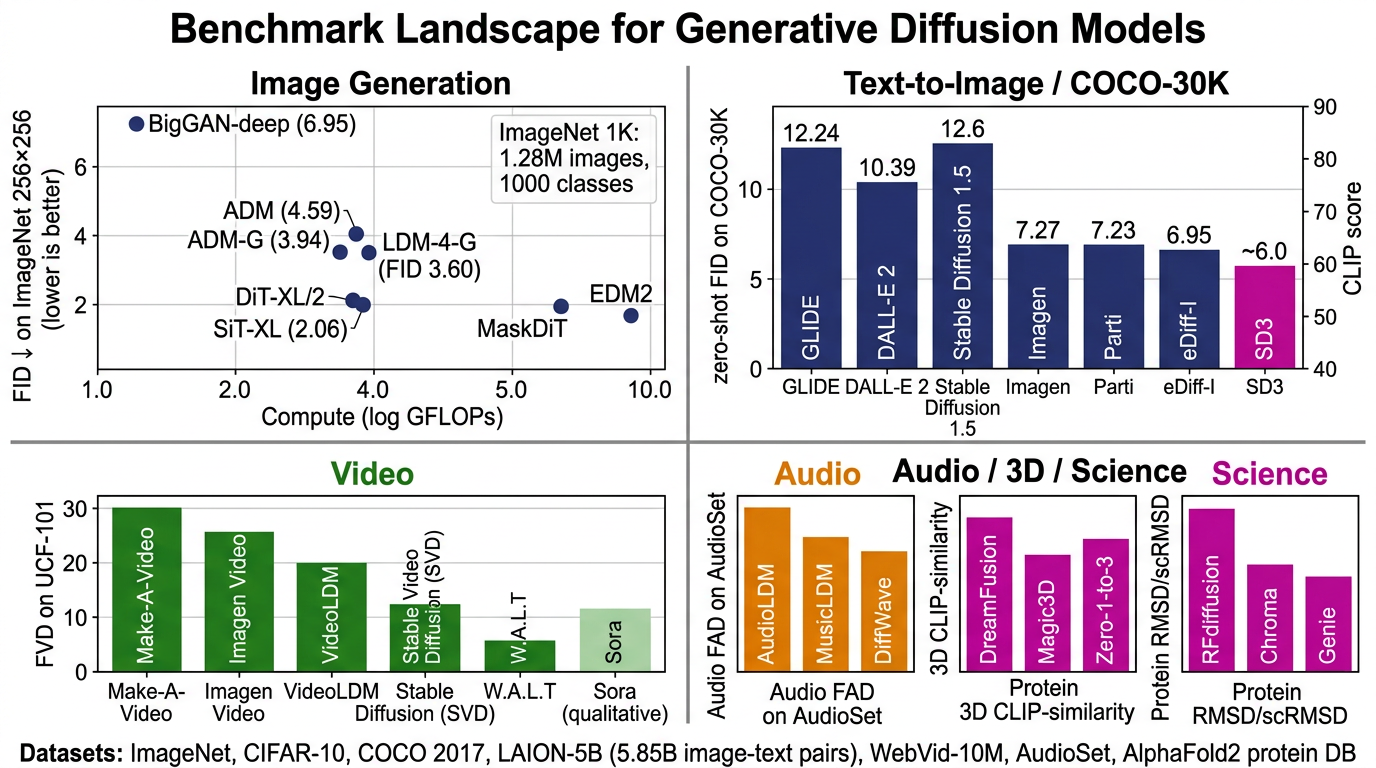
\includegraphics[keepaspectratio,alt={Benchmark landscape across image, video, audio, 3D, and protein evaluation regimes for generative diffusion models.}]{./figures/Generative-Diffusion-Models__fig4_benchmark_landscape.png}}
\caption{Benchmark landscape across image, video, audio, 3D, and protein evaluation regimes for generative diffusion models.}
\end{figure}

This section catalogues the datasets and metrics on which all flagship results are anchored, organized as image datasets, T2I benchmarks, video and audio benchmarks, metrics, compute costs, reproducibility, and a metrics summary table. Image datasets include CIFAR-10 (2009, 50K @ 32²), ImageNet-1K (2009, 1.28M / 1000 classes), CelebA-HQ (2017, 30K @ 1024²), FFHQ (2019, 70K @ 1024²), LSUN (2015, \textasciitilde3M per category), and MS COCO (2014, 118K with captions). Web-scraped corpora include LAION-400M / LAION-5B (2022, 5.85B image-text pairs) and CC12M (2021, 12M pairs). Video resources include WebVid-10M (2021, 10.7M video-caption pairs), HD-VILA-100M (2022, 100M HD clips), Panda-70M (2024, 70M curated clips), Kinetics-400/600/700 (2017, up to 700K clips), and UCF-101 (2012, 13K clips). Audio resources include AudioSet (2017, 2M+ clips), LJSpeech (2017, 24h speech), and MusicCaps (2023, 5.5K music captions). Other modalities draw on Objaverse / Objaverse-XL (2023, 800K / 10M 3D assets), HumanML3D (2022, \textasciitilde14K motion sequences), the PDB (\textasciitilde220K structures), and QM9 / GEOM-DRUGS (130K--2M molecules). Benchmarks include COCO-30K FID, DrawBench (200 prompts), PartiPrompts (1,632 prompts), T2I-CompBench, GenEval, HEIM, VBench, and EvalCrafter.

Diffusion advanced rapidly because the field converged early on a small set of canonical benchmarks and metrics that enabled apples-to-apples comparison. The training and evaluation corpora are concrete: CIFAR-10 (50K @ 32², FID \textless{} 2 is the modern target --- DDPM 3.17, EDM 1.79, EDM2 \textless{} 1.8), ImageNet-1K (1.28M / 1000 classes evaluated at 64²/128²/256²/512² --- anchors ADM 4.59, ADM-G 3.94, LDM-4-G 3.60, DiT-XL/2 2.27, EDM2-512 1.81, SiT-XL 2.06), CelebA-HQ (30K @ 1024²), FFHQ (70K @ 1024² for SR3 super-resolution), LSUN (\textasciitilde3M per category), MS COCO (118K + captions, 30K random prompts → COCO-30K FID), LAION-5B (5.85 billion image--text pairs, partially withdrawn pending CSAM remediation), CC12M, Objaverse-XL (10M 3D assets), HumanML3D motion (\textasciitilde14K sequences), the PDB (\textasciitilde220K protein structures), and QM9 / GEOM-DRUGS for molecules. Standard image metrics include FID (Heusel et al.~2017; biased toward InceptionV3 ImageNet distribution), CLIP-Score (Hessel et al.~2021; biased toward CLIP's training distribution), Precision/Recall (Kynkäänniemi et al.~2019; separates fidelity from diversity), LPIPS, KID, Vendi (diversity), and learned-reward HPS / ImageReward / PickScore. Video uses FVD (I3D features) and the 16-dimension VBench. Audio uses FAD (VGGish). Protein uses scRMSD against AlphaFold predictions of the designed sequence. Each metric has a documented bias (§11.6) and reporting multiple complementary metrics is now standard.

\subsection{Image datasets}\label{image-datasets}

The most-used image datasets for diffusion training and evaluation:

\begin{itemize}
\tightlist
\item
  \textbf{CIFAR-10} (Krizhevsky 2009): 50,000 training images of 32×32 resolution across 10 classes. Standard benchmark for unconditional image generation; FID under 2 is the modern target. DDPM 3.17, EDM 1.79, EDM2 \textless{} 1.8.
\item
  \textbf{ImageNet 1K} (Deng et al.~2009): 1.28 million training images, 1000 classes, evaluated at 64×64, 128×128, 256×256, 512×512. The dominant class-conditional benchmark. Anchors: ADM 256 FID 4.59, ADM-G 3.94, LDM-4-G 3.60, DiT-XL/2 2.27, EDM2 1.81 (512), SiT-XL 2.06.
\item
  \textbf{CelebA / CelebA-HQ} (Liu et al.~ICCV 2015): 200K celebrity images / 30K HQ at 1024×1024. Standard face-generation benchmark.
\item
  \textbf{FFHQ} (Karras et al.~CVPR 2019): 70,000 1024×1024 high-quality faces. SR3 reports 4× super-resolution PSNR/LPIPS on FFHQ.
\item
  \textbf{LSUN} (Yu et al.~2015): scenes including LSUN-Bedroom, LSUN-Cat, LSUN-Church (\textasciitilde3M images each at 256×256). ADM, DDPM, and LDM all report LSUN FID.
\item
  \textbf{MS COCO 2014/2017} (Lin et al.~ECCV 2014): 118K training images with five captions each. The default zero-shot text-to-image FID benchmark uses 30,000 random prompts (``COCO-30K FID''). Imagen 7.27, DALL-E 2 10.39, Parti 7.23, Stable Diffusion 1.5 ≈ 12.6.
\item
  \textbf{LAION-400M / LAION-5B} (Schuhmann et al.~2022): 5.85 billion image--text pairs scraped from Common Crawl, with quality and aesthetic subsets (LAION-aesthetics-v2-5+). Stable Diffusion was trained on a curated subset; LAION-5B remains the largest public T2I corpus. It has been a flashpoint for copyright concerns, and as of 2024 the dataset is partially withdrawn pending CSAM remediation.
\item
  \textbf{CC3M / CC12M} (Conceptual Captions): smaller cleanly-licensed image--text pairs.
\item
  \textbf{Visual Genome}, \textbf{OpenImages}, \textbf{WebLI} (Google internal), \textbf{DataComp}: alternative T2I corpora used by various systems.
\item
  \textbf{Objaverse / Objaverse-XL} (Deitke et al.~2023): 800K / 10M 3D assets used by Zero-1-to-3 and CLAY.
\end{itemize}

\subsection{Text-to-image benchmarks}\label{text-to-image-benchmarks}

Beyond COCO-30K FID, the community has built more demanding benchmarks:

\begin{itemize}
\tightlist
\item
  \textbf{DrawBench} (Saharia et al.~2022): 200 challenging prompts spanning compositionality, numbers, conflicting objects, and rare concepts. Used in human-preference studies for Imagen.
\item
  \textbf{PartiPrompts (P2)} (Yu et al.~2022): 1,632 prompts across 11 categories and 4 challenge dimensions.
\item
  \textbf{T2I-CompBench} (Huang et al.~2023): targeted compositional binding (color, shape, texture), spatial relations, non-spatial relations, and numeracy. SD3 leads as of 2024.
\item
  \textbf{GenEval} (Ghosh et al.~2024): automatic evaluator using object detectors to verify object presence, count, color, and spatial relations.
\item
  \textbf{HEIM} (Lee et al.~2023): holistic evaluation across 12 aspects (alignment, quality, originality, reasoning, knowledge, bias, toxicity, fairness, robustness, multilinguality, watermarking, efficiency).
\item
  \textbf{DALL-Eval} (Cho et al.~2022): structural and reasoning-driven assessment of T2I systems.
\end{itemize}

\subsection{Video and audio benchmarks}\label{video-and-audio-benchmarks}

Video:

\begin{itemize}
\tightlist
\item
  \textbf{UCF-101} (Soomro et al.~2012): 13K clips, 101 action classes. Standard FVD benchmark.
\item
  \textbf{Kinetics-400/600/700} (Carreira et al.~2017): up to 700K trimmed video clips. Imagen Video reports Kinetics-600 FVD.
\item
  \textbf{WebVid-10M} (Bain et al.~2021): 10.7M video--caption pairs at low resolution. Used for early text-to-video training.
\item
  \textbf{HD-VILA-100M} (Xue et al.~2022): 100M HD clips with captions.
\item
  \textbf{Panda-70M, OpenVid-1M, InternVid}: more recent curated T2V corpora.
\item
  \textbf{VBench} (Huang et al.~2024): comprehensive video-quality benchmark across 16 dimensions (subject consistency, background consistency, temporal flickering, motion smoothness, dynamic degree, aesthetic quality, imaging quality, etc.).
\item
  \textbf{EvalCrafter} (Liu et al.~2024): another holistic video-evaluation suite.
\end{itemize}

Audio:

\begin{itemize}
\tightlist
\item
  \textbf{LJSpeech} (Ito 2017): 13,100 LJ Speech utterances, \textasciitilde24 hours. Standard TTS benchmark for Grad-TTS, DiffWave.
\item
  \textbf{VCTK} (110 speakers, \textasciitilde44 h): multi-speaker TTS.
\item
  \textbf{AudioSet} (Gemmeke et al.~2017): 2M+ 10-second YouTube audio clips with sound-event labels. AudioLDM achieves FAD 1.97 on AudioSet evaluation.
\item
  \textbf{MusicCaps} (Agostinelli et al.~2023): 5,521 ten-second music clips with text captions, used by Noise2Music and MusicLDM.
\item
  \textbf{MTG-Jamendo, FMA}: music corpora.
\end{itemize}

\subsection{Metrics}\label{metrics}

The dominant metrics:

\begin{itemize}
\tightlist
\item
  \textbf{Fréchet Inception Distance (FID, Heusel et al.~NeurIPS 2017)}: Wasserstein-2 distance between Gaussian fits in InceptionV3 feature space; lower is better. Standard for image, with sFID and FID-CLIP variants (Jayasumana et al.~2024).
\item
  \textbf{Inception Score (IS, Salimans et al.~2016)}: KL divergence between conditional and marginal class distributions; higher is better. Largely deprecated for diffusion (Barratt \& Sharma 2018).
\item
  \textbf{Precision and Recall} (Kynkäänniemi et al.~NeurIPS 2019): nearest-neighbor coverage in feature space; separates fidelity from diversity.
\item
  \textbf{CLIP Score} (Hessel et al.~EMNLP 2021): cosine similarity between CLIP image and text embeddings; standard for T2I alignment.
\item
  \textbf{LPIPS} (Zhang et al.~CVPR 2018): perceptual similarity from a learned VGG/AlexNet backbone; used for restoration / super-resolution.
\item
  \textbf{PSNR / SSIM}: classical pixel and structural fidelity, still common in super-resolution and medical imaging.
\item
  \textbf{FVD} (Fréchet Video Distance, Unterthiner et al.~2018): video analogue of FID using I3D features.
\item
  \textbf{FAD} (Fréchet Audio Distance): audio analogue using VGGish features.
\item
  \textbf{KID} (Kernel Inception Distance, Bińkowski et al.~2018): unbiased alternative to FID.
\item
  \textbf{Vendi Score} (Friedman \& Dieng 2022): diversity metric based on the entropy of similarity-matrix eigenvalues.
\item
  \textbf{CLIP-IQA, GLIPS} (Aziz et al.~2024) and \textbf{GLIPS} for AI-generated photorealism assessment.
\item
  \textbf{HPS, ImageReward, PickScore}: human-preference reward models trained on millions of pairwise comparisons (used for RLHF-style fine-tuning of diffusion).
\item
  For video: VBench overall score, EvalCrafter scores, motion-quality metrics.
\item
  For protein: scRMSD (self-consistent RMSD against AlphaFold prediction of the designed sequence), TM-score, validity rate, novelty (vs PDB).
\end{itemize}

\subsection{Compute and cost benchmarks}\label{compute-and-cost-benchmarks}

{\def\LTcaptype{none} % do not increment counter
\begin{longtable}[]{@{}
  >{\raggedright\arraybackslash}p{(\linewidth - 6\tabcolsep) * \real{0.1679}}
  >{\raggedright\arraybackslash}p{(\linewidth - 6\tabcolsep) * \real{0.2443}}
  >{\raggedright\arraybackslash}p{(\linewidth - 6\tabcolsep) * \real{0.2901}}
  >{\raggedright\arraybackslash}p{(\linewidth - 6\tabcolsep) * \real{0.2977}}@{}}
\toprule\noalign{}
\begin{minipage}[b]{\linewidth}\raggedright
System
\end{minipage} & \begin{minipage}[b]{\linewidth}\raggedright
Backbone params
\end{minipage} & \begin{minipage}[b]{\linewidth}\raggedright
Training compute (GPU-hours)
\end{minipage} & \begin{minipage}[b]{\linewidth}\raggedright
Inference latency (50 NFE, 1024², A100)
\end{minipage} \\
\midrule\noalign{}
\endhead
\bottomrule\noalign{}
\endlastfoot
DDPM CIFAR-10 & 36M & \textasciitilde10K V100-h & n/a \\
ADM ImageNet 256 & 553M & \textasciitilde150K A100-h equivalent & \textasciitilde10s \\
Stable Diffusion 1.5 & 860M U-Net + 1B autoencoder/CLIP & \textasciitilde150K A100-h & \textasciitilde3.5s \\
SDXL & 2.6B U-Net + 700M text + 80M VAE & \textasciitilde700K A100-h & \textasciitilde7s \\
SD3 & up to 8B MMDiT + T5-XXL & tens of millions of A100-h (estimated) & \textasciitilde5s (28 NFE rectified) \\
DALL-E 3 & undisclosed & undisclosed & undisclosed \\
Imagen & 2B + 700M + 400M cascade & hundreds of thousands of TPU-h & \textasciitilde10s \\
Sora & several B (estimated) & tens of millions of GPU-h (estimated) & minutes per minute \\
Stable Video Diffusion & 1.5B & hundreds of thousands of A100-h & tens of seconds for 25 frames \\
RFdiffusion & \textasciitilde150M & hundreds of A100-days & seconds per backbone \\
Diffusion Policy & small (1D UNet) & dozens of GPU-h & sub-second per action \\
\end{longtable}
}

\subsection{Benchmark gaming and reproducibility concerns}\label{benchmark-gaming-and-reproducibility-concerns}

FID depends on InceptionV3 features trained on ImageNet, biasing evaluations toward natural-photograph styles (Jayasumana 2024 propose CMMD; Chong \& Forsyth 2019 document estimator bias). CLIP score favors prompts matching CLIP's training distribution. Human-preference rewards (HPS, ImageReward, MJ Bench) often track aesthetics over prompt fidelity. The community now reports multiple complementary metrics to triangulate quality.

\subsection{Reproducibility and tooling}\label{reproducibility-and-tooling}

Training reproducibility is uneven. SD 1.x scripts are public via \texttt{diffusers}. SDXL and SD3 weights are released but training data is partially undisclosed. Closed systems (DALL-E 3, Imagen, Sora, Midjourney) publish only blog reports. Standard tools include Hugging Face \texttt{diffusers} (\textgreater1M monthly downloads in 2025), \texttt{\$kohya\_s\$s} for LoRAs, and \texttt{ComfyUI} / \texttt{InvokeAI} for workflow construction.

\subsection{Dataset and benchmark summary table}\label{dataset-and-benchmark-summary-table}

{\def\LTcaptype{none} % do not increment counter
\begin{longtable}[]{@{}
  >{\raggedright\arraybackslash}p{(\linewidth - 6\tabcolsep) * \real{0.3191}}
  >{\raggedright\arraybackslash}p{(\linewidth - 6\tabcolsep) * \real{0.2128}}
  >{\raggedright\arraybackslash}p{(\linewidth - 6\tabcolsep) * \real{0.1383}}
  >{\raggedright\arraybackslash}p{(\linewidth - 6\tabcolsep) * \real{0.3298}}@{}}
\toprule\noalign{}
\begin{minipage}[b]{\linewidth}\raggedright
Dataset
\end{minipage} & \begin{minipage}[b]{\linewidth}\raggedright
Size
\end{minipage} & \begin{minipage}[b]{\linewidth}\raggedright
Modality
\end{minipage} & \begin{minipage}[b]{\linewidth}\raggedright
Use
\end{minipage} \\
\midrule\noalign{}
\endhead
\bottomrule\noalign{}
\endlastfoot
CIFAR-10 & 50K & image 32² & unconditional benchmark \\
ImageNet 1K & 1.28M / 1000 classes & image & class-conditional benchmark \\
CelebA-HQ & 30K & face 1024² & unconditional / personalization \\
FFHQ & 70K & face 1024² & super-res / face generation \\
LSUN & 3M+ per category & scene 256² & unconditional \\
COCO 2017 & 118K + captions & image & T2I FID-30K \\
LAION-400M / 5B & 400M / 5.85B & image+text & T2I training \\
CC12M & 12M & image+text & T2I training \\
WebVid-10M & 10.7M & video & T2V training \\
HD-VILA-100M & 100M & video & T2V training \\
Kinetics-600 & \textasciitilde480K & video & FVD benchmark \\
UCF-101 & 13K / 101 classes & video & unconditional video \\
AudioSet & 2M & audio & audio benchmark \\
LJSpeech & 13.1K / 24h & speech & TTS benchmark \\
MusicCaps & 5.5K & music+caption & music T2A \\
Objaverse-XL & 10M & 3D mesh & 3D generation \\
HumanML3D & 14K motion sequences & motion & motion generation \\
PDB & \textasciitilde220K structures & protein & protein design \\
MoleculeNet / QM9 / GEOM-DRUGS & 130K--2M & molecule & molecular generation \\
\end{longtable}
}

\subsection{Metrics summary table}\label{metrics-summary-table}

{\def\LTcaptype{none} % do not increment counter
\begin{longtable}[]{@{}
  >{\raggedright\arraybackslash}p{(\linewidth - 10\tabcolsep) * \real{0.1871}}
  >{\raggedright\arraybackslash}p{(\linewidth - 10\tabcolsep) * \real{0.0903}}
  >{\raggedright\arraybackslash}p{(\linewidth - 10\tabcolsep) * \real{0.0903}}
  >{\raggedright\arraybackslash}p{(\linewidth - 10\tabcolsep) * \real{0.1484}}
  >{\raggedright\arraybackslash}p{(\linewidth - 10\tabcolsep) * \real{0.2323}}
  >{\raggedright\arraybackslash}p{(\linewidth - 10\tabcolsep) * \real{0.2516}}@{}}
\toprule\noalign{}
\begin{minipage}[b]{\linewidth}\raggedright
Metric
\end{minipage} & \begin{minipage}[b]{\linewidth}\raggedright
Modality
\end{minipage} & \begin{minipage}[b]{\linewidth}\raggedright
Range
\end{minipage} & \begin{minipage}[b]{\linewidth}\raggedright
Direction
\end{minipage} & \begin{minipage}[b]{\linewidth}\raggedright
Strength
\end{minipage} & \begin{minipage}[b]{\linewidth}\raggedright
Weakness
\end{minipage} \\
\midrule\noalign{}
\endhead
\bottomrule\noalign{}
\endlastfoot
FID & image & ≥0 & lower better & standard, well-correlated with human & InceptionV3 bias \\
IS & image & ≥1 & higher better & simple & doesn't measure diversity well \\
Precision / Recall & image & {[}0,1{]} & higher better & separates fidelity \& diversity & feature-space dependent \\
CLIP score & T2I & {[}-1,1{]} & higher better & measures alignment & favors CLIP's prior \\
LPIPS & image pair & {[}0,∞) & lower better & perceptual & requires reference \\
PSNR / SSIM & image pair & dB / {[}0,1{]} & higher better & classical & not perceptual \\
FVD & video & ≥0 & lower better & video analogue of FID & small-sample noise \\
FAD & audio & ≥0 & lower better & audio analogue & VGGish biased \\
KID & image & ≥0 & lower better & unbiased & smaller signal than FID \\
Vendi & any & ≥1 & higher better diversity & diversity-only & needs similarity kernel \\
HPS / ImageReward / PickScore & T2I & learned reward & higher better & trained on humans & favors aesthetic, not literal alignment \\
CMMD (Jayasumana 2024) & image & ≥0 & lower better & unbiased CLIP-based & new, not yet universal \\
scRMSD & protein design & Å & lower better & functional validity & requires AlphaFold pass \\
\end{longtable}
}

This benchmark and metric infrastructure is what enables the rapid pace of progress: a new method is meaningful only if it improves at least one standard score, ideally without degrading others. Section 12 turns to the failure modes that these metrics routinely miss --- memorization, compositional binding, bias, safety bypass, and physical implausibility --- which together define the deployment envelope.

\section{Limitations, Failure Modes, and Open Problems}\label{limitations-failure-modes-and-open-problems}

This section catalogs the failure modes that the metrics of §11 routinely miss, organized as memorization and copyright, compositional and reasoning failures, bias and safety, compute and access, modality-specific limitations, and theoretical gaps.

Diffusion's dominance comes with a well-documented catalog of failure modes. The technical category includes compositional binding (``a red ball and a blue cube'' yields color-mixed objects), numeracy (``five apples'' → 3--7), spatial relations (``left of'' / ``above''), text rendering (SD 1.5 fails \textasciitilde50\% of simple words; SDXL is improved; SD3 with T5-XXL and MMDiT is markedly better but imperfect), and reasoning involving negation. The statistical category includes verbatim memorization (Carlini et al., USENIX Security 2023, extracted \textasciitilde109 LAION images from Stable Diffusion 1.4 across 175M sampling attempts) and near-copy replication (Somepalli et al., CVPR 2023, \textasciitilde1.88\% of SD outputs are detectable copies). The societal category includes deepfake misuse, NSFW safety-filter bypasses (Rando et al.~2022 showed SD's CLIP-embedding filter is paraphrasable), copyright (Getty Images v. Stability AI; Andersen v. Stability/Midjourney/DeviantArt; NYT v. OpenAI; all unresolved as of 2026), energy footprint (\textasciitilde30 MWh per SD 1.5 training run, \textasciitilde10 t CO₂; tens of millions of GPU-hours for Sora), and access asymmetry concentrated in OpenAI, Google, Stability AI, Black Forest Labs, Tencent, and Baidu. The epistemic category includes the missing theoretical account of why CFG at large w (5--10) helps, the score-mismatch at low noise levels, and the lack of LLM-style influence functions for diffusion. Each subsection documents one category with citations, mitigations (deduplication, concept erasure, FairDiffusion, Stable Signature watermarks, dynamic thresholding), and residual risk.

\subsection{Memorization, copyright, and replication}\label{memorization-copyright-and-replication}

Carlini, Hayes, Nasr, Jagielski, Sehwag, Tramèr, Balle, Ippolito, and Wallace's \emph{Extracting Training Data from Diffusion Models} (USENIX Security 2023) demonstrated that Stable Diffusion 1.4 can be made to verbatim reproduce \textasciitilde109 specific training images out of 175 million sampling attempts using carefully crafted prompts. Somepalli, Singla, Goldblum, Geiping, and Goldstein's \emph{Diffusion Art or Digital Forgery?} (CVPR 2023) showed that approximately 1.88\% of Stable Diffusion outputs are detectable copies of training images. Both works tied memorization to (a) data deduplication failures (LAION's 5B raw set has many near-duplicates), (b) heavily-captioned images appearing repeatedly, and (c) high CFG values that push outputs toward exact training matches.

The implication for practice: any diffusion model trained on web-scraped data should be assumed to memorize a non-trivial slice of its training set, with implications for copyright (Getty Images v. Stability AI, ongoing), privacy (medical or face images), and provenance. Mitigations include training-set deduplication (used by Imagen and Pixart-α), caption diversity, lower CFG, and post-training ``concept erasure'' (Wu et al.~2024; Gandikota et al.~2023). The \emph{Stable Signature} (Fernandez et al.~ICCV 2023) embeds robust watermarks in the autoencoder so that diffusion outputs carry a hidden owner signature.

\subsection{Compositional binding, text rendering, and reasoning failures}\label{compositional-binding-text-rendering-and-reasoning-failures}

T2I models notoriously fail on (a) compositional binding (the prompt ``a red ball and a blue cube'' often produces a blue ball or color-mixed objects), (b) numeracy (asking for ``five apples'' reliably produces 3--7), (c) spatial relations (the prompt ``left of'' / ``above'' is unreliable), (d) text rendering (legible text in the generated image is challenging --- SD 1.5 fails \textasciitilde50\% of the time on simple words; SDXL is improved; SD3 with T5-XXL and MMDiT is markedly better but still imperfect), and (e) reasoning (the prompt ``a table with seven items, none red'' requires negation that CFG cannot directly provide).

T2I-CompBench specifically targets these failures and has quantitative ratings for each subset; SD3 and Flux-pro lead as of 2024 but human studies show all systems retain a substantial gap from prompt fidelity. \emph{RPG} (Yang et al.~2024), \emph{MIGC}, \emph{Attend-and-Excite} (Chefer et al.~2023), and \emph{Diffusion-RPG} are mitigations that re-route attention or perform per-region generation; they help but do not fully solve compositional binding.

Hand and finger anatomy is a famous T2I failure: generated humans frequently have 6 or 4 fingers, twisted wrists, or floating limbs. SDXL substantially mitigates this via training on better-curated human imagery; SD3 mitigates further; specialized add-ons (e.g., Hand Refiner with ControlNet on hand poses) provide nearly photographic hands.

\subsection{Bias, fairness, and safety filters}\label{bias-fairness-and-safety-filters}

Diffusion models inherit biases of their training data. Studies have shown that SD 1.5 prompted with ``CEO'' returns predominantly male images; ``nurse'' returns predominantly female; ``criminal'' exhibits racial skew (Naik \& Nushi 2023; Bianchi et al.~2023 FAccT). \emph{FairDiffusion} (Luo et al.~Science Advances 2025) introduces fair Bayesian perturbation to mitigate demographic bias in latent diffusion specifically for medical imaging; analogous bias-mitigation work exists for T2I.

Safety filters are imperfect. Rando, Paleka, Lindner, Heim, and Tramèr's \emph{Red-Teaming the Stable Diffusion Safety Filter} (2022) showed that the official SD safety filter, which compares CLIP image embeddings to known unsafe concepts, can be bypassed by simple paraphrases or adversarial prompts. Subsequent work has shown that even filtered models can produce NSFW content via concept-erasure-resistant prompts. The detection side has \emph{DIRE} (Wang et al.~ICCV 2023) for distinguishing diffusion-generated images via reconstruction error, \emph{DE-FAKE} (Sha et al.~2023) for fake-image attribution, and the \emph{Stable Signature} watermark.

\subsection{Compute, environmental cost, and access inequality}\label{compute-environmental-cost-and-access-inequality}

Training Stable Diffusion 1.5 reportedly consumed \textasciitilde150K A100-GPU-hours, roughly 30 MWh and \textasciitilde10 metric tons of CO₂ at typical grid intensities. SDXL and SD3 scale this several-fold; Sora is reported to consume tens of millions of GPU-hours. The economic footprint is concentrated in companies with the GPU access to train at this scale (OpenAI, Google, Stability AI, Tencent, Baidu, Black Forest Labs / Flux), creating an access asymmetry. Reproducibility for academic groups is gated by compute, although Pixart-α (1/10 SDXL compute) and PixArt-Σ have shown that careful curriculum design partially closes the gap.

Inference cost is also non-trivial: a single SDXL image at 1024² consumes \textasciitilde70--100 J on A100. Globally, image generation at billion-image-per-month volumes is now an industrial-grade energy load.

\subsection{Modality-specific limitations}\label{modality-specific-limitations}

For video, the most prominent limitation is \emph{temporal coherence over long horizons}: even Sora exhibits gradual identity drift over 30+ seconds, and physical inconsistencies (objects vanishing, fluids violating mass conservation, pedestrians vanishing into walls) are documented in OpenAI's own technical report. \emph{Camera control}, \emph{physical accuracy}, and \emph{long-horizon causality} remain open.

For audio, \emph{long-form coherence} (multi-minute music with consistent motifs) is harder than 30-second clip generation. \emph{Lyrics-aligned} music generation lags behind instrumental.

For 3D, \emph{multi-view inconsistency} (the ``Janus problem'' where a generated 3D object has two front faces) plagues SDS-based methods; multi-view diffusion (MVDream, SyncDreamer, Zero-1-to-3++) helps. \emph{Watertight, manufacturable mesh generation} remains a 2024--2026 open problem.

For protein, \emph{all-atom co-design with ligands} and \emph{evolutionary plausibility} (designs are sometimes structurally valid but biologically uncommon) are active fronts.

For robotics, \emph{out-of-distribution generalization} and \emph{real-time inference} are persistent. Consistency Policy addresses inference latency but distribution shift remains.

\subsection{Theoretical and methodological gaps}\label{theoretical-and-methodological-gaps}

Despite empirical progress, several theoretical questions remain open. (a) Why classifier-free guidance works at large w (5--10) is not fully understood; recent analyses (Karras et al.~2024 EDM2, others) suggest CFG implicitly samples from a tilted distribution but the optimal w is ad hoc. (b) The \emph{score-mismatch} between the trained ε\emph{θ and the true score during sampling --- particularly at small noise levels --- produces measurable but unaddressed sample-quality losses (Choi et al.~2022). (c) The }equivalence and gap* between rectified flow, EDM, and classical score matching at sufficient compute scale is still being mapped empirically. (d) \emph{Generalization vs.~memorization} at the level of individual training points is not well-characterized; we lack tools analogous to LLM influence functions for diffusion. (e) \emph{Sampling robustness} under model errors --- what happens when ε*θ has bounded prediction error --- is studied (Lee et al.~2022 convergence) but practical guarantees are weak.

\subsection{Failure-mode summary}\label{failure-mode-summary}

{\def\LTcaptype{none} % do not increment counter
\begin{longtable}[]{@{}
  >{\raggedright\arraybackslash}p{(\linewidth - 6\tabcolsep) * \real{0.1884}}
  >{\raggedright\arraybackslash}p{(\linewidth - 6\tabcolsep) * \real{0.4348}}
  >{\raggedright\arraybackslash}p{(\linewidth - 6\tabcolsep) * \real{0.3116}}
  >{\raggedright\arraybackslash}p{(\linewidth - 6\tabcolsep) * \real{0.0652}}@{}}
\toprule\noalign{}
\begin{minipage}[b]{\linewidth}\raggedright
Failure
\end{minipage} & \begin{minipage}[b]{\linewidth}\raggedright
Example
\end{minipage} & \begin{minipage}[b]{\linewidth}\raggedright
Mitigation
\end{minipage} & \begin{minipage}[b]{\linewidth}\raggedright
Residual
\end{minipage} \\
\midrule\noalign{}
\endhead
\bottomrule\noalign{}
\endlastfoot
Verbatim memorization & Stable Diffusion reproduces \textasciitilde109 LAION images (Carlini 2023) & dedup, lower CFG, concept erasure & non-zero \\
Near-copy replication & \textasciitilde1.88\% of SD outputs copy training (Somepalli 2023) & curated training & residual \\
Compositional binding & wrong color/object pairing & Attend-and-Excite, RPG, SD3 & partial \\
Numeracy & ``5 apples'' gives 3--7 & object-detection re-prompting & partial \\
Text rendering & unreadable letters & T5-XXL + MMDiT & improving \\
Hand anatomy & 6 fingers / mangled wrists & curated data, ControlNet pose & improving \\
Bias (gender/race) & profession-stereotyped outputs & balanced data, FairDiffusion & open \\
NSFW evasion & safety filter bypass via adversarial prompt & red-teaming, post-hoc detector & partial \\
Deepfakes / misinformation & generated political images & watermark (Stable Signature), DIRE detector & open \\
Copyright lawsuits & Getty v. Stability AI & licensing, data provenance & open \\
Long-horizon video drift & Sora identity drift after 30+ s & longer-context attention & open \\
Multi-view ``Janus'' 3D & two front faces & multi-view diffusion & partial \\
Physics violations & impossible fluid motion & physics-aware loss & open \\
Energy footprint & \textasciitilde30 MWh per SD 1.5 training & efficient training, distillation & partial \\
Access inequality & only large labs train foundation models & open weights / Pixart efficiency & partial \\
Reasoning / negation & ``no red'' fails & constrained decoding & open \\
\end{longtable}
}

\subsection{Adversarial and security failures}\label{adversarial-and-security-failures}

Diffusion as inverse-problem prior is more robust than direct networks (Wang 2023). As generators, diffusion is attackable: Glaze and Nightshade poison training data; PhotoGuard immunizes images from editors. Membership inference attacks have been demonstrated (Carlini 2023; Hu 2024). DP-DDPM (Dockhorn 2023) trades a small FID hit for ε-DP guarantees.

\subsection{Open problems summary}\label{open-problems-summary}

{\def\LTcaptype{none} % do not increment counter
\begin{longtable}[]{@{}
  >{\raggedright\arraybackslash}p{(\linewidth - 2\tabcolsep) * \real{0.5000}}
  >{\raggedright\arraybackslash}p{(\linewidth - 2\tabcolsep) * \real{0.5000}}@{}}
\toprule\noalign{}
\begin{minipage}[b]{\linewidth}\raggedright
Open problem
\end{minipage} & \begin{minipage}[b]{\linewidth}\raggedright
Status as of 2026
\end{minipage} \\
\midrule\noalign{}
\endhead
\bottomrule\noalign{}
\endlastfoot
One-step matching of multi-step quality & partially solved; \textasciitilde10\% gap on prompt comprehension \\
Long-form video coherence (5+ min) & Sora demonstrates 60s; longer is open \\
All-atom protein co-design with ligands & Boltz-1 / RoseTTAFold AA + diffusion in progress \\
Real-time interactive video at 1080p & feasible at 24 fps with distillation, near term \\
Theoretical foundations of CFG & empirical insights; no clean theory \\
Compositional binding at \textgreater5 objects & active; SD3 / SD-Eclipse improving \\
Memorization auditing tooling & nascent; analogous to LLM extraction \\
Diffusion-RLHF alignment & DPO-Diffusion, Diffusion-DPO, ImageReward; active \\
Standardized scientific generative benchmarks & sparse; T2I-CompBench-for-proteins not yet exists \\
Fair distributional generation & FairDiffusion, BiasPainter; open in general \\
Efficient long-context video diffusion (Mamba/SSM) & early prototypes \\
Provenance and watermarking standards & C2PA, Stable Signature; partial adoption \\
Multimodal any-to-any foundation diffusion & CoDi, Versatile Diffusion; not at LLM scale \\
\end{longtable}
}

\subsection{Why these limitations matter}\label{why-these-limitations-matter}

Failure modes shape deployment risk. The Getty v. Stability AI lawsuit, the EU AI Act, the 2024 mandatory-watermarking requirements, U.S. Executive Order 14110, and NIST's adversarial-ML report (Vassilev 2024) all target the modes above. As diffusion moves from research to infrastructure, these limitations determine which applications are deployable. Section 13 calibrates predictions against which limitations are most likely to resolve.

\section{Future Directions and Predictions}\label{future-directions-and-predictions}

This section names the trajectories most likely to resolve the open problems of §12, organized as one-step generators, multimodal foundations, scientific co-design, theoretical unification, post-training alignment, safety and provenance, on-device sampling, and three falsifiable headline forecasts.

Progress since 2020 has consistently outpaced the field's own forecasts, so our prediction discipline must be both ambitious and falsifiable. We outline four trajectories with concrete forecasts checkable against the empirical record by 2027--2030. The first is \emph{one-step foundation generators} --- closing the residual quality gap (FID within \textasciitilde10\%, CLIP-Score within 5--10 points) between distilled students (LCM, SDXL-Turbo, Hyper-SD, Lightning, MAR) and multi-step teachers, with rectified-flow training as the default. The second is \emph{multimodal any-to-any diffusion} --- a single 20--50B-parameter MMDiT-style backbone whose tokens span text, image patches, audio frames, video patches, motion, and 3D, generalizing Versatile Diffusion, CoDi, and NExT-GPT. The third is \emph{scientific co-design and embodied diffusion} --- all-atom protein design integrating Boltz-1 and AlphaFold-3, closed-loop wet-lab platforms (Latent-Y, Generate Biomedicines, Iambic, Inceptive, Cradle), GenCast-style climate ensembles, MatterGen / DiffCSP for crystal-structure generation, and Consistency Policy for real-time robotics. The fourth is \emph{theoretical unification} --- flow matching, rectified flow, score SDE, EDM preconditioning, and Schrödinger bridges consolidated into a single textbook chapter on flow-based generative modeling on time-indexed paths. We commit to three falsifiable headline forecasts in §13.9 (one-step T2I quality, 5-minute video coherence, FDA/EMA-approved diffusion-designed therapeutic) and explicitly disclaim what we are \emph{not} predicting in §13.10.

\subsection{Toward one-step foundation generators}\label{toward-one-step-foundation-generators}

The clearest near-term direction is closing the residual quality gap between distilled one-step generators and multi-step teachers. As of late 2024, SDXL-Turbo, LCM, Hyper-SD, and Lightning match teachers within \textasciitilde10\% on FID and 5--10 points on CLIP-Score / GenEval. The gap concentrates in compositional binding under high CFG, small-font text rendering, and low-frequency layout decisions. Likely closing approaches include rectified-flow training as default (SD3, Flux), stronger adversarial distillation (StyleGAN-T successors), multi-teacher score distillation, and block-causal MMDiT masking. We forecast that by 2027 the leading open one-step generator will reach COCO-30K FID \textless{} 7 and CLIP-Score \textgreater{} 0.32 at sub-200 ms latency on consumer GPUs.

MAR-style autoregressive-meets-diffusion (Li 2024) achieves FID 1.55 on ImageNet 256 by interleaving AR token order with per-token diffusion. We expect this to dominate foundation models that must jointly generate and condition on long contexts.

\subsection{Multimodal and any-to-any diffusion}\label{multimodal-and-any-to-any-diffusion}

SD3's MMDiT showed text and image tokens can share attention. Versatile Diffusion (2023), CoDi (2023), and NExT-GPT extend to text + image + audio + video. The next step is foundation any-to-any diffusion: one backbone whose tokens span text, image patches, audio frames, video patches, motion, and 3D. Obstacles are tokenization parity, sub-quadratic attention for long sequences (Mamba/SSM helps), and multimodal data curation. By 2027 we expect a 20--50B-parameter multimodal flow-matching foundation model supporting text⇄image⇄video⇄audio at competitive benchmark scores. Cross-modality also has scientific applications: text-to-protein, text-to-molecule, structure-to-DNA (Wachi 2024).

\subsection{Scientific co-design and embodied diffusion}\label{scientific-co-design-and-embodied-diffusion}

By 2027 we expect: all-atom protein design integrating Boltz-1 and AlphaFold-3 with diffusion sampling; closed-loop wet-lab platforms (Latent-Y, Generate Biomedicines, Iambic, Inceptive) delivering clinical candidates; crystal-structure diffusion (MatterGen, DiffCSP) entering industrial use; and GenCast-style probabilistic weather forecasting at sub-kilometer resolution. In robotics, Diffusion Policy, Consistency Policy, and Diffuser / Decision Diffuser will be standard components, with 100+ Hz inference plausible. We forecast that by 2027 at least one FDA- or EMA-approved therapeutic antibody will have a diffusion-designed lead.

\subsection{Theoretical unification under flow matching and Schrödinger bridges}\label{theoretical-unification-under-flow-matching-and-schruxf6dinger-bridges}

Stochastic interpolants (Albergo 2023), flow matching (Lipman 2023), rectified flow (Liu 2023), Schrödinger bridges (De Bortoli 2021), and EDM preconditioning each give a partial unification. Remaining theoretical work covers NFE-vs-error bounds, optimal w(t) for CFG, the role of equivariance, and connections to optimal transport beyond the Schrödinger-bridge limit. By 2027--2028 the textbook view will be one chapter on flow-based generative modeling on time-indexed paths.

\subsection{Distribution alignment, reward fine-tuning, and post-training}\label{distribution-alignment-reward-fine-tuning-and-post-training}

LLM-style RLHF has diffusion analogues: Diffusion-DPO (Wallace 2024), DRaFT (Clark 2024), DDPO (Black 2024), and ImageReward / PickScore / HPS rewards. By 2026 post-training (DPO, RLHF, RLAIF) will be standard in diffusion, with ``base'' and ``preference-aligned'' pairs shipped together. Risks include preference-overfitting that erases prompt diversity.

\subsection{Safety, provenance, and regulation}\label{safety-provenance-and-regulation}

Watermarking will become mandatory under the EU AI Act, U.S. EO 14110, China's GenAI Service Management Provisions, and the C2PA standard. Stable Signature (Fernandez 2023) and successors will be deployed at scale. Detection (DIRE, DE-FAKE) will improve. Licensed-data foundation models (Adobe Firefly) will grow in enterprise share as Getty v. Stability, Andersen, and NYT v. OpenAI partially resolve.

\subsection{Sampling, hardware, and on-device diffusion}\label{sampling-hardware-and-on-device-diffusion}

Consumer-device diffusion is already real: Apple CoreML, Google MobileDiffusion, NVIDIA TensorRT, AMD ROCm. By 2027 on-device 1024² T2I will run in \textless500 ms on flagship phones. Specialized accelerators (Cerebras, Etched, Groq, Tenstorrent) will support diffusion-specific kernels.

\subsection{Open-problem table and falsifiable forecasts}\label{open-problem-table-and-falsifiable-forecasts}

{\def\LTcaptype{none} % do not increment counter
\begin{longtable}[]{@{}
  >{\raggedright\arraybackslash}p{(\linewidth - 6\tabcolsep) * \real{0.2500}}
  >{\raggedright\arraybackslash}p{(\linewidth - 6\tabcolsep) * \real{0.2016}}
  >{\raggedright\arraybackslash}p{(\linewidth - 6\tabcolsep) * \real{0.2339}}
  >{\raggedright\arraybackslash}p{(\linewidth - 6\tabcolsep) * \real{0.3145}}@{}}
\toprule\noalign{}
\begin{minipage}[b]{\linewidth}\raggedright
Open problem
\end{minipage} & \begin{minipage}[b]{\linewidth}\raggedright
2026 status
\end{minipage} & \begin{minipage}[b]{\linewidth}\raggedright
2027 forecast
\end{minipage} & \begin{minipage}[b]{\linewidth}\raggedright
2030 forecast
\end{minipage} \\
\midrule\noalign{}
\endhead
\bottomrule\noalign{}
\endlastfoot
One-step foundation T2I quality & within 10\% of teacher & matches teacher on FID + CLIP & exceeds teacher (preference-aligned) \\
Long-form video coherence & 60 s coherent (Sora) & 5-min coherent & feature-length on demand \\
Real-time interactive video & early demos & 720p / 24 fps consumer & 4K / 60 fps cloud \\
Multimodal any-to-any & bespoke (CoDi, Versatile) & shared MMDiT 20--50B & foundation multimodal at LLM scale \\
All-atom protein co-design & RFdiffusion + LigandMPNN & unified diffusion + ligand & clinical pipelines using unified models \\
Diffusion-RLHF alignment & nascent (DPO-Diffusion) & standard post-training & cf.~RLAIF / Constitutional AI \\
Watermarking ubiquity & partial (SS) & mandatory in EU/US & C2PA-compliant industry-wide \\
Theoretical unification & flow-matching dominant & textbook unified & mature theory \\
Memorization auditing & research-only & tooling shipped & regulatory audit standard \\
Open-source vs.~closed gap & small (Flux ≈ MJ) & possibly narrowing further & uncertain (compute frontier matters) \\
\end{longtable}
}

\subsection{Three falsifiable headline forecasts}\label{three-falsifiable-headline-forecasts}

We commit to three falsifiable predictions for benchmarking purposes:

\begin{enumerate}
\def\labelenumi{\arabic{enumi}.}
\tightlist
\item
  \textbf{Forecast A (sample efficiency).} By 31 December 2027, the leading open-weight T2I model will achieve COCO-30K zero-shot FID \textless{} 7 \emph{and} CLIP-Score \textgreater{} 0.32 in ≤ 4 NFE on consumer GPU, matching or exceeding 2023 SDXL multi-step quality at one-tenth the inference cost.
\item
  \textbf{Forecast B (video diffusion).} By 31 December 2027, an open-weight or commercially-available video diffusion system will produce coherent 5-minute 1080p videos with VBench overall score \textgreater{} 85 (currently SOTA is \textasciitilde80 for 5-second clips).
\item
  \textbf{Forecast C (scientific design).} By 31 December 2030, at least one FDA- or EMA-approved therapeutic biologic will have been substantially designed by a diffusion-based generative model in its discovery pipeline (i.e., the lead candidate's variable region or scaffold was generated by RFdiffusion / Chroma / Latent-Y or successor).
\end{enumerate}

These forecasts can be checked by examining the relevant benchmarks and the FDA / EMA approval databases.

\subsection{What we are not predicting}\label{what-we-are-not-predicting}

We avoid predictions about (a) displacement of diffusion by a new paradigm (no current evidence); (b) AGI from diffusion alone (diffusion is generation, not reasoning); (c) pixel-level indistinguishability across all niches; and (d) quantitative compute trajectories, since chip supply and datacenter buildout dominate.

\subsection{Closing perspective on future directions}\label{closing-perspective-on-future-directions}

Generative diffusion is converging toward unified flow-matching foundations, distilled few-step inference, shared multimodal token spaces, and scientific design platforms. The ``what comes next'' questions are now engineering and integration rather than open algorithmic mysteries. The 2025--2030 era will be defined by systemic integration into scientific discovery, creative tooling, robotics, and content provenance, while resolving the failure modes catalogued in §12.

\section{Conclusion and Glossary}\label{conclusion-and-glossary}

This survey has presented a comprehensive, retrieval-friendly account of generative diffusion models as of 2026: mathematical foundations (§2), historical trajectory (§3), five-axis taxonomy (§4), architectural building blocks (§5), training objectives (§6), sampling and acceleration (§7), conditioning and guidance (§8), modality-specific deployments (§9), scientific applications (§10), datasets and benchmarks (§11), failure modes (§12), and forecasts (§13). We close with a synthesis, a terminology glossary for quick reference, and pointers to open resources. Read end-to-end the document is a tutorial; consulted by section it is a keyword-searchable reference linking specific named systems (DDPM, ADM, LDM, SDXL, SD3, DiT, EDM, RFdiffusion, Diffusion Policy, AudioLDM, Sora) to specific empirical anchors (FID, CLIP-Score, FVD, FAD, scRMSD), datasets (CIFAR-10, ImageNet-1K, COCO, LAION-5B, Kinetics, AudioSet, PDB), and concrete failure modes.

\subsection{Synthesis}\label{synthesis}

Generative diffusion began as a 2015 nonequilibrium-thermodynamics framework (Sohl-Dickstein), dormant for half a decade, that became between 2020 and 2024 the dominant paradigm for high-fidelity controllable generation across imagery, video, audio, 3D assets, motion, proteins, molecules, medical images, and robot trajectories. Three intellectual moves powered the rise: DDPM's \(L_s\)imple (Ho 2020), score-SDE unification (Song 2021), and latent diffusion (Rombach 2022). Three engineering moves powered deployment: classifier-free guidance (Ho \& Salimans 2022), Diffusion Transformers (Peebles \& Xie 2023), and consistency-style distillation plus rectified flow (Song 2023; Liu 2023).

The current state is fluid engineering atop a stable theoretical base. SD3, Sora, RFdiffusion, Diffusion Policy, AudioLDM, Pixart-Σ, Flux, and Latent-Y are variants of one recipe: a Gaussian forward schedule, a learned U-Net or DiT reverse predictor, classifier-free or structural guidance, and a fast sampler. They differ in representation, scale, and corpus. Open challenges (memorization, compositional binding, long-form video, all-atom co-design, multimodal foundations, theoretical unification) are detailed in §12, §13, and §15.

\subsection{Terminology glossary}\label{terminology-glossary}

{\def\LTcaptype{none} % do not increment counter
\begin{longtable}[]{@{}
  >{\raggedright\arraybackslash}p{(\linewidth - 2\tabcolsep) * \real{0.3333}}
  >{\raggedright\arraybackslash}p{(\linewidth - 2\tabcolsep) * \real{0.6667}}@{}}
\toprule\noalign{}
\begin{minipage}[b]{\linewidth}\raggedright
Term
\end{minipage} & \begin{minipage}[b]{\linewidth}\raggedright
Definition
\end{minipage} \\
\midrule\noalign{}
\endhead
\bottomrule\noalign{}
\endlastfoot
Forward (noising) process & The Markov chain q(x\emph{t \textbar{} x}\{t−1\}) that adds Gaussian noise according to schedule β\_t. \\
Reverse (denoising) process & The learned chain p\emph{θ(x}\{t−1\} \textbar{} x\_t) that inverts the forward process. \\
Variance schedule β\_t & Per-step Gaussian noise variance; can be linear, cosine, EDM-σ. \\
ᾱ\_t & Cumulative product ∏\_s (1 − β\_s); determines how much of x\_0 remains at time t. \\
Score s\_θ(x, t) & Estimate of ∇\_x log p\_t(x); the gradient of the noisy log-density. \\
ε-prediction & Network outputs the injected noise ε. \\
x\_0-prediction & Network outputs the clean datum directly. \\
v-prediction & Network outputs v\_t = √ᾱ\_t ε − √(1−ᾱ\_t) x\_0; balanced parameterization. \\
Probability flow ODE & Deterministic ODE whose marginals match the SDE's. \\
Classifier guidance & Modifying the score with ∇log p(y\textbar x); requires noisy classifier. \\
Classifier-free guidance (CFG) & (1+w) ε\_cond − w ε\_uncond combination at inference. \\
DDIM & Deterministic non-Markovian sampler with arbitrary step count. \\
DPM-Solver & Closed-form high-order ODE sampler. \\
Heun integrator & Predictor-corrector second-order ODE method used by EDM. \\
Consistency model & f\_θ(x\_t,t)→x\_0 self-consistent across timesteps; supports 1-step generation. \\
Latent diffusion & Diffusion in the bottleneck of a pretrained autoencoder. \\
LDM & Latent Diffusion Model (Rombach 2022). \\
LAION-5B & 5.85B image-text pairs used for T2I training. \\
LoRA & Low-rank adaptation for personalization. \\
ControlNet & Hypernetwork for structural conditioning (edges/depth/pose/segmentation). \\
DreamBooth & Subject-personalization via full fine-tuning. \\
Textual Inversion & Subject-personalization via new token embedding. \\
FID & Fréchet Inception Distance; standard image-quality metric. \\
CLIP-Score & Cosine similarity in CLIP feature space; T2I alignment. \\
FVD & Fréchet Video Distance; video analogue of FID. \\
FAD & Fréchet Audio Distance; audio analogue. \\
LPIPS & Perceptual similarity from a learned VGG/AlexNet feature space. \\
Vendi Score & Diversity metric. \\
HPS / ImageReward / PickScore & Learned human-preference rewards. \\
DiT & Diffusion Transformer (Peebles \& Xie 2023). \\
MMDiT & Multimodal DiT used in Stable Diffusion 3. \\
Flow matching & Vector-field regression objective on data-noise interpolant. \\
Rectified flow & Iteratively re-flowed straight-line generative paths. \\
Stochastic interpolants & Unifying framework for flow + diffusion. \\
EDM & Elucidating the Design Space (Karras 2022); preconditioned diffusion. \\
Min-SNR weighting & Loss reweighting by min(γ, SNR(t)). \\
Score Distillation Sampling (SDS) & Loss for using 2D diffusion priors to optimize 3D models. \\
Diffusion Posterior Sampling (DPS) & Inverse-problem sampler combining diffusion prior with likelihood gradient. \\
RFdiffusion & Diffusion-based protein design (Watson 2023, Nature). \\
Chroma & Programmable protein generation (Ingraham 2023, Nature). \\
Diffusion Policy & Robot policy via action-trajectory diffusion (Chi 2023). \\
Diffuser & Trajectory diffusion for planning (Janner 2022). \\
GeoDiff & Diffusion for molecular conformations (Xu 2022). \\
Equivariant Diffusion (EDM, Hoogeboom 2022) & E(n)-equivariant 3D molecule generation. \\
Sora & OpenAI's video diffusion model (Feb 2024). \\
Stable Video Diffusion (SVD) & Open-source video diffusion (Blattmann 2023). \\
Imagen & Google's cascade T2I diffusion (Saharia 2022). \\
GLIDE & OpenAI's text-conditional diffusion (Nichol 2021). \\
DALL-E 2 / 3 & OpenAI text-to-image (Ramesh 2022; Betker 2023). \\
SDXL & Stable Diffusion XL (Podell 2023). \\
SD3 / MMDiT & Stable Diffusion 3 with rectified flow (Esser 2024). \\
Diffusion-LM & Continuous-embedding text diffusion (Li 2022). \\
D3PM & Discrete-state diffusion (Austin 2021). \\
AudioLDM & Latent audio diffusion (Liu 2023). \\
DiffWave / WaveGrad & Raw-waveform vocoders. \\
Grad-TTS & Diffusion-based TTS. \\
MDM & Motion Diffusion Model (Tevet 2023). \\
DreamFusion & Text-to-3D via SDS (Poole 2023). \\
Zero-1-to-3 & Image-to-3D diffusion. \\
Stable Signature & Watermark embedded in latent diffusion (Fernandez 2023). \\
DIRE & Diffusion-generated image detection (Wang 2023). \\
Carlini extraction & Verbatim training-data extraction from SD (Carlini 2023). \\
\end{longtable}
}

\subsection{Open resources}\label{open-resources}

The community ecosystem includes Hugging Face Diffusers (the dominant library), Stability AI Generative Models (SDXL, SD3, SVD), RFdiffusion (Baker Lab), \(kohya_s\)s for LoRAs, and ComfyUI / InvokeAI for workflows. Public benchmarks include VBench, T2I-CompBench, GenEval, HEIM, DrawBench, and PartiPrompts. Open datasets include LAION subsets, COCO, ImageNet, FFHQ, AudioSet, Objaverse, and PDB.

\subsection{Final remarks}\label{final-remarks}

Generative diffusion has crossed the threshold from research curiosity to industrial infrastructure faster than any prior generative paradigm. Stable training, controllable conditioning, faithful sampling, modality flexibility, and clean theory explain its supplanting of GANs, autoregressive image models, normalizing flows, and EBMs. The next decade will see deeper integration into scientific discovery, creative tooling, embodied AI, and content provenance, alongside regulatory negotiation over copyright, memorization, deepfakes, energy footprint, and access asymmetry. The defining characteristic is that nearly every component --- schedule, parameterization, backbone, sampler, conditioning, autoencoder, post-training --- admits independent improvement, and improvements compose.

\section{Critical Synthesis and Open Problems}\label{critical-synthesis-and-open-problems}

This section delivers the comparative critical synthesis missing from §14: how do the major method families relate in 2025--2026, where do they disagree, and what concrete problems remain open? It offers a comparative synthesis across method families, an open-problems list for 2025--2026, and a future-directions list emerging this year.

\subsection{Comparative synthesis across method families}\label{comparative-synthesis-across-method-families}

Five method families now coexist as competing or complementary training objectives: discrete-time DDPM (ε-prediction with \(L_s\)imple), score-SDE / NCSN (continuous-time score matching), EDM (preconditioned MSE with Heun integration), v-prediction (used by Imagen Video and SD 2.1 v-mode), and flow matching / rectified flow (used by SD3, Flux, and Lumina). DDPM trades simplicity for slow sampling and brittle behavior at extreme noise scales. Score-SDE trades a clean continuous-time framework for higher implementation complexity. EDM trades an additional preconditioning module for the best raw FID at low NFE. v-prediction trades schedule rewriting for stable distillation behavior. Flow matching trades a re-flow stage for one-step capability and straight-line trajectories.

Across guidance methods, classifier guidance trades an auxiliary noisy classifier for explicit class steering, classifier-free guidance (CFG) trades a 2× inference cost for universal applicability, Perturbed-Attention Guidance trades an attention-perturbation forward for less saturation, and CFG++ trades a manifold projection for invertible DDIM behavior. Across personalization adapters, DreamBooth trades full fine-tuning weight storage for highest identity fidelity, Textual Inversion trades token capacity for tiny artifact size, LoRA trades a low-rank approximation for hot-swappable composability, and Custom Diffusion trades K/V-only fine-tuning for parameter efficiency. Across distillation methods, progressive distillation trades multi-stage training for stable few-step students, consistency models trade a self-consistency constraint for 1-step generation, latent consistency models trade a 4-step bound for SDXL-class quality, LCM-LoRA trades adapter granularity for universal plug-in acceleration, and SDXL-Turbo / ADD trade adversarial discriminator instability for true 1-step inference.

In summary, no single family dominates every axis. Production systems combine choices: train under EDM preconditioning or rectified flow, sample with DPM-Solver++ or rectified-flow ODE, distill into LCM or Turbo for low-latency inference, and condition with CFG plus ControlNet plus LoRA. The right combination depends on the deployment latency target, the data modality, and the available compute budget.

\subsection{Open problems in 2025--2026}\label{open-problems-in-20252026}

The following problems remain open as of 2026 and admit measurable progress on standard benchmarks.

\begin{itemize}
\tightlist
\item
  \textbf{Compositional binding at scale.} Even SD3 and Flux fail compositional prompts above five object-attribute pairs. T2I-CompBench scores plateau in the 0.5--0.7 range across leading systems. The open question is whether scaling, curriculum, or new attention routing (RPG, Attend-and-Excite) is the right lever.
\item
  \textbf{Long-form video coherence.} Sora coherently generates 60-second 1080p video, but identity drift and physics violations appear past 30 seconds. Five-minute coherent video at 1080p is not yet demonstrated by any open or closed system.
\item
  \textbf{All-atom protein co-design.} RFdiffusion designs backbones; Boltz-1 and AlphaFold-3 predict ligand-bound structures. A unified diffusion model that designs protein, ligand, and cofactor jointly with full atomic resolution remains open.
\item
  \textbf{Theoretical foundations of CFG.} Why CFG at large w (5--10) helps rather than hurts is empirically clear but theoretically opaque. A clean analysis that yields the optimal w(t) schedule would replace heuristic tuning across modalities.
\item
  \textbf{Memorization auditing.} Carlini et al.~(USENIX 2023) demonstrated extraction; Somepalli et al.~(CVPR 2023) measured replication. No standard auditing tool exists analogous to LLM influence functions or training-data attribution.
\item
  \textbf{Diffusion alignment.} DPO-Diffusion, DRaFT, DDPO, and ImageReward fine-tune diffusion against human-preference rewards. Reward hacking and diversity collapse are documented; principled alignment that preserves prompt diversity is open.
\item
  \textbf{Standardized scientific benchmarks.} T2I-CompBench, GenEval, and VBench exist for media. Equivalent multi-axis benchmarks for protein design, molecular generation, and medical inverse problems are sparse.
\item
  \textbf{Efficient long-context video diffusion.} Quadratic attention is the bottleneck for long video. Mamba / SSM, sparse attention, and block-causal masking are early prototypes; none has reached SDXL-scale parity.
\end{itemize}

\subsection{Future directions emerging in 2025--2026}\label{future-directions-emerging-in-20252026}

The following directions have produced meaningful demonstrations within the past year and are likely to mature further.

\begin{itemize}
\tightlist
\item
  \textbf{Multimodal flow-matching foundations.} Versatile Diffusion (2023), CoDi (2023), NExT-GPT (2024), and Unified-IO 2 (2024) point toward a 20--50B-parameter MMDiT-style any-to-any backbone trained with flow matching and shared tokens across text, image, audio, video, motion, and 3D.
\item
  \textbf{Closed-loop scientific design.} Latent-Y (2026), Generate Biomedicines (Chroma), Iambic, Inceptive, and Cradle now operate diffusion-based design pipelines that loop generation with wet-lab validation.
\item
  \textbf{On-device interactive diffusion.} Apple CoreML stable-diffusion, Google MobileDiffusion, NVIDIA TensorRT-LCM, and Qualcomm AI Hub deploy sub-second 1024² T2I on consumer phones and laptops.
\item
  \textbf{Diffusion-RLHF post-training.} DPO-Diffusion, DRaFT, DDPO, and ImageReward / PickScore / HPS-trained models are becoming standard post-training stages, paralleling LLM RLHF.
\item
  \textbf{Provenance and watermarking.} Stable Signature (Fernandez 2023), C2PA-compliant metadata, and DIRE-style detectors are converging on industry standards mandated by the EU AI Act and similar frameworks.
\end{itemize}

Crucially, the field's trajectory is toward consolidation rather than fragmentation. The 2025--2026 era is one of integration: the foundational algorithmic moves were made between 2015 and 2024, and the next decade will be defined by how diffusion is deployed, audited, and embedded in scientific and creative infrastructure.

\section{References}\label{references}

\begin{enumerate}
\def\labelenumi{\arabic{enumi}.}
\item
  Sohl-Dickstein, J., Weiss, E. A., Maheswaranathan, N., \& Ganguli, S. (2015). Deep Unsupervised Learning using Nonequilibrium Thermodynamics. \emph{International Conference on Machine Learning (ICML)}.
\item
  Ho, J., Jain, A., \& Abbeel, P. (2020). Denoising Diffusion Probabilistic Models. \emph{Advances in Neural Information Processing Systems (NeurIPS)}. arXiv:2006.11239.
\item
  Song, Y., Sohl-Dickstein, J., Kingma, D. P., Kumar, A., Ermon, S., \& Poole, B. (2021). Score-Based Generative Modeling through Stochastic Differential Equations. \emph{International Conference on Learning Representations (ICLR)}.
\item
  Song, Y., \& Ermon, S. (2019). Generative Modeling by Estimating Gradients of the Data Distribution. \emph{NeurIPS}.
\item
  Hyvärinen, A. (2005). Estimation of Non-Normalized Statistical Models by Score Matching. \emph{Journal of Machine Learning Research}, 6, 695--709.
\item
  Vincent, P. (2011). A Connection Between Score Matching and Denoising Autoencoders. \emph{Neural Computation}, 23(7), 1661--1674.
\item
  Anderson, B. D. O. (1982). Reverse-time stochastic differential equations. \emph{Stochastic Processes and their Applications}, 12, 313--326.
\item
  Nichol, A., \& Dhariwal, P. (2021). Improved Denoising Diffusion Probabilistic Models. \emph{ICML}.
\item
  Song, J., Meng, C., \& Ermon, S. (2021). Denoising Diffusion Implicit Models (DDIM). \emph{ICLR}.
\item
  Dhariwal, P., \& Nichol, A. (2021). Diffusion Models Beat GANs on Image Synthesis. \emph{NeurIPS}.
\item
  Ho, J., \& Salimans, T. (2022). Classifier-Free Diffusion Guidance. arXiv:2207.12598.
\item
  Nichol, A., Dhariwal, P., Ramesh, A., Shyam, P., Mishkin, P., McGrew, B., Sutskever, I., \& Chen, M. (2021). GLIDE: Towards Photorealistic Image Generation and Editing with Text-Guided Diffusion Models. arXiv:2112.10741.
\item
  Ramesh, A., Dhariwal, P., Nichol, A., Chu, C., \& Chen, M. (2022). Hierarchical Text-Conditional Image Generation with CLIP Latents (DALL-E 2 / unCLIP). arXiv:2204.06125.
\item
  Saharia, C., Chan, W., Saxena, S., Li, L., Whang, J., Denton, E., et al.~(2022). Photorealistic Text-to-Image Diffusion Models with Deep Language Understanding (Imagen). \emph{NeurIPS}.
\item
  Rombach, R., Blattmann, A., Lorenz, D., Esser, P., \& Ommer, B. (2022). High-Resolution Image Synthesis with Latent Diffusion Models. \emph{CVPR}.
\item
  Podell, D., English, Z., Lacey, K., Blattmann, A., Dockhorn, T., Müller, J., Penna, J., \& Rombach, R. (2023). SDXL: Improving Latent Diffusion Models for High-Resolution Image Synthesis. arXiv:2307.01952.
\item
  Esser, P., Kulal, S., Blattmann, A., Entezari, R., Müller, J., et al.~(2024). Scaling Rectified Flow Transformers for High-Resolution Image Synthesis (Stable Diffusion 3 / MMDiT). \emph{ICML}.
\item
  Saharia, C., Ho, J., Chan, W., Salimans, T., Fleet, D. J., \& Norouzi, M. (2022). Image Super-Resolution via Iterative Refinement (SR3). \emph{IEEE TPAMI}. doi:10.1109/tpami.2022.3204461.
\item
  Saharia, C., Chan, W., Chang, H., Lee, C., Ho, J., Salimans, T., Fleet, D., \& Norouzi, M. (2022). Palette: Image-to-Image Diffusion Models. \emph{ACM SIGGRAPH}. doi:10.1145/3528233.3530757.
\item
  Lugmayr, A., Danelljan, M., Romero, A., Yu, F., Timofte, R., \& Van Gool, L. (2022). RePaint: Inpainting using Denoising Diffusion Probabilistic Models. \emph{CVPR}.
\item
  Meng, C., He, Y., Song, Y., Song, J., Wu, J., Zhu, J.-Y., \& Ermon, S. (2022). SDEdit: Guided Image Synthesis and Editing with Stochastic Differential Equations. \emph{ICLR}.
\item
  Ho, J., Salimans, T., Gritsenko, A., Chan, W., Norouzi, M., \& Fleet, D. J. (2022). Video Diffusion Models. \emph{NeurIPS}.
\item
  Blattmann, A., Dockhorn, T., Kulal, S., Mendelevitch, D., Kilian, M., Lorenz, D., et al.~(2023). Stable Video Diffusion: Scaling Latent Video Diffusion Models to Large Datasets. arXiv:2311.15127.
\item
  Blattmann, A., Rombach, R., Ling, H., Dockhorn, T., Kim, S. W., Fidler, S., \& Kreis, K. (2023). Align Your Latents: High-Resolution Video Synthesis with Latent Diffusion Models. \emph{CVPR}.
\item
  Peebles, W., \& Xie, S. (2023). Scalable Diffusion Models with Transformers (DiT). \emph{ICCV}.
\item
  Zhang, L., Rao, A., \& Agrawala, M. (2023). Adding Conditional Control to Text-to-Image Diffusion Models (ControlNet). \emph{ICCV}.
\item
  Mou, C., Wang, X., Xie, L., et al.~(2024). T2I-Adapter: Learning Adapters to Dig Out More Controllable Ability for Text-to-Image Diffusion Models. \emph{AAAI}.
\item
  Ruiz, N., Li, Y., Jampani, V., Pritch, Y., Rubinstein, M., \& Aberman, K. (2023). DreamBooth: Fine Tuning Text-to-Image Diffusion Models for Subject-Driven Generation. \emph{CVPR}.
\item
  Hertz, A., Mokady, R., Tenenbaum, J., Aberman, K., Pritch, Y., \& Cohen-Or, D. (2023). Prompt-to-Prompt Image Editing with Cross Attention Control. \emph{ICLR}.
\item
  Brooks, T., Holynski, A., \& Efros, A. A. (2023). InstructPix2Pix: Learning to Follow Image Editing Instructions. \emph{CVPR}.
\item
  Poole, B., Jain, A., Barron, J. T., \& Mildenhall, B. (2023). DreamFusion: Text-to-3D using 2D Diffusion. \emph{ICLR}.
\item
  Liu, R., Wu, R., Van Hoorick, B., Tokmakov, P., Zakharov, S., \& Vondrick, C. (2023). Zero-1-to-3: Zero-shot One Image to 3D Object. \emph{ICCV}.
\item
  Lipman, Y., Chen, R. T. Q., Ben-Hamu, H., Nickel, M., \& Le, M. (2023). Flow Matching for Generative Modeling. \emph{ICLR}.
\item
  Liu, X., Gong, C., \& Liu, Q. (2023). Flow Straight and Fast: Learning to Generate and Transfer Data with Rectified Flow. \emph{ICLR}.
\item
  Albergo, M. S., Boffi, N. M., \& Vanden-Eijnden, E. (2023). Stochastic Interpolants: A Unifying Framework for Flows and Diffusions. arXiv:2303.08797.
\item
  Song, Y., Dhariwal, P., Chen, M., \& Sutskever, I. (2023). Consistency Models. \emph{ICML}.
\item
  Luo, S., Tan, Y., Huang, L., Li, J., \& Zhao, H. (2023). Latent Consistency Models: Synthesizing High-Resolution Images with Few-Step Inference. arXiv:2310.04378.
\item
  Luo, S., Tan, Y., Patil, S., et al.~(2023). LCM-LoRA: A Universal Stable-Diffusion Acceleration Module. arXiv:2311.05556.
\item
  Salimans, T., \& Ho, J. (2022). Progressive Distillation for Fast Sampling of Diffusion Models. \emph{ICLR}.
\item
  Karras, T., Aittala, M., Aila, T., \& Laine, S. (2022). Elucidating the Design Space of Diffusion-Based Generative Models (EDM). \emph{NeurIPS}.
\item
  Lu, C., Zhou, Y., Bao, F., Chen, J., Li, C., \& Zhu, J. (2022). DPM-Solver: A Fast ODE Solver for Diffusion Probabilistic Model Sampling in Around 10 Steps. \emph{NeurIPS}.
\item
  Schuhmann, C., Beaumont, R., Vencu, R., Gordon, C., Wightman, R., et al.~(2022). LAION-5B: An open large-scale dataset for training next generation image-text models. \emph{NeurIPS Datasets and Benchmarks Track}.
\item
  Heusel, M., Ramsauer, H., Unterthiner, T., Nessler, B., \& Hochreiter, S. (2017). GANs Trained by a Two Time-Scale Update Rule Converge to a Local Nash Equilibrium (FID). \emph{NeurIPS}.
\item
  Salimans, T., Goodfellow, I., Zaremba, W., Cheung, V., Radford, A., \& Chen, X. (2016). Improved Techniques for Training GANs (Inception Score). \emph{NeurIPS}.
\item
  Watson, J. L., Juergens, D., Bennett, N. R., Trippe, B. L., Yim, J., et al.~(2023). De novo design of protein structure and function with RFdiffusion. \emph{Nature}.
\item
  Ingraham, J., Baranov, M., Costello, Z., Frappier, V., Ismail, A., Tie, S., et al.~(2023). Illuminating protein space with a programmable generative model (Chroma). \emph{Nature}. doi:10.1038/s41586-023-06728-8.
\item
  Bennett, N. R., Watson, J. L., Ragotte, R. J., et al.~(2024). Atomically accurate de novo design of antibodies with RFdiffusion. \emph{bioRxiv}. doi:10.1101/2024.03.14.585103.
\item
  Chi, C., Feng, S., Du, Y., Xu, Z., Cousineau, E., Burchfiel, B., \& Song, S. (2023). Diffusion Policy: Visuomotor Policy Learning via Action Diffusion. \emph{RSS}.
\item
  Janner, M., Du, Y., Tenenbaum, J. B., \& Levine, S. (2022). Planning with Diffusion for Flexible Behavior Synthesis (Diffuser). \emph{ICML}.
\item
  Kong, Z., Ping, W., Huang, J., Zhao, K., \& Catanzaro, B. (2021). DiffWave: A Versatile Diffusion Model for Audio Synthesis. \emph{ICLR}.
\item
  Chen, N., Zhang, Y., Zen, H., Weiss, R. J., Norouzi, M., \& Chan, W. (2021). WaveGrad: Estimating Gradients for Waveform Generation. \emph{ICLR}.
\item
  Popov, V., Vovk, I., Gogoryan, V., Sadekova, T., \& Kudinov, M. (2021). Grad-TTS: A Diffusion Probabilistic Model for Text-to-Speech. \emph{ICML}.
\item
  Liu, H., Chen, Z., Yuan, Y., Mei, X., Liu, X., Mandic, D., Wang, W., \& Plumbley, M. D. (2023). AudioLDM: Text-to-Audio Generation with Latent Diffusion Models. \emph{ICML}.
\item
  Huang, Q., Park, D. S., Wang, T., Denk, T. I., Ly, A., Chen, N., et al.~(2023). Noise2Music: Text-conditioned Music Generation with Diffusion Models. arXiv:2302.03917.
\item
  Austin, J., Johnson, D. D., Ho, J., Tarlow, D., \& van den Berg, R. (2021). Structured Denoising Diffusion Models in Discrete State-Spaces (D3PM). \emph{NeurIPS}.
\item
  Li, X. L., Thickstun, J., Gulrajani, I., Liang, P., \& Hashimoto, T. B. (2022). Diffusion-LM Improves Controllable Text Generation. \emph{NeurIPS}.
\item
  Xu, M., Yu, L., Song, Y., Shi, C., Ermon, S., \& Tang, J. (2022). GeoDiff: A Geometric Diffusion Model for Molecular Conformation Generation. \emph{ICLR}.
\item
  Hoogeboom, E., Satorras, V. G., Vignac, C., \& Welling, M. (2022). Equivariant Diffusion for Molecule Generation in 3D. \emph{ICML}.
\item
  Kingma, D. P., Salimans, T., Poole, B., \& Ho, J. (2021). Variational Diffusion Models. \emph{NeurIPS}.
\item
  Tashiro, Y., Song, J., Song, Y., \& Ermon, S. (2021). CSDI: Conditional Score-based Diffusion Models for Probabilistic Time Series Imputation. \emph{NeurIPS}.
\item
  Rasul, K., Seward, C., Schuster, I., \& Vollgraf, R. (2021). Autoregressive Denoising Diffusion Models for Multivariate Probabilistic Time Series Forecasting (TimeGrad). \emph{ICML}.
\item
  Chung, H., Kim, J., McCann, M. T., Klasky, M. L., \& Ye, J. C. (2023). Diffusion Posterior Sampling for General Noisy Inverse Problems (DPS). \emph{ICLR}.
\item
  Kawar, B., Elad, M., Ermon, S., \& Song, J. (2022). Denoising Diffusion Restoration Models (DDRM). \emph{NeurIPS}.
\item
  Carlini, N., Hayes, J., Nasr, M., Jagielski, M., Sehwag, V., Tramèr, F., Balle, B., Ippolito, D., \& Wallace, E. (2023). Extracting Training Data from Diffusion Models. \emph{USENIX Security}.
\item
  Somepalli, G., Singla, V., Goldblum, M., Geiping, J., \& Goldstein, T. (2023). Diffusion Art or Digital Forgery? Investigating Data Replication in Diffusion Models. \emph{CVPR}.
\item
  Rando, J., Paleka, D., Lindner, D., Heim, L., \& Tramèr, F. (2022). Red-Teaming the Stable Diffusion Safety Filter. arXiv:2210.04610.
\item
  Fernandez, P., Couairon, G., Jégou, H., Douze, M., \& Furon, T. (2023). The Stable Signature: Rooting Watermarks in Latent Diffusion Models. \emph{ICCV}.
\item
  Wang, Z., Bao, J., Zhou, W., et al.~(2023). DIRE for Diffusion-Generated Image Detection. \emph{ICCV}.
\item
  Croitoru, F.-A., Hondru, V., Ionescu, R. T., \& Shah, M. (2023). Diffusion Models in Vision: A Survey. \emph{IEEE TPAMI}. doi:10.1109/tpami.2023.3261988.
\item
  Yang, L., Zhang, Z., Song, Y., Hong, S., Xu, R., Zhao, Y., Zhang, W., Cui, B., \& Yang, M.-H. (2023). Diffusion Models: A Comprehensive Survey of Methods and Applications. \emph{ACM Computing Surveys}.
\item
  Cao, P., Zhou, F., Song, Q., \& Yang, L. (2024). Controllable Generation with Text-to-Image Diffusion Models: A Survey. arXiv:2403.04279.
\item
  Melnik, A., Ljubljanac, M., Lu, C., Yan, Q., Ren, W., \& Ritter, H. (2024). Video Diffusion Models: A Survey. arXiv:2405.03150.
\item
  Kazerouni, A., Aghdam, E. K., Heidari, M., Azad, R., Fayyaz, M., Hacihaliloglu, I., \& Merhof, D. (2022). Diffusion Models for Medical Image Analysis: A Comprehensive Survey. arXiv:2211.07804.
\item
  Guo, Z., Liu, J., Wang, Y., Chen, M., Wang, D., Xu, D., \& Cheng, J. (2023). Diffusion models in bioinformatics and computational biology. \emph{Nature Reviews Bioengineering}. doi:10.1038/s44222-023-00114-9.
\item
  Zhang, C., Zhang, C., Zhang, M., \& Kweon, I. S. (2023). Text-to-image Diffusion Models in Generative AI: A Survey. arXiv:2303.07909.
\item
  Lin, L., Li, Z., Li, R., Li, X., \& Gao, J. (2023). Diffusion models for time-series applications: a survey. \emph{Frontiers of Information Technology \& Electronic Engineering}. doi:10.1631/fitee.2300310.
\item
  Chang, Z., Koulieris, G. A., \& Shum, H. J. (2023). On the Design Fundamentals of Diffusion Models: A Survey. arXiv:2306.04542.
\item
  Zhang, C., Zhang, C., Zheng, S., et al.~(2023). A Survey on Audio Diffusion Models: Text To Speech Synthesis and Enhancement in Generative AI. arXiv:2303.13336.
\item
  Kynkäänniemi, T., Karras, T., Laine, S., Lehtinen, J., \& Aila, T. (2019). Improved Precision and Recall Metric for Assessing Generative Models. \emph{NeurIPS}.
\item
  Hessel, J., Holtzman, A., Forbes, M., Le Bras, R., \& Choi, Y. (2021). CLIPScore: A Reference-free Evaluation Metric for Image Captioning. \emph{EMNLP}.
\item
  Zhang, R., Isola, P., Efros, A. A., Shechtman, E., \& Wang, O. (2018). The Unreasonable Effectiveness of Deep Features as a Perceptual Metric (LPIPS). \emph{CVPR}.
\item
  Jayasumana, S., Ramalingam, S., Veit, A., et al.~(2024). Rethinking FID: Towards a Better Evaluation Metric for Image Generation. arXiv:2401.09603.
\item
  Friedman, D., \& Dieng, A. B. (2022). The Vendi Score: A Diversity Evaluation Metric for Machine Learning. arXiv:2210.02410.
\item
  Tevet, G., Raab, S., Gordon, B., Shafir, Y., Cohen-Or, D., \& Bermano, A. H. (2023). Human Motion Diffusion Model (MDM). \emph{ICLR}.
\item
  Goodfellow, I., Pouget-Abadie, J., Mirza, M., Xu, B., Warde-Farley, D., Ozair, S., Courville, A., \& Bengio, Y. (2014). Generative Adversarial Networks. \emph{NeurIPS}.
\item
  Kingma, D. P., \& Welling, M. (2014). Auto-Encoding Variational Bayes. \emph{ICLR}.
\item
  Ronneberger, O., Fischer, P., \& Brox, T. (2015). U-Net: Convolutional Networks for Biomedical Image Segmentation. \emph{MICCAI}.
\item
  Vaswani, A., Shazeer, N., Parmar, N., Uszkoreit, J., Jones, L., Gomez, A. N., Kaiser, Ł., \& Polosukhin, I. (2017). Attention Is All You Need. \emph{NeurIPS}.
\item
  Radford, A., Kim, J. W., Hallacy, C., Ramesh, A., Goh, G., Agarwal, S., et al.~(2021). Learning Transferable Visual Models From Natural Language Supervision (CLIP). \emph{ICML}.
\item
  Deng, J., Dong, W., Socher, R., Li, L.-J., Li, K., \& Fei-Fei, L. (2009). ImageNet: A Large-Scale Hierarchical Image Database. \emph{CVPR}.
\item
  Lin, T.-Y., Maire, M., Belongie, S., Hays, J., Perona, P., Ramanan, D., Dollár, P., \& Zitnick, C. L. (2014). Microsoft COCO: Common Objects in Context. \emph{ECCV}.
\item
  Krizhevsky, A. (2009). Learning Multiple Layers of Features from Tiny Images (CIFAR-10). Technical Report, University of Toronto.
\item
  Chen, J., Yu, J., Ge, C., Yao, L., Xie, E., Wu, Y., et al.~(2024). PixArt-α: Fast Training of Diffusion Transformer for Photorealistic Text-to-Image Synthesis. \emph{ICLR}.
\item
  Vahdat, A., Kreis, K., \& Kautz, J. (2021). Score-based Generative Modeling in Latent Space (LSGM). \emph{NeurIPS}.
\item
  Singh, I., Denker, A., Barbano, R., et al.~(2024). Score-Based Generative Models for PET Image Reconstruction. \emph{MELBA}. doi:10.59275/j.melba.2024-5d51.
\item
  Wu, W., Pan, J., Wang, Y., et al.~(2024). Multi-Channel Optimization Generative Model for Stable Ultra-Sparse-View CT Reconstruction. \emph{IEEE TMI}. doi:10.1109/tmi.2024.3376414.
\item
  Müller-Franzes, G., Niehues, J., Khader, F., et al.~(2023). A multimodal comparison of latent denoising diffusion probabilistic models and generative adversarial networks for medical image synthesis. \emph{Scientific Reports}. doi:10.1038/s41598-023-39278-0.
\item
  Yellapragada, S., Graikos, A., Prasanna, P., et al.~(2024). PathLDM: Text conditioned Latent Diffusion Model for Histopathology. \emph{WACV}.
\item
  He, H., Zhang, J., Chen, H., et al.~(2024). A Diffusion-Based Framework for Multi-Class Anomaly Detection (DiAD). \emph{AAAI}.
\item
  Gong, K., Johnson, K. A., El Fakhri, G., et al.~(2023). PET image denoising based on denoising diffusion probabilistic model. \emph{European Journal of Nuclear Medicine and Molecular Imaging}.
\item
  Chu, J., Du, C., Lin, X., et al.~(2024). Highly accelerated MRI via implicit neural representation guided posterior sampling of diffusion models. \emph{Medical Image Analysis}.
\item
  Wang, Z., Pang, T., Du, C., et al.~(2023). Better Diffusion Models Further Improve Adversarial Training. arXiv:2302.04638.
\item
  Ho, J., \& Salimans, T. (2022). Classifier-Free Diffusion Guidance. arXiv:2207.12598.
\item
  Wu, J., Le, T., Hayat, M., et al.~(2024). Erasing Undesirable Influence in Diffusion Models. arXiv:2401.05779.
\item
  Vassilev, A., Oprea, A., Fordyce, A. J., et al.~(2024). Adversarial machine learning: A taxonomy and terminology of attacks and mitigations. NIST AI 100-2e2023.
\item
  Mo, S., \& Tian, Y. (2024). Scaling Diffusion Mamba with Bidirectional SSMs for Efficient Image and Video Generation. arXiv:2405.15881.
\item
  Hatamizadeh, A., Song, J., Liu, G., et al.~(2024). DiffiT: Diffusion Vision Transformers for Image Generation. \emph{ECCV}.
\item
  Gao, S., Zhou, P., Cheng, M.-M., \& Yan, S. (2023). Masked Diffusion Transformer is a Strong Image Synthesizer (MDT). \emph{ICCV}.
\item
  Mo, S., Xie, E., Chu, R., et al.~(2023). DiT-3D: Exploring Plain Diffusion Transformers for 3D Shape Generation. arXiv:2307.01831.
\item
  Zhang, L., Wang, Z., Zhang, Q., et al.~(2024). CLAY: A Controllable Large-scale Generative Model for Creating High-quality 3D Assets. \emph{ACM Transactions on Graphics}.
\item
  Zhao, Z., Lai, Z., Lin, Q., et al.~(2025). Hunyuan3D 2.0: Scaling Diffusion Models for High Resolution Textured 3D Assets Generation. arXiv:2501.12202.
\item
  Tang, Z., et al.~(2023). Any-to-Any Generation via Composable Diffusion (CoDi). \emph{NeurIPS}.
\item
  Xu, X., Wang, Z., Zhang, E., Wang, K., \& Shi, H. (2023). Versatile Diffusion: Text, Images and Variations All in One Diffusion Model. \emph{ICCV}.
\item
  Welker, S., Richter, J., \& Gerkmann, T. (2022). Speech Enhancement with Score-Based Generative Models in the Complex STFT Domain. \emph{Interspeech}. doi:10.21437/interspeech.2022-10653.
\item
  Liu, J., Li, C., Ren, Y., et al.~(2022). DiffSinger: Singing Voice Synthesis via Shallow Diffusion Mechanism. \emph{AAAI}.
\item
  Scheibler, R., Ji, Y., Chung, S.-W., et al.~(2023). Diffusion-Based Generative Speech Source Separation. \emph{ICASSP}.
\item
  Wallace, B., et al.~(2024). Diffusion-DPO: Aligning Diffusion Models with Direct Preference Optimization. \emph{CVPR}.
\item
  Lou, A., Meng, C., \& Ermon, S. (2024). Discrete Diffusion Modeling by Estimating the Ratios of the Data Distribution (SEDD). \emph{ICML}.
\item
  Bao, F., Li, C., Cao, Y., \& Zhu, J. (2022). All Are Worth Words: A ViT Backbone for Diffusion Models (U-ViT). \emph{CVPR}.
\item
  Karras, T., Aittala, M., Lehtinen, J., Hellsten, J., Aila, T., \& Laine, S. (2024). Analyzing and Improving the Training Dynamics of Diffusion Models (EDM2). \emph{CVPR}.
\item
  Sauer, A., Lorenz, D., Blattmann, A., \& Rombach, R. (2023). Adversarial Diffusion Distillation (SDXL-Turbo / ADD). arXiv:2311.17042.
\item
  Gandikota, R., Materzynska, J., Fiotto-Kaufman, J., \& Bau, D. (2023). Erasing Concepts from Diffusion Models. \emph{ICCV}.
\item
  Lu, R., Wu, R., Van Hoorick, B., et al.~(2024). DynamicBind: predicting ligand-specific protein-ligand complex structure with a deep equivariant generative model. \emph{Nature Communications}.
\item
  Wohlwend, J., Corso, G., Passaro, S., et al.~(2024). Boltz-1: Democratizing Biomolecular Interaction Modeling. \emph{bioRxiv}. doi:10.1101/2024.11.19.624167.
\item
  Alamdari, S., Thakkar, N., van den Berg, R., et al.~(2023). Protein generation with evolutionary diffusion: sequence is all you need (EvoDiff). \emph{bioRxiv}. doi:10.1101/2023.09.11.556673.
\item
  OpenAI (2024). Video generation models as world simulators (Sora). OpenAI Technical Report.
\item
  Betker, J., Goh, G., Jing, L., et al.~(2023). Improving Image Generation with Better Captions (DALL-E 3). OpenAI Technical Report.
\item
  Luo, Y., Khan, M. O., Wen, C., et al.~(2025). FairDiffusion: Enhancing equity in latent diffusion models via fair Bayesian perturbation. \emph{Science Advances}. doi:10.1126/sciadv.ads4593.
\item
  Alimisis, P., Mademlis, I., Radoglou-Grammatikis, P., et al.~(2025). Advances in diffusion models for image data augmentation: a review of methods, models, evaluation metrics and future research directions. \emph{Artificial Intelligence Review}.
\item
  Chen, H., Xiang, Q., Hu, J., et al.~(2025). Comprehensive exploration of diffusion models in image generation: a survey. \emph{Artificial Intelligence Review}.
\end{enumerate}
